%% =====================================================================
%% Safe Reinforcement Learning for Autonomous Vehicles: Systematic Review
%% Target: Artificial Intelligence Review (Springer Nature)
%% Template: Springer Nature LaTeX template v3.1 (sn-jnl.cls), sn-basic
%%           (author-year) reference style, as used by AI Review.
%%
%% INTERNAL NOTES (removed from the submission build by
%% scripts/32_submission_package.py):
%%   - Numbers come from \n... macros generated by scripts/21_text_numbers.py
%%     and tables from scripts/20_tables.py; never type numbers by hand.
%%   - \pending{...} boxes and \tbd marks are author items. With \finaltrue
%%     (set by the submission build) any remaining one stops compilation.
%%   - Per the SN template rules, submission is a single .tex file (no \input).
%% =====================================================================

\documentclass[pdflatex,sn-basic]{sn-jnl}

\usepackage{graphicx}
\usepackage{multirow}
\usepackage{amsmath,amssymb,amsfonts}
\usepackage{amsthm}
\usepackage[title]{appendix}
\usepackage{xcolor}
\usepackage{textcomp}
\usepackage{booktabs}
\usepackage{tabularx}
\usepackage{array}
\usepackage{url}
%% BEGIN journal-look (for reading only)
%% Layout close to the journal's typeset articles (Artificial Intelligence Review, 2026): Times text and maths,
%% sans-serif bold headings, full-width abstract, and float settings that let text fill the pages around tables.
\usepackage{newtxtext,newtxmath}
\usepackage[scaled=0.92]{helvet}
\usepackage[final]{microtype}
\makeatletter
\def\sectionfont{\reset@font\sffamily\fontsize{12bp}{14bp}\bfseries\selectfont\raggedright}%
\def\subsectionfont{\reset@font\sffamily\fontsize{10.5bp}{12.5bp}\bfseries\selectfont\raggedright}%
\def\subsubsectionfont{\reset@font\sffamily\fontsize{10bp}{12bp}\bfseries\itshape\selectfont\raggedright}%
\def\paragraphfont{\reset@font\fontsize{10bp}{12bp}\itshape\selectfont\raggedright}%
\def\abstractfont{\reset@font\fontsize{9.5bp}{11.5bp}\selectfont\leftskip=0pt\rightskip=0pt\parfillskip=0pt plus 1fil}%
\def\titraggedleft{\leftskip=0pt\rightskip=0pt plus 1fil\parfillskip=0pt plus 1fil\let\hb=\break}%
\def\Titlefont{\reset@font\sffamily\fontsize{15bp}{19bp}\bfseries\selectfont\titraggedleft}%
\def\Authorfont{\reset@font\fontsize{11bp}{14bp}\bfseries\selectfont\titraggedleft}%
\def\addressfont{\reset@font\fontsize{9bp}{11bp}\selectfont\titraggedleft}%
\def\abstractheadfont{\reset@font\sffamily\fontsize{10bp}{12bp}\bfseries\selectfont\raggedright}%
\def\keywordfont{\reset@font\fontsize{9bp}{11bp}\selectfont\leftskip=0pt\rightskip=0pt plus0.5fill}%
\def\keywordname{\sffamily Keywords}%
\def\keywords#1{\def\@keywords{\par\addvspace{10pt}{\keywordfont{\bfseries\keywordname}\quad #1\par}}}%
\makeatother
%% References in a smaller font with tighter spacing, as in the journal's typeset articles
\AtBeginDocument{\renewcommand{\bibfont}{\small}\setlength{\bibsep}{2pt plus 1pt}}
%% END journal-look (stripped from the submission package: the template manual asks for no custom fonts)
\renewcommand{\topfraction}{0.9}
\renewcommand{\bottomfraction}{0.8}
\renewcommand{\textfraction}{0.07}
\renewcommand{\floatpagefraction}{0.75}
\setcounter{topnumber}{3}
\setcounter{bottomnumber}{2}
\setcounter{totalnumber}{4}

%% ---- Drafting aid: author items -----------------------------------------
\newif\iffinal\finalfalse   % the submission build sets \finaltrue
\definecolor{pendingbg}{RGB}{255,246,220}
\definecolor{pendingfr}{RGB}{200,140,0}
\iffinal
  \newcommand{\pending}[1]{\errmessage{Unresolved author item ([PENDING] box) remains in the final build}}
  \newcommand{\tbd}{\errmessage{Unresolved author item ([TBD]) remains in the final build}}
\else
  \newcommand{\pending}[1]{%
    \par\noindent\fcolorbox{pendingfr}{pendingbg}{%
    \parbox{\dimexpr\linewidth-2\fboxsep-2\fboxrule\relax}{%
    \footnotesize\textbf{[PENDING]} #1}}\par\medskip}
  \newcommand{\tbd}{\textcolor{pendingfr}{\textbf{[TBD]}}}
\fi
%% -----------------------------------------------------------------------

\newcolumntype{L}{>{\raggedright\arraybackslash}X}
\newcolumntype{P}[1]{>{\raggedright\arraybackslash}p{#1}}

\graphicspath{{figures/}}  % figures generated by scripts/18_figures.py

%% BEGIN GENERATED text_numbers
% generated by scripts/21_text_numbers.py -- do not edit
\newcommand{\nActBehavN}{210}
\newcommand{\nActBehavP}{29.9}
\newcommand{\nActCtrlN}{373}
\newcommand{\nActCtrlP}{53.1}
\newcommand{\nActParamN}{43}
\newcommand{\nActParamP}{6.1}
\newcommand{\nActTrajN}{52}
\newcommand{\nActTrajP}{7.4}
\newcommand{\nAddReports}{9}
\newcommand{\nAgCTDEN}{41}
\newcommand{\nAgCTDEP}{5.8}
\newcommand{\nAgCenN}{13}
\newcommand{\nAgCenP}{1.9}
\newcommand{\nAgDecN}{44}
\newcommand{\nAgDecP}{6.3}
\newcommand{\nAlgCPON}{12}
\newcommand{\nAlgCPOP}{1.7}
\newcommand{\nAlgDDDQNN}{17}
\newcommand{\nAlgDDDQNP}{2.4}
\newcommand{\nAlgDDPGN}{72}
\newcommand{\nAlgDDPGP}{10.3}
\newcommand{\nAlgDDQNN}{42}
\newcommand{\nAlgDDQNP}{6.0}
\newcommand{\nAlgDQNN}{88}
\newcommand{\nAlgDQNP}{12.5}
\newcommand{\nAlgPPOLagN}{16}
\newcommand{\nAlgPPOLagP}{2.3}
\newcommand{\nAlgPPON}{123}
\newcommand{\nAlgPPOP}{17.5}
\newcommand{\nAlgSACLagN}{23}
\newcommand{\nAlgSACLagP}{3.3}
\newcommand{\nAlgSACN}{105}
\newcommand{\nAlgSACP}{15.0}
\newcommand{\nAlgTDThreeN}{59}
\newcommand{\nAlgTDThreeP}{8.4}
\newcommand{\nAnyCertN}{220}
\newcommand{\nAnyCertP}{31.3}
\newcommand{\nAnyConstrN}{136}
\newcommand{\nAnyConstrP}{19.4}
\newcommand{\nAsmBaseN}{326}
\newcommand{\nAsmBoundedN}{49}
\newcommand{\nAsmBoundedP}{17.9}
\newcommand{\nAsmCommN}{18}
\newcommand{\nAsmCommP}{6.6}
\newcommand{\nAsmFeasibleN}{54}
\newcommand{\nAsmFeasibleP}{19.7}
\newcommand{\nAsmLearnedN}{37}
\newcommand{\nAsmLearnedP}{13.5}
\newcommand{\nAsmModelN}{85}
\newcommand{\nAsmModelP}{31.0}
\newcommand{\nAsmOthersN}{86}
\newcommand{\nAsmOthersP}{31.4}
\newcommand{\nAsmPerceptionN}{32}
\newcommand{\nAsmPerceptionP}{11.7}
\newcommand{\nAsmStatedN}{274}
\newcommand{\nAssessed}{523}
\newcommand{\nBackgroundPool}{258}
\newcommand{\nBaseAblN}{272}
\newcommand{\nBaseAblP}{38.7}
\newcommand{\nBaseClassN}{287}
\newcommand{\nBaseClassP}{40.9}
\newcommand{\nBaseHumanN}{54}
\newcommand{\nBaseHumanP}{7.7}
\newcommand{\nBaseNoneN}{27}
\newcommand{\nBaseNoneP}{3.8}
\newcommand{\nBaseNsrlN}{492}
\newcommand{\nBaseNsrlP}{70.1}
\newcommand{\nBaseSrlN}{144}
\newcommand{\nBaseSrlP}{20.5}
\newcommand{\nCitAddReports}{1}
\newcommand{\nCitAssessed}{305}
\newcommand{\nCitBackground}{32}
\newcommand{\nCitBackward}{6308}
\newcommand{\nCitDup}{4519}
\newcommand{\nCitDupAtScreening}{17}
\newcommand{\nCitDupScreened}{3097}
\newcommand{\nCitForward}{6061}
\newcommand{\nCitFtExcluded}{54}
\newcommand{\nCitIncluded}{250}
\newcommand{\nCitKeyword}{8760}
\newcommand{\nCitNotRetrieved}{54}
\newcommand{\nCitOnlyIncluded}{224}
\newcommand{\nCitRecords}{14417}
\newcommand{\nCitReviews}{64}
\newcommand{\nCitScrExcluded}{762}
\newcommand{\nCitScreened}{1138}
\newcommand{\nCitSought}{359}
\newcommand{\nCitUpdate}{3}
\newcommand{\nClMFiveN}{170}
\newcommand{\nClMFiveP}{24.2}
\newcommand{\nClMFourN}{32}
\newcommand{\nClMFourP}{4.6}
\newcommand{\nClMOneN}{439}
\newcommand{\nClMOneP}{62.5}
\newcommand{\nClMSixN}{287}
\newcommand{\nClMSixP}{40.9}
\newcommand{\nClMThreeN}{220}
\newcommand{\nClMThreeP}{31.3}
\newcommand{\nClMTwoN}{319}
\newcommand{\nClMTwoP}{45.4}
\newcommand{\nClaimCexpN}{108}
\newcommand{\nClaimCexpP}{15.4}
\newcommand{\nClaimEmpN}{589}
\newcommand{\nClaimEmpOnlyN}{315}
\newcommand{\nClaimEmpOnlyP}{44.9}
\newcommand{\nClaimEmpP}{83.9}
\newcommand{\nClaimFormalN}{92}
\newcommand{\nClaimFormalP}{13.1}
\newcommand{\nClaimFormalProbN}{109}
\newcommand{\nClaimFormalProbP}{15.5}
\newcommand{\nClaimProbN}{20}
\newcommand{\nClaimProbP}{2.8}
\newcommand{\nClaimRobN}{58}
\newcommand{\nClaimRobP}{8.3}
\newcommand{\nClaimRtN}{198}
\newcommand{\nClaimRtP}{28.2}
\newcommand{\nClaimStatN}{22}
\newcommand{\nClaimStatP}{3.1}
\newcommand{\nCodeN}{83}
\newcommand{\nCodeP}{11.8}
\newcommand{\nCollOnlyN}{214}
\newcommand{\nCollOnlyP}{30.5}
\newcommand{\nComputeN}{329}
\newcommand{\nComputeP}{46.9}
\newcommand{\nConsAgreeFour}{31.8}
\newcommand{\nConsAgreeFwd}{51.5}
\newcommand{\nConsChanged}{0}
\newcommand{\nConsDecided}{559}
\newcommand{\nConsDisagree}{271}
\newcommand{\nConsFrame}{2818}
\newcommand{\nConsKappaFour}{0.08}
\newcommand{\nConsKappaFwd}{0.16}
\newcommand{\nConsSample}{564}
\newcommand{\nConsUndecided}{5}
\newcommand{\nConsUpheldExcl}{251}
\newcommand{\nConsUpheldFwd}{25}
\newcommand{\nCtlMPCN}{103}
\newcommand{\nCtlMPCP}{14.7}
\newcommand{\nCtlQPN}{54}
\newcommand{\nCtlQPP}{7.7}
\newcommand{\nCtryChinaN}{376}
\newcommand{\nCtryChinaP}{53.6}
\newcommand{\nCtryCount}{45}
\newcommand{\nCtryGermanyN}{49}
\newcommand{\nCtryGermanyP}{7.0}
\newcommand{\nCtrySingaporeN}{20}
\newcommand{\nCtrySingaporeP}{2.8}
\newcommand{\nCtryUSAN}{89}
\newcommand{\nCtryUSAP}{12.7}
\newcommand{\nDataAnyN}{150}
\newcommand{\nDataAnyP}{21.4}
\newcommand{\nDataHighD}{22}
\newcommand{\nDataN}{70}
\newcommand{\nDataNGSIM}{40}
\newcommand{\nDataOwn}{62}
\newcommand{\nDataP}{10.0}
\newcommand{\nDbIncluded}{452}
\newcommand{\nDbShareN}{452}
\newcommand{\nDbShareP}{64.4}
\newcommand{\nDup}{987}
\newcommand{\nFamBarrierGThreeP}{81.2}
\newcommand{\nFamBarrierMedPlusN}{6}
\newcommand{\nFamBarrierMedPlusP}{7.5}
\newcommand{\nFamBarrierSimOnlyP}{90.0}
\newcommand{\nFamBarrierSize}{80}
\newcommand{\nFamConPolN}{87}
\newcommand{\nFamConPolP}{12.4}
\newcommand{\nFamConstrainedGThreeP}{22.6}
\newcommand{\nFamConstrainedMedPlusN}{6}
\newcommand{\nFamConstrainedMedPlusP}{7.1}
\newcommand{\nFamConstrainedSimOnlyP}{85.7}
\newcommand{\nFamConstrainedSize}{84}
\newcommand{\nFamFilterGThreeP}{95.5}
\newcommand{\nFamFilterMedPlusN}{3}
\newcommand{\nFamFilterMedPlusP}{6.8}
\newcommand{\nFamFilterSimOnlyP}{93.2}
\newcommand{\nFamFilterSize}{44}
\newcommand{\nFamFormalGThreeP}{81.2}
\newcommand{\nFamFormalMedPlusN}{3}
\newcommand{\nFamFormalMedPlusP}{9.4}
\newcommand{\nFamFormalSimOnlyP}{90.6}
\newcommand{\nFamFormalSize}{32}
\newcommand{\nFamGenericACN}{17}
\newcommand{\nFamGenericACP}{2.4}
\newcommand{\nFamMPCGThreeP}{87.5}
\newcommand{\nFamMPCMedPlusN}{8}
\newcommand{\nFamMPCMedPlusP}{16.7}
\newcommand{\nFamMPCSimOnlyP}{83.3}
\newcommand{\nFamMPCSize}{48}
\newcommand{\nFamModelBasedN}{31}
\newcommand{\nFamModelBasedP}{4.4}
\newcommand{\nFamOffPolN}{247}
\newcommand{\nFamOffPolP}{35.2}
\newcommand{\nFamOfflineFamN}{14}
\newcommand{\nFamOfflineFamP}{2.0}
\newcommand{\nFamOnPolN}{152}
\newcommand{\nFamOnPolP}{21.7}
\newcommand{\nFamOtherFamN}{19}
\newcommand{\nFamOtherFamP}{2.7}
\newcommand{\nFamParadigmGThreeP}{14.0}
\newcommand{\nFamParadigmMedPlusN}{2}
\newcommand{\nFamParadigmMedPlusP}{3.5}
\newcommand{\nFamParadigmSimOnlyP}{89.5}
\newcommand{\nFamParadigmSize}{57}
\newcommand{\nFamRTAGThreeP}{90.3}
\newcommand{\nFamRTAMedPlusN}{9}
\newcommand{\nFamRTAMedPlusP}{29.0}
\newcommand{\nFamRTASimOnlyP}{71.0}
\newcommand{\nFamRTASize}{31}
\newcommand{\nFamRewardGThreeP}{1.5}
\newcommand{\nFamRewardMedPlusN}{0}
\newcommand{\nFamRewardMedPlusP}{0.0}
\newcommand{\nFamRewardSimOnlyP}{95.6}
\newcommand{\nFamRewardSize}{135}
\newcommand{\nFamRiskGThreeP}{5.7}
\newcommand{\nFamRiskMedPlusN}{0}
\newcommand{\nFamRiskMedPlusP}{0.0}
\newcommand{\nFamRiskSimOnlyP}{88.6}
\newcommand{\nFamRiskSize}{35}
\newcommand{\nFamRobustGThreeP}{25.4}
\newcommand{\nFamRobustMedPlusN}{2}
\newcommand{\nFamRobustMedPlusP}{3.4}
\newcommand{\nFamRobustSimOnlyP}{89.8}
\newcommand{\nFamRobustSize}{59}
\newcommand{\nFamShieldGThreeP}{83.7}
\newcommand{\nFamShieldMedPlusN}{5}
\newcommand{\nFamShieldMedPlusP}{5.4}
\newcommand{\nFamShieldSimOnlyP}{92.4}
\newcommand{\nFamShieldSize}{92}
\newcommand{\nFamValueN}{185}
\newcommand{\nFamValueP}{26.4}
\newcommand{\nFiltDbN}{452}
\newcommand{\nFiltLostN}{19}
\newcommand{\nFiltLostP}{4.2}
\newcommand{\nFtExcluded}{63}
\newcommand{\nGenAgentsN}{65}
\newcommand{\nGenAgentsP}{9.3}
\newcommand{\nGenAnyN}{480}
\newcommand{\nGenAnyP}{68.4}
\newcommand{\nGenDensN}{150}
\newcommand{\nGenDensP}{21.4}
\newcommand{\nGenDistN}{69}
\newcommand{\nGenDistP}{9.8}
\newcommand{\nGenDomainN}{40}
\newcommand{\nGenDomainP}{5.7}
\newcommand{\nGenDynN}{25}
\newcommand{\nGenDynP}{3.6}
\newcommand{\nGenGeomN}{88}
\newcommand{\nGenGeomP}{12.5}
\newcommand{\nGenNoneN}{222}
\newcommand{\nGenNoneP}{31.6}
\newcommand{\nGenSTworN}{48}
\newcommand{\nGenSTworP}{6.8}
\newcommand{\nGenUnseenN}{151}
\newcommand{\nGenUnseenP}{21.5}
\newcommand{\nGenWeatherN}{10}
\newcommand{\nGenWeatherP}{1.4}
\newcommand{\nGrpCitCodeP}{8.5}
\newcommand{\nGrpCitLThreeP}{32.6}
\newcommand{\nGrpCitN}{224}
\newcommand{\nGrpCitPhysP}{8.5}
\newcommand{\nGrpIEEECodeP}{6.7}
\newcommand{\nGrpIEEELThreeP}{53.7}
\newcommand{\nGrpIEEEN}{164}
\newcommand{\nGrpIEEEPhysP}{11.0}
\newcommand{\nGrpOACodeP}{21.0}
\newcommand{\nGrpOALThreeP}{49.2}
\newcommand{\nGrpOAN}{195}
\newcommand{\nGrpOAPhysP}{12.3}
\newcommand{\nGrpRTwoCodeP}{8.6}
\newcommand{\nGrpRTwoLThreeP}{59.1}
\newcommand{\nGrpRTwoN}{93}
\newcommand{\nGrpRTwoPhysP}{9.7}
\newcommand{\nGuarRuntimePlusN}{326}
\newcommand{\nGuarRuntimePlusP}{46.4}
\newcommand{\nGuarRuntimeSimOnlyN}{282}
\newcommand{\nGuarRuntimeSimOnlyP}{86.5}
\newcommand{\nHypFullN}{423}
\newcommand{\nHypFullP}{60.3}
\newcommand{\nHypPartN}{211}
\newcommand{\nHypPartP}{30.1}
\newcommand{\nIncluded}{702}
\newcommand{\nIntCorrectN}{119}
\newcommand{\nIntCorrectP}{17.0}
\newcommand{\nIntEmbedN}{78}
\newcommand{\nIntEmbedP}{11.1}
\newcommand{\nIntFilterN}{86}
\newcommand{\nIntFilterP}{12.3}
\newcommand{\nIntMaskN}{73}
\newcommand{\nIntMaskP}{10.4}
\newcommand{\nIntNoneN}{346}
\newcommand{\nIntNoneP}{49.3}
\newcommand{\nLFourLowN}{52}
\newcommand{\nLFourLowP}{70.3}
\newcommand{\nLFourSimN}{71}
\newcommand{\nLThreePlusN}{326}
\newcommand{\nLThreePlusP}{46.4}
\newcommand{\nLagN}{72}
\newcommand{\nLagP}{10.3}
\newcommand{\nLevFourPlusN}{89}
\newcommand{\nLevFourPlusP}{12.7}
\newcommand{\nLevLFiveN}{15}
\newcommand{\nLevLFiveP}{2.1}
\newcommand{\nLevLFourN}{74}
\newcommand{\nLevLFourP}{10.5}
\newcommand{\nLevLOneN}{273}
\newcommand{\nLevLOneP}{38.9}
\newcommand{\nLevLThreeN}{237}
\newcommand{\nLevLThreeP}{33.8}
\newcommand{\nLevLTwoN}{90}
\newcommand{\nLevLTwoP}{12.8}
\newcommand{\nLevLZeroN}{13}
\newcommand{\nLevLZeroP}{1.9}
\newcommand{\nLevThreePlusN}{326}
\newcommand{\nLevThreePlusP}{46.4}
\newcommand{\nMechAEmpOnlyP}{80.2}
\newcommand{\nMechALFive}{0}
\newcommand{\nMechALFourN}{4}
\newcommand{\nMechALFourP}{1.4}
\newcommand{\nMechALThreeN}{67}
\newcommand{\nMechALThreeP}{24.1}
\newcommand{\nMechAN}{278}
\newcommand{\nMechAP}{39.6}
\newcommand{\nMechAPhys}{14}
\newcommand{\nMechAQAMedian}{18}
\newcommand{\nMechBEmpOnlyP}{8.3}
\newcommand{\nMechBLFive}{3}
\newcommand{\nMechBLFourN}{9}
\newcommand{\nMechBLFourP}{6.8}
\newcommand{\nMechBLThreeN}{36}
\newcommand{\nMechBLThreeP}{27.1}
\newcommand{\nMechBN}{133}
\newcommand{\nMechBP}{18.9}
\newcommand{\nMechBPhys}{20}
\newcommand{\nMechBQAMedian}{19}
\newcommand{\nMechCEmpOnlyP}{29.4}
\newcommand{\nMechCLFive}{1}
\newcommand{\nMechCLFourN}{2}
\newcommand{\nMechCLFourP}{5.9}
\newcommand{\nMechCLThreeN}{14}
\newcommand{\nMechCLThreeP}{41.2}
\newcommand{\nMechCN}{34}
\newcommand{\nMechCP}{4.8}
\newcommand{\nMechCPhys}{4}
\newcommand{\nMechCQAMedian}{19}
\newcommand{\nMechDEmpOnlyP}{36.1}
\newcommand{\nMechDLFive}{4}
\newcommand{\nMechDLFourN}{22}
\newcommand{\nMechDLFourP}{20.4}
\newcommand{\nMechDLThreeN}{99}
\newcommand{\nMechDLThreeP}{91.7}
\newcommand{\nMechDN}{108}
\newcommand{\nMechDP}{15.4}
\newcommand{\nMechDPhys}{9}
\newcommand{\nMechDQAMedian}{18}
\newcommand{\nMechEEmpOnlyP}{8.0}
\newcommand{\nMechELFive}{4}
\newcommand{\nMechELFourN}{31}
\newcommand{\nMechELFourP}{27.7}
\newcommand{\nMechELThreeN}{108}
\newcommand{\nMechELThreeP}{96.4}
\newcommand{\nMechEN}{112}
\newcommand{\nMechEP}{16.0}
\newcommand{\nMechEPhys}{13}
\newcommand{\nMechEQAMedian}{19}
\newcommand{\nMechFEmpOnlyP}{4.9}
\newcommand{\nMechFLFive}{4}
\newcommand{\nMechFLFourN}{36}
\newcommand{\nMechFLFourP}{44.4}
\newcommand{\nMechFLThreeN}{67}
\newcommand{\nMechFLThreeP}{82.7}
\newcommand{\nMechFN}{81}
\newcommand{\nMechFP}{11.5}
\newcommand{\nMechFPhys}{9}
\newcommand{\nMechFQAMedian}{18}
\newcommand{\nMechGEmpOnlyP}{13.0}
\newcommand{\nMechGLFive}{1}
\newcommand{\nMechGLFourN}{23}
\newcommand{\nMechGLFourP}{50.0}
\newcommand{\nMechGLThreeN}{34}
\newcommand{\nMechGLThreeP}{73.9}
\newcommand{\nMechGN}{46}
\newcommand{\nMechGP}{6.6}
\newcommand{\nMechGPhys}{4}
\newcommand{\nMechGQAMedian}{17}
\newcommand{\nMechHEmpOnlyP}{0.0}
\newcommand{\nMechHLFive}{1}
\newcommand{\nMechHLFourN}{15}
\newcommand{\nMechHLFourP}{53.6}
\newcommand{\nMechHLThreeN}{28}
\newcommand{\nMechHLThreeP}{100.0}
\newcommand{\nMechHN}{28}
\newcommand{\nMechHP}{4.0}
\newcommand{\nMechHPhys}{3}
\newcommand{\nMechHQAMedian}{19}
\newcommand{\nMechIEmpOnlyP}{24.0}
\newcommand{\nMechILFive}{6}
\newcommand{\nMechILFourN}{17}
\newcommand{\nMechILFourP}{16.3}
\newcommand{\nMechILThreeN}{86}
\newcommand{\nMechILThreeP}{82.7}
\newcommand{\nMechIN}{104}
\newcommand{\nMechIP}{14.8}
\newcommand{\nMechIPhys}{18}
\newcommand{\nMechIQAMedian}{18}
\newcommand{\nMechJEmpOnlyP}{10.3}
\newcommand{\nMechJLFive}{2}
\newcommand{\nMechJLFourN}{25}
\newcommand{\nMechJLFourP}{64.1}
\newcommand{\nMechJLThreeN}{32}
\newcommand{\nMechJLThreeP}{82.1}
\newcommand{\nMechJN}{39}
\newcommand{\nMechJP}{5.6}
\newcommand{\nMechJPhys}{7}
\newcommand{\nMechJQAMedian}{19}
\newcommand{\nMechKEmpOnlyP}{8.2}
\newcommand{\nMechKLFive}{3}
\newcommand{\nMechKLFourN}{24}
\newcommand{\nMechKLFourP}{28.2}
\newcommand{\nMechKLThreeN}{38}
\newcommand{\nMechKLThreeP}{44.7}
\newcommand{\nMechKN}{85}
\newcommand{\nMechKP}{12.1}
\newcommand{\nMechKPhys}{13}
\newcommand{\nMechKQAMedian}{19}
\newcommand{\nMechLEmpOnlyP}{51.2}
\newcommand{\nMechLLFive}{2}
\newcommand{\nMechLLFourN}{3}
\newcommand{\nMechLLFourP}{3.8}
\newcommand{\nMechLLThreeN}{20}
\newcommand{\nMechLLThreeP}{25.0}
\newcommand{\nMechLN}{80}
\newcommand{\nMechLP}{11.4}
\newcommand{\nMechLPhys}{6}
\newcommand{\nMechLQAMedian}{19}
\newcommand{\nMechMultiN}{599}
\newcommand{\nMechMultiP}{85.3}
\newcommand{\nMechNEmpOnlyP}{51.1}
\newcommand{\nMechNLFive}{1}
\newcommand{\nMechNLFourN}{8}
\newcommand{\nMechNLFourP}{8.9}
\newcommand{\nMechNLThreeN}{40}
\newcommand{\nMechNLThreeP}{44.4}
\newcommand{\nMechNN}{90}
\newcommand{\nMechNP}{12.8}
\newcommand{\nMechNPhys}{10}
\newcommand{\nMechNQAMedian}{20}
\newcommand{\nMechOEmpOnlyP}{43.2}
\newcommand{\nMechOLFive}{1}
\newcommand{\nMechOLFourN}{11}
\newcommand{\nMechOLFourP}{14.9}
\newcommand{\nMechOLThreeN}{34}
\newcommand{\nMechOLThreeP}{45.9}
\newcommand{\nMechON}{74}
\newcommand{\nMechOP}{10.5}
\newcommand{\nMechOPhys}{4}
\newcommand{\nMechOQAMedian}{19}
\newcommand{\nMechPEmpOnlyP}{37.5}
\newcommand{\nMechPLFive}{1}
\newcommand{\nMechPLFourN}{1}
\newcommand{\nMechPLFourP}{6.2}
\newcommand{\nMechPLThreeN}{4}
\newcommand{\nMechPLThreeP}{25.0}
\newcommand{\nMechPN}{16}
\newcommand{\nMechPP}{2.3}
\newcommand{\nMechPPhys}{1}
\newcommand{\nMechPQAMedian}{20}
\newcommand{\nMechQEmpOnlyP}{30.3}
\newcommand{\nMechQLFive}{3}
\newcommand{\nMechQLFourN}{9}
\newcommand{\nMechQLFourP}{13.6}
\newcommand{\nMechQLThreeN}{35}
\newcommand{\nMechQLThreeP}{53.0}
\newcommand{\nMechQN}{66}
\newcommand{\nMechQP}{9.4}
\newcommand{\nMechQPhys}{12}
\newcommand{\nMechQQAMedian}{19}
\newcommand{\nMechREmpOnlyP}{52.7}
\newcommand{\nMechRLFive}{0}
\newcommand{\nMechRLFourN}{3}
\newcommand{\nMechRLFourP}{5.5}
\newcommand{\nMechRLThreeN}{34}
\newcommand{\nMechRLThreeP}{61.8}
\newcommand{\nMechRN}{55}
\newcommand{\nMechRP}{7.8}
\newcommand{\nMechRPhys}{3}
\newcommand{\nMechRQAMedian}{18}
\newcommand{\nMechSEmpOnlyP}{31.9}
\newcommand{\nMechSLFive}{5}
\newcommand{\nMechSLFourN}{16}
\newcommand{\nMechSLFourP}{23.2}
\newcommand{\nMechSLThreeN}{58}
\newcommand{\nMechSLThreeP}{84.1}
\newcommand{\nMechSN}{69}
\newcommand{\nMechSP}{9.8}
\newcommand{\nMechSPhys}{18}
\newcommand{\nMechSQAMedian}{20}
\newcommand{\nMechSingleN}{103}
\newcommand{\nMechSingleP}{14.7}
\newcommand{\nMechTEmpOnlyP}{12.5}
\newcommand{\nMechTLFive}{1}
\newcommand{\nMechTLFourN}{18}
\newcommand{\nMechTLFourP}{56.2}
\newcommand{\nMechTLThreeN}{26}
\newcommand{\nMechTLThreeP}{81.2}
\newcommand{\nMechTN}{32}
\newcommand{\nMechTP}{4.6}
\newcommand{\nMechTPhys}{1}
\newcommand{\nMechTQAMedian}{18}
\newcommand{\nMechUEmpOnlyP}{31.6}
\newcommand{\nMechULFive}{6}
\newcommand{\nMechULFourN}{6}
\newcommand{\nMechULFourP}{31.6}
\newcommand{\nMechULThreeN}{7}
\newcommand{\nMechULThreeP}{36.8}
\newcommand{\nMechUN}{19}
\newcommand{\nMechUP}{2.7}
\newcommand{\nMechUPhys}{12}
\newcommand{\nMechUQAMedian}{19}
\newcommand{\nMechVEmpOnlyP}{63.9}
\newcommand{\nMechVLFive}{4}
\newcommand{\nMechVLFourN}{6}
\newcommand{\nMechVLFourP}{8.3}
\newcommand{\nMechVLThreeN}{27}
\newcommand{\nMechVLThreeP}{37.5}
\newcommand{\nMechVN}{72}
\newcommand{\nMechVP}{10.3}
\newcommand{\nMechVPhys}{12}
\newcommand{\nMechVQAMedian}{18}
\newcommand{\nMechWEmpOnlyP}{56.1}
\newcommand{\nMechWLFive}{2}
\newcommand{\nMechWLFourN}{8}
\newcommand{\nMechWLFourP}{6.1}
\newcommand{\nMechWLThreeN}{91}
\newcommand{\nMechWLThreeP}{68.9}
\newcommand{\nMechWN}{132}
\newcommand{\nMechWP}{18.8}
\newcommand{\nMechWPhys}{12}
\newcommand{\nMechWQAMedian}{18}
\newcommand{\nMechXEmpOnlyP}{72.7}
\newcommand{\nMechXLFive}{0}
\newcommand{\nMechXLFourN}{0}
\newcommand{\nMechXLFourP}{0.0}
\newcommand{\nMechXLThreeN}{2}
\newcommand{\nMechXLThreeP}{18.2}
\newcommand{\nMechXN}{11}
\newcommand{\nMechXP}{1.6}
\newcommand{\nMechXPhys}{0}
\newcommand{\nMechXQAMedian}{19}
\newcommand{\nMetCollN}{410}
\newcommand{\nMetCollP}{58.4}
\newcommand{\nMetComfN}{138}
\newcommand{\nMetComfP}{19.7}
\newcommand{\nMetIntervN}{59}
\newcommand{\nMetIntervP}{8.4}
\newcommand{\nMetJerkN}{126}
\newcommand{\nMetJerkP}{17.9}
\newcommand{\nMetPetN}{9}
\newcommand{\nMetPetP}{1.3}
\newcommand{\nMetRewN}{218}
\newcommand{\nMetRewP}{31.1}
\newcommand{\nMetRiskN}{24}
\newcommand{\nMetRiskP}{3.4}
\newcommand{\nMetSuccN}{302}
\newcommand{\nMetSuccP}{43.0}
\newcommand{\nMetTTCPETN}{161}
\newcommand{\nMetTTCPETP}{22.9}
\newcommand{\nMetTtcN}{160}
\newcommand{\nMetTtcP}{22.8}
\newcommand{\nMetViolN}{103}
\newcommand{\nMetViolP}{14.7}
\newcommand{\nMultiAgentN}{98}
\newcommand{\nMultiAgentP}{14.0}
\newcommand{\nMultiAgentPhys}{6}
\newcommand{\nN}{702}
\newcommand{\nNetMLPN}{564}
\newcommand{\nNetMLPP}{80.3}
\newcommand{\nNoRtMechLThreeN}{0}
\newcommand{\nNotRetrieved}{84}
\newcommand{\nNotRetrievedAll}{138}
\newcommand{\nObsBEVN}{19}
\newcommand{\nObsBEVP}{2.7}
\newcommand{\nObsIMGN}{32}
\newcommand{\nObsIMGP}{4.6}
\newcommand{\nObsLIDARN}{37}
\newcommand{\nObsLIDARP}{5.3}
\newcommand{\nObsVECN}{640}
\newcommand{\nObsVECP}{91.2}
\newcommand{\nOutActN}{373}
\newcommand{\nOutActP}{53.1}
\newcommand{\nOutDecN}{218}
\newcommand{\nOutDecP}{31.1}
\newcommand{\nOutParamN}{51}
\newcommand{\nOutParamP}{7.3}
\newcommand{\nOutResN}{13}
\newcommand{\nOutResP}{1.9}
\newcommand{\nOutTrajN}{47}
\newcommand{\nOutTrajP}{6.7}
\newcommand{\nParHRLN}{85}
\newcommand{\nParHRLP}{12.1}
\newcommand{\nParILRLN}{61}
\newcommand{\nParILRLP}{8.7}
\newcommand{\nParLLMN}{11}
\newcommand{\nParLLMP}{1.6}
\newcommand{\nParMBN}{65}
\newcommand{\nParMBP}{9.3}
\newcommand{\nParMFN}{637}
\newcommand{\nParMFP}{90.7}
\newcommand{\nParOfflineN}{21}
\newcommand{\nParOfflineP}{3.0}
\newcommand{\nPerFourCBFP}{21.8}
\newcommand{\nPerFourCodeP}{11.9}
\newcommand{\nPerFourConsP}{21.5}
\newcommand{\nPerFourFMN}{11}
\newcommand{\nPerFourFMP}{3.6}
\newcommand{\nPerFourFormalP}{2.6}
\newcommand{\nPerFourHitlP}{11.9}
\newcommand{\nPerFourLThreeP}{48.5}
\newcommand{\nPerFourMAP}{17.5}
\newcommand{\nPerFourMPCP}{15.8}
\newcommand{\nPerFourModelBasedP}{6.6}
\newcommand{\nPerFourN}{303}
\newcommand{\nPerFourOfflineP}{4.0}
\newcommand{\nPerFourPhysP}{12.2}
\newcommand{\nPerFourQA}{18.3}
\newcommand{\nPerFourRobustP}{35.3}
\newcommand{\nPerFourShieldP}{39.6}
\newcommand{\nPerOneCBFP}{3.2}
\newcommand{\nPerOneCodeP}{12.9}
\newcommand{\nPerOneConsP}{11.3}
\newcommand{\nPerOneFMN}{0}
\newcommand{\nPerOneFMP}{0.0}
\newcommand{\nPerOneFormalP}{17.7}
\newcommand{\nPerOneHitlP}{3.2}
\newcommand{\nPerOneLThreeP}{46.8}
\newcommand{\nPerOneMAP}{6.5}
\newcommand{\nPerOneMPCP}{4.8}
\newcommand{\nPerOneModelBasedP}{6.5}
\newcommand{\nPerOneN}{62}
\newcommand{\nPerOneOfflineP}{0.0}
\newcommand{\nPerOnePhysP}{6.5}
\newcommand{\nPerOneQA}{16.5}
\newcommand{\nPerOneRobustP}{30.6}
\newcommand{\nPerOneShieldP}{41.9}
\newcommand{\nPerThreeCBFP}{13.1}
\newcommand{\nPerThreeCodeP}{12.2}
\newcommand{\nPerThreeConsP}{18.3}
\newcommand{\nPerThreeFMN}{0}
\newcommand{\nPerThreeFMP}{0.0}
\newcommand{\nPerThreeFormalP}{2.8}
\newcommand{\nPerThreeHitlP}{11.7}
\newcommand{\nPerThreeLThreeP}{43.7}
\newcommand{\nPerThreeMAP}{15.0}
\newcommand{\nPerThreeMPCP}{15.5}
\newcommand{\nPerThreeModelBasedP}{13.1}
\newcommand{\nPerThreeN}{213}
\newcommand{\nPerThreeOfflineP}{1.4}
\newcommand{\nPerThreePhysP}{11.7}
\newcommand{\nPerThreeQA}{17.8}
\newcommand{\nPerThreeRobustP}{30.5}
\newcommand{\nPerThreeShieldP}{31.9}
\newcommand{\nPerTwoCBFP}{9.7}
\newcommand{\nPerTwoCodeP}{10.5}
\newcommand{\nPerTwoConsP}{17.7}
\newcommand{\nPerTwoFMN}{0}
\newcommand{\nPerTwoFMP}{0.0}
\newcommand{\nPerTwoFormalP}{5.6}
\newcommand{\nPerTwoHitlP}{7.3}
\newcommand{\nPerTwoLThreeP}{46.0}
\newcommand{\nPerTwoMAP}{7.3}
\newcommand{\nPerTwoMPCP}{16.1}
\newcommand{\nPerTwoModelBasedP}{11.3}
\newcommand{\nPerTwoN}{124}
\newcommand{\nPerTwoOfflineP}{0.8}
\newcommand{\nPerTwoPhysP}{5.6}
\newcommand{\nPerTwoQA}{16.9}
\newcommand{\nPerTwoRobustP}{25.0}
\newcommand{\nPerTwoShieldP}{40.3}
\newcommand{\nPhysLFive}{15}
\newcommand{\nPhysLFour}{3}
\newcommand{\nPhysLOne}{17}
\newcommand{\nPhysLThree}{26}
\newcommand{\nPhysLTwo}{11}
\newcommand{\nPhysLZero}{1}
\newcommand{\nPhysN}{73}
\newcommand{\nPhysNotLFive}{58}
\newcommand{\nPhysP}{10.4}
\newcommand{\nPhysWeakGuarN}{29}
\newcommand{\nProtocolN}{404}
\newcommand{\nProtocolP}{57.5}
\newcommand{\nPubConferenceN}{277}
\newcommand{\nPubConferenceP}{39.5}
\newcommand{\nPubJournalN}{362}
\newcommand{\nPubJournalP}{51.6}
\newcommand{\nPubPreprintN}{63}
\newcommand{\nPubPreprintP}{9.0}
\newcommand{\nQAConference}{16.5}
\newcommand{\nQAHighN}{426}
\newcommand{\nQAHighP}{60.7}
\newcommand{\nQAJournal}{18.7}
\newcommand{\nQALowN}{40}
\newcommand{\nQALowP}{5.7}
\newcommand{\nQAMean}{17.7}
\newcommand{\nQAMedian}{18}
\newcommand{\nQAMediumN}{236}
\newcommand{\nQAMediumP}{33.6}
\newcommand{\nQAPreprint}{17.8}
\newcommand{\nQAQEightMean}{1.05}
\newcommand{\nQAQFiveMean}{1.46}
\newcommand{\nQAQFourMean}{1.85}
\newcommand{\nQAQNineMean}{1.00}
\newcommand{\nQAQOneMean}{1.98}
\newcommand{\nQAQOneOneMean}{0.84}
\newcommand{\nQAQOneTwoMean}{1.31}
\newcommand{\nQAQOneZeroMean}{1.11}
\newcommand{\nQAQSevenMean}{1.85}
\newcommand{\nQAQSixMean}{1.68}
\newcommand{\nQAQThreeMean}{1.69}
\newcommand{\nQAQTwoMean}{1.87}
\newcommand{\nQAStrictHighN}{218}
\newcommand{\nQAStrictHighP}{31.1}
\newcommand{\nQAStrictLThreeP}{47.7}
\newcommand{\nQAStrictSimP}{83.5}
\newcommand{\nRdyHighN}{0}
\newcommand{\nRdyHighP}{0.0}
\newcommand{\nRdyLowMediumN}{311}
\newcommand{\nRdyLowMediumP}{44.3}
\newcommand{\nRdyLowN}{347}
\newcommand{\nRdyLowP}{49.4}
\newcommand{\nRdyMediumHighN}{16}
\newcommand{\nRdyMediumHighP}{2.3}
\newcommand{\nRdyMediumN}{28}
\newcommand{\nRdyMediumP}{4.0}
\newcommand{\nRdyMediumPlusN}{44}
\newcommand{\nRdyMediumPlusP}{6.3}
\newcommand{\nRecDB}{2551}
\newcommand{\nRecDBOpenAlex}{2229}
\newcommand{\nRecDBSemanticScholar}{177}
\newcommand{\nRecDBarXiv}{145}
\newcommand{\nRecIdent}{2762}
\newcommand{\nRecSeed}{211}
\newcommand{\nReports}{711}
\newcommand{\nRoleActionN}{386}
\newcommand{\nRoleActionP}{55.0}
\newcommand{\nRoleDecisionN}{265}
\newcommand{\nRoleDecisionP}{37.7}
\newcommand{\nRtMechBelowN}{104}
\newcommand{\nRtMechBelowP}{24.2}
\newcommand{\nRtMechBelowTrainN}{69}
\newcommand{\nRtMechN}{430}
\newcommand{\nSafeMetAnyN}{610}
\newcommand{\nSafeMetAnyP}{86.9}
\newcommand{\nSafeMetAtMostOneN}{446}
\newcommand{\nSafeMetAtMostOneP}{63.5}
\newcommand{\nSafeMetNoneN}{92}
\newcommand{\nSafeMetNoneP}{13.1}
\newcommand{\nSafeMetOneN}{354}
\newcommand{\nSafeMetOneP}{50.4}
\newcommand{\nSafetyCostN}{182}
\newcommand{\nSafetyCostP}{25.9}
\newcommand{\nScenHwyN}{264}
\newcommand{\nScenHwyP}{37.6}
\newcommand{\nScenIntxN}{122}
\newcommand{\nScenIntxP}{17.4}
\newcommand{\nScenRampN}{65}
\newcommand{\nScenRampP}{9.3}
\newcommand{\nScenUrbN}{136}
\newcommand{\nScenUrbP}{19.4}
\newcommand{\nScopeCitCmdpP}{7.1}
\newcommand{\nScopeCitLFourP}{3.6}
\newcommand{\nScopeCitLOneP}{62.1}
\newcommand{\nScopeCitLThreeP}{32.6}
\newcommand{\nScopeCitN}{224}
\newcommand{\nScopeCitSafeTitleN}{0}
\newcommand{\nScopeDbCmdpP}{24.5}
\newcommand{\nScopeDbLFourP}{16.9}
\newcommand{\nScopeDbLOneP}{30.8}
\newcommand{\nScopeDbLThreeP}{52.9}
\newcommand{\nScopeDbN}{478}
\newcommand{\nScopeDbSafeTitleN}{104}
\newcommand{\nScrExcluded}{1168}
\newcommand{\nScrReviews}{44}
\newcommand{\nScrReviewsAll}{108}
\newcommand{\nScreened}{1775}
\newcommand{\nSeedsN}{158}
\newcommand{\nSeedsP}{22.5}
\newcommand{\nSensCodeMax}{16.2}
\newcommand{\nSensCodeMin}{10.5}
\newcommand{\nSensHighEmpOnlyP}{36.6}
\newcommand{\nSensHighN}{426}
\newcommand{\nSensHighNoGenP}{12.7}
\newcommand{\nSensHighNoUncP}{13.1}
\newcommand{\nSensLThreeMax}{47.7}
\newcommand{\nSensLThreeMin}{46.4}
\newcommand{\nSensSimMax}{89.8}
\newcommand{\nSensSimMin}{86.6}
\newcommand{\nSimCARLAN}{146}
\newcommand{\nSimCARLAP}{20.8}
\newcommand{\nSimCarSimN}{22}
\newcommand{\nSimCarSimP}{3.1}
\newcommand{\nSimCustomN}{192}
\newcommand{\nSimCustomP}{27.4}
\newcommand{\nSimDistinct}{46}
\newcommand{\nSimHWEnvN}{114}
\newcommand{\nSimHWEnvP}{16.2}
\newcommand{\nSimMetaDriveN}{27}
\newcommand{\nSimMetaDriveP}{3.8}
\newcommand{\nSimOnlyN}{629}
\newcommand{\nSimOnlyP}{89.6}
\newcommand{\nSimSUMON}{115}
\newcommand{\nSimSUMOP}{16.4}
\newcommand{\nSimSafetyGymN}{9}
\newcommand{\nSimSafetyGymP}{1.3}
\newcommand{\nSimSimulinkN}{54}
\newcommand{\nSimSimulinkP}{7.7}
\newcommand{\nSought}{607}
\newcommand{\nSoughtAll}{966}
\newcommand{\nStackCtrlN}{443}
\newcommand{\nStackCtrlP}{63.1}
\newcommand{\nStackDecN}{336}
\newcommand{\nStackDecP}{47.9}
\newcommand{\nStackPercN}{44}
\newcommand{\nStackPercP}{6.3}
\newcommand{\nStackPlanN}{161}
\newcommand{\nStackPlanP}{22.9}
\newcommand{\nStackPredN}{44}
\newcommand{\nStackPredP}{6.3}
\newcommand{\nStackRtaN}{25}
\newcommand{\nStackRtaP}{3.6}
\newcommand{\nStackSupervN}{253}
\newcommand{\nStackSupervP}{36.0}
\newcommand{\nStageBothN}{284}
\newcommand{\nStageBothP}{40.5}
\newcommand{\nStageExecN}{104}
\newcommand{\nStageExecP}{14.8}
\newcommand{\nStageTrainN}{314}
\newcommand{\nStageTrainP}{44.7}
\newcommand{\nStatsFullN}{105}
\newcommand{\nStatsFullP}{15.0}
\newcommand{\nStatsNoneN}{317}
\newcommand{\nStatsNoneP}{45.2}
\newcommand{\nStatsPartialN}{280}
\newcommand{\nStatsPartialP}{39.9}
\newcommand{\nTaskCaLFourN}{8}
\newcommand{\nTaskCaLFourPlusN}{13}
\newcommand{\nTaskCaLThreePlusN}{33}
\newcommand{\nTaskCaMOneN}{66}
\newcommand{\nTaskCaMTwoN}{29}
\newcommand{\nTaskCaMedPlusN}{7}
\newcommand{\nTaskCaN}{99}
\newcommand{\nTaskCaP}{14.1}
\newcommand{\nTaskCfLFourN}{26}
\newcommand{\nTaskCfLFourPlusN}{29}
\newcommand{\nTaskCfLThreePlusN}{89}
\newcommand{\nTaskCfMOneN}{110}
\newcommand{\nTaskCfMTwoN}{92}
\newcommand{\nTaskCfMedPlusN}{11}
\newcommand{\nTaskCfN}{184}
\newcommand{\nTaskCfP}{26.2}
\newcommand{\nTaskCoopLFourN}{8}
\newcommand{\nTaskCoopLFourPlusN}{9}
\newcommand{\nTaskCoopLThreePlusN}{31}
\newcommand{\nTaskCoopMOneN}{43}
\newcommand{\nTaskCoopMTwoN}{27}
\newcommand{\nTaskCoopMedPlusN}{4}
\newcommand{\nTaskCoopN}{69}
\newcommand{\nTaskCoopP}{9.8}
\newcommand{\nTaskETwoeLFourN}{0}
\newcommand{\nTaskETwoeLFourPlusN}{0}
\newcommand{\nTaskETwoeLThreePlusN}{3}
\newcommand{\nTaskETwoeMOneN}{13}
\newcommand{\nTaskETwoeMTwoN}{4}
\newcommand{\nTaskETwoeMedPlusN}{0}
\newcommand{\nTaskETwoeN}{16}
\newcommand{\nTaskETwoeP}{2.3}
\newcommand{\nTaskEmgLFourN}{2}
\newcommand{\nTaskEmgLFourPlusN}{4}
\newcommand{\nTaskEmgLThreePlusN}{17}
\newcommand{\nTaskEmgMOneN}{33}
\newcommand{\nTaskEmgMTwoN}{13}
\newcommand{\nTaskEmgMedPlusN}{5}
\newcommand{\nTaskEmgN}{48}
\newcommand{\nTaskEmgP}{6.8}
\newcommand{\nTaskIntLFourN}{13}
\newcommand{\nTaskIntLFourPlusN}{14}
\newcommand{\nTaskIntLThreePlusN}{65}
\newcommand{\nTaskIntMOneN}{113}
\newcommand{\nTaskIntMTwoN}{63}
\newcommand{\nTaskIntMedPlusN}{9}
\newcommand{\nTaskIntN}{154}
\newcommand{\nTaskIntP}{21.9}
\newcommand{\nTaskLcLFourN}{20}
\newcommand{\nTaskLcLFourPlusN}{24}
\newcommand{\nTaskLcLThreePlusN}{111}
\newcommand{\nTaskLcMOneN}{138}
\newcommand{\nTaskLcMTwoN}{121}
\newcommand{\nTaskLcMedPlusN}{12}
\newcommand{\nTaskLcN}{225}
\newcommand{\nTaskLcP}{32.1}
\newcommand{\nTaskLkLFourN}{15}
\newcommand{\nTaskLkLFourPlusN}{18}
\newcommand{\nTaskLkLThreePlusN}{32}
\newcommand{\nTaskLkMOneN}{28}
\newcommand{\nTaskLkMTwoN}{23}
\newcommand{\nTaskLkMedPlusN}{12}
\newcommand{\nTaskLkN}{61}
\newcommand{\nTaskLkP}{8.7}
\newcommand{\nTaskMergeLFourN}{8}
\newcommand{\nTaskMergeLFourPlusN}{8}
\newcommand{\nTaskMergeLThreePlusN}{44}
\newcommand{\nTaskMergeMOneN}{53}
\newcommand{\nTaskMergeMTwoN}{37}
\newcommand{\nTaskMergeMedPlusN}{1}
\newcommand{\nTaskMergeN}{83}
\newcommand{\nTaskMergeP}{11.8}
\newcommand{\nTaskMpLFourN}{13}
\newcommand{\nTaskMpLFourPlusN}{15}
\newcommand{\nTaskMpLThreePlusN}{45}
\newcommand{\nTaskMpMOneN}{38}
\newcommand{\nTaskMpMTwoN}{34}
\newcommand{\nTaskMpMedPlusN}{8}
\newcommand{\nTaskMpN}{75}
\newcommand{\nTaskMpP}{10.7}
\newcommand{\nTaskNavLFourN}{5}
\newcommand{\nTaskNavLFourPlusN}{7}
\newcommand{\nTaskNavLThreePlusN}{30}
\newcommand{\nTaskNavMOneN}{68}
\newcommand{\nTaskNavMTwoN}{36}
\newcommand{\nTaskNavMedPlusN}{7}
\newcommand{\nTaskNavN}{96}
\newcommand{\nTaskNavP}{13.7}
\newcommand{\nTaskOvtLFourN}{2}
\newcommand{\nTaskOvtLFourPlusN}{4}
\newcommand{\nTaskOvtLThreePlusN}{13}
\newcommand{\nTaskOvtMOneN}{18}
\newcommand{\nTaskOvtMTwoN}{13}
\newcommand{\nTaskOvtMedPlusN}{3}
\newcommand{\nTaskOvtN}{28}
\newcommand{\nTaskOvtP}{4.0}
\newcommand{\nTaskParkLFourN}{1}
\newcommand{\nTaskParkLFourPlusN}{1}
\newcommand{\nTaskParkLThreePlusN}{5}
\newcommand{\nTaskParkMOneN}{3}
\newcommand{\nTaskParkMTwoN}{3}
\newcommand{\nTaskParkMedPlusN}{1}
\newcommand{\nTaskParkN}{10}
\newcommand{\nTaskParkP}{1.4}
\newcommand{\nTaskPedLFourN}{2}
\newcommand{\nTaskPedLFourPlusN}{3}
\newcommand{\nTaskPedLThreePlusN}{13}
\newcommand{\nTaskPedMOneN}{38}
\newcommand{\nTaskPedMTwoN}{17}
\newcommand{\nTaskPedMedPlusN}{1}
\newcommand{\nTaskPedN}{51}
\newcommand{\nTaskPedP}{7.3}
\newcommand{\nTaskPltLFourN}{12}
\newcommand{\nTaskPltLFourPlusN}{12}
\newcommand{\nTaskPltLThreePlusN}{19}
\newcommand{\nTaskPltMOneN}{8}
\newcommand{\nTaskPltMTwoN}{14}
\newcommand{\nTaskPltMedPlusN}{1}
\newcommand{\nTaskPltN}{29}
\newcommand{\nTaskPltP}{4.1}
\newcommand{\nTaskRabLFourN}{1}
\newcommand{\nTaskRabLFourPlusN}{1}
\newcommand{\nTaskRabLThreePlusN}{12}
\newcommand{\nTaskRabMOneN}{17}
\newcommand{\nTaskRabMTwoN}{10}
\newcommand{\nTaskRabMedPlusN}{2}
\newcommand{\nTaskRabN}{26}
\newcommand{\nTaskRabP}{3.7}
\newcommand{\nTaskRaceLFourN}{3}
\newcommand{\nTaskRaceLFourPlusN}{5}
\newcommand{\nTaskRaceLThreePlusN}{18}
\newcommand{\nTaskRaceMOneN}{12}
\newcommand{\nTaskRaceMTwoN}{15}
\newcommand{\nTaskRaceMedPlusN}{6}
\newcommand{\nTaskRaceN}{24}
\newcommand{\nTaskRaceP}{3.4}
\newcommand{\nTaskTdLFourN}{4}
\newcommand{\nTaskTdLFourPlusN}{4}
\newcommand{\nTaskTdLThreePlusN}{69}
\newcommand{\nTaskTdMOneN}{79}
\newcommand{\nTaskTdMTwoN}{73}
\newcommand{\nTaskTdMedPlusN}{3}
\newcommand{\nTaskTdN}{133}
\newcommand{\nTaskTdP}{18.9}
\newcommand{\nTierClosedN}{22}
\newcommand{\nTierClosedP}{3.1}
\newcommand{\nTierHILN}{19}
\newcommand{\nTierHILP}{2.7}
\newcommand{\nTierRoadN}{10}
\newcommand{\nTierRoadP}{1.4}
\newcommand{\nTierScaledN}{22}
\newcommand{\nTierScaledP}{3.1}
\newcommand{\nTierSimDataN}{75}
\newcommand{\nTierSimDataP}{10.7}
\newcommand{\nTierSimHifiN}{196}
\newcommand{\nTierSimHifiP}{27.9}
\newcommand{\nTierSimLowN}{358}
\newcommand{\nTierSimLowP}{51.0}
\newcommand{\nTrafHumanN}{4}
\newcommand{\nTrafHumanP}{0.6}
\newcommand{\nTrafLearnedN}{31}
\newcommand{\nTrafLearnedP}{4.4}
\newcommand{\nTrafMixedN}{75}
\newcommand{\nTrafMixedP}{10.7}
\newcommand{\nTrafNoneN}{98}
\newcommand{\nTrafNoneP}{14.0}
\newcommand{\nTrafReactiveN}{35}
\newcommand{\nTrafReactiveP}{5.0}
\newcommand{\nTrafReplayN}{66}
\newcommand{\nTrafReplayP}{9.4}
\newcommand{\nTrafScriptedN}{428}
\newcommand{\nTrafScriptedP}{61.0}
\newcommand{\nTrendCodeP}{0.95}
\newcommand{\nTrendFormalP}{<0.001}
\newcommand{\nTrendLThreeP}{0.62}
\newcommand{\nTrendPhysP}{0.04}
\newcommand{\nUncAdvN}{42}
\newcommand{\nUncAdvP}{6.0}
\newcommand{\nUncAleN}{38}
\newcommand{\nUncAleP}{5.4}
\newcommand{\nUncAnyN}{537}
\newcommand{\nUncAnyP}{76.5}
\newcommand{\nUncDistN}{54}
\newcommand{\nUncDistP}{7.7}
\newcommand{\nUncDshiftN}{48}
\newcommand{\nUncDshiftP}{6.8}
\newcommand{\nUncEpiN}{43}
\newcommand{\nUncEpiP}{6.1}
\newcommand{\nUncExplicitN}{71}
\newcommand{\nUncExplicitP}{10.1}
\newcommand{\nUncIntentN}{158}
\newcommand{\nUncIntentP}{22.5}
\newcommand{\nUncModelN}{87}
\newcommand{\nUncModelP}{12.4}
\newcommand{\nUncNoneN}{165}
\newcommand{\nUncNoneP}{23.5}
\newcommand{\nUncPoN}{48}
\newcommand{\nUncPoP}{6.8}
\newcommand{\nUncPredN}{40}
\newcommand{\nUncPredP}{5.7}
\newcommand{\nUncSensN}{73}
\newcommand{\nUncSensP}{10.4}
\newcommand{\nUncStochN}{211}
\newcommand{\nUncStochP}{30.1}
\newcommand{\nUpdTwoAssessed}{31}
\newcommand{\nUpdTwoDup}{1953}
\newcommand{\nUpdTwoFtExcluded}{5}
\newcommand{\nUpdTwoIncluded}{26}
\newcommand{\nUpdTwoKeyword}{14}
\newcommand{\nUpdTwoNotRetrieved}{5}
\newcommand{\nUpdTwoRecords}{2045}
\newcommand{\nUpdTwoScrExcluded}{42}
\newcommand{\nUpdTwoScreened}{78}
\newcommand{\nUpdTwoSought}{36}
\newcommand{\nVenArxiv}{59}
\newcommand{\nVenITSC}{49}
\newcommand{\nVenIV}{30}
\newcommand{\nVenTITS}{82}
\newcommand{\nVenTIV}{22}
\newcommand{\nVenTVT}{31}
\newcommand{\nXActCorrect}{63}
\newcommand{\nXActFilter}{64}
\newcommand{\nXDecCorrEmb}{60}
\newcommand{\nXDecMask}{59}
\newcommand{\nXParamEmbed}{26}
\newcommand{\nXaiDesignN}{70}
\newcommand{\nXaiDesignP}{10.0}
\newcommand{\nXaiVisN}{22}
\newcommand{\nXaiVisP}{3.1}
\newcommand{\nYrEarlyN}{62}
\newcommand{\nYrEarlyP}{8.8}
\newcommand{\nYrFirst}{2016}
\newcommand{\nYrMidN}{213}
\newcommand{\nYrMidP}{30.3}
\newcommand{\nYrRecentN}{303}
\newcommand{\nYrRecentP}{43.2}
%% END GENERATED text_numbers

\raggedbottom

\begin{document}

\title[Safe Reinforcement Learning for Autonomous Vehicles: A Systematic Review]{Safe Reinforcement Learning for Autonomous Vehicles: A Systematic Review of Methods, Safety Assurance, Applications, and Future Directions}

\author[1]{\fnm{Munikumar} \sur{N}}
\author*[1]{\fnm{Manjula} \sur{R}}\email{rmanjula@vit.ac.in}

\affil*[1]{\orgdiv{School of Computer Science and Engineering (SCOPE)}, \orgname{Vellore Institute of Technology}, \orgaddress{\city{Vellore}, \country{India}}}

\abstract{Reinforcement learning (RL) is widely studied for autonomous driving, but learning by trial and error conflicts with the safety demands of driving. We report a PRISMA 2020 systematic review of safe reinforcement learning (Safe RL) for autonomous vehicles covering \nIncluded{} studies, identified through database, citation, and update searches and appraised with a common protocol. We introduce a deployment-readiness chain that links each study's approach, safety mechanism, guarantee, application, and evaluation to a computed readiness level, clusters the safety mechanisms, and analyzes how learned policies are combined with control barrier functions, model predictive control (MPC), and runtime assurance. Reward shaping and expected-cost constraints, the most common mechanisms, bound average behavior rather than individual actions, and \nRtMechBelowP\% of the studies with a run-time or certificate mechanism use it only during training or leave it unevaluated. Overall, \nSimOnlyP\% of studies are simulation-only, \nGuarRuntimeSimOnlyP\% of those with a run-time or formal guarantee were tested only in simulation, and only \nRdyMediumPlusN{} studies reached Medium readiness or higher; none has been deployed. The chain breaks at the guarantee for objective-shaping methods and at the evaluation for run-time and certificate methods; runtime assurance and MPC hybrids travel furthest. Guarantees usually assume predictable road users, accurate models, and perfect perception; safety metrics are narrow, and only \nCodeP\% of studies release code. We distill fifteen evidence-based gaps into eight core research problems and a staged roadmap toward certification-oriented safety cases.}

\keywords{Safe reinforcement learning $\cdot$ Autonomous vehicles $\cdot$ Constrained Markov decision process $\cdot$ Control barrier functions $\cdot$ Runtime assurance $\cdot$ Systematic literature review}

\maketitle

\section*{Abbreviations}
\begingroup\small
\begin{tabularx}{\textwidth}{@{}lX@{\hspace{1em}}lX@{}}
ACC & adaptive cruise control & MARL & multi-agent reinforcement learning \\
AV & autonomous vehicle & MPC & model predictive control \\
CBF & control barrier function & PPO & proximal policy optimization \\
CLF & control Lyapunov function & QP & quadratic program \\
CMDP & constrained Markov decision process & RL & reinforcement learning \\
CPO & constrained policy optimization & RSS & responsibility-sensitive safety \\
CVaR & conditional value at risk & RTA & runtime assurance \\
DDPG & deep deterministic policy gradient & SAC & soft actor-critic \\
DQN & deep Q-network & Safe RL & safe reinforcement learning \\
HIL & hardware-in-the-loop & TD3 & twin delayed deep deterministic policy gradient \\
HJ & Hamilton--Jacobi & TTC & time to collision \\
LLM & large language model & V2V & vehicle-to-vehicle communication \\
\end{tabularx}
\endgroup

%% =====================================================================
\section{Introduction}\label{sec:intro}
%% =====================================================================

Autonomous driving requires a vehicle to make a long sequence of decisions in traffic that is uncertain, interactive, and only partly observable. Conventional automated-driving stacks divide this problem into perception, prediction, planning and control modules, and the decision layer is usually built from hand-tuned rules, cost functions and state machines. Such designs are transparent, but they are difficult to scale to the many interactive situations that arise in dense traffic, at unsignalized intersections or when merging, because each new situation requires new rules and new tuning. Reinforcement learning (RL) is suitable for this setting because it learns a decision policy from interaction rather than from handwritten rules \citep{sutton2018rl}. Value-based and actor--critic algorithms such as DQN \citep{mnih2015dqn}, DDPG \citep{lillicrap2015ddpg}, PPO \citep{schulman2017ppo} and SAC \citep{haarnoja2018sac}, together with open simulators such as CARLA \citep{dosovitskiy2017carla}, SUMO \citep{lopez2018sumo} and highway-env \citep{leurent2018highwayenv}, have made it possible to train driving policies at scale. Deep RL has been applied to tasks ranging from lane keeping and car following to merging, intersections, and urban navigation \citep{kiran2022survey,aradi2022survey}.

However, the standard RL objective maximizes the expected cumulative reward. Nothing in it keeps the vehicle within safe operating limits, either while learning or after deployment. Three properties of RL make this a practical problem for driving rather than a theoretical one. First, the agent learns by trial and error, so dangerous actions are part of the learning process; on public roads this is unacceptable. Second, safety is encoded only indirectly through the reward, and a mis-specified reward can be optimized in unintended ways \citep{amodei2016concrete}. Third, the objective is an average: a policy that performs well in expectation may still fail in rare situations, which are precisely the situations that determine road safety \citep{koopman2017safety}. A learned policy is also trained on a finite set of scenarios, usually in simulation, and its behavior under distribution shift, sensor noise or unfamiliar road users is difficult to predict. Finally, proving safety statistically through driving exposure alone would require impractically long distances \citep{kalra2016driving}, so empirical testing cannot replace a safety argument.

These difficulties matter because a vehicle that uses a learned policy must eventually be accepted under automotive safety practice. ISO~26262 addresses hazards caused by malfunctions of electrical and electronic systems \citep{iso26262}, and ISO~21448 (safety of the intended functionality) addresses hazards that arise from functional insufficiencies of a correctly working system, including insufficiencies of machine-learned components \citep{iso21448}. Guidance for the assurance of machine learning in autonomous systems asks for explicit safety requirements, evidence that the learned component meets them, and an argument that links the two \citep{hawkins2021amlas}. Formal models of safe driving behavior, such as responsibility-sensitive safety \citep{shalevshwartz2017rss}, provide one source of such requirements. A learned driving policy fits poorly into this framework: its behavior emerges from data rather than from a specification, and its safety must therefore be supported by additional mechanisms and by evidence whose strength can be assessed.

Safe reinforcement learning (Safe RL) addresses this tension by building safety requirements into the learning problem, into the executed actions, or into both \citep{garcia2015comprehensive,gu2024review}. One family of methods changes the optimization problem. Constrained Markov decision processes (CMDPs) \citep{altman1999cmdp} add a cost signal with a budget, which is enforced by Lagrangian methods, constrained policy optimization \citep{achiam2017cpo} or Lyapunov-based constraints \citep{chow2018lyapunov}; model-based methods can also learn policies with stability guarantees \citep{berkenkamp2017safembrl}. A second family acts on the executed action. Shielding blocks unsafe actions before they are executed \citep{alshiekh2018shielding}, safety layers project actions onto a safe set \citep{dalal2018safelayer}, and control-theoretic safety filters based on control barrier functions (CBFs) \citep{ames2017cbfqp,ames2019cbf}, Hamilton--Jacobi reachability \citep{bansal2017hj} or predictive models \citep{wabersich2023filters,hsu2024safetyfilter} minimally modify the learned action. Runtime assurance architectures in the tradition of the Simplex design \citep{sha2001simplex} switch to a verified fallback controller when the learned controller leaves a safe envelope. These approaches range from learning-based control to formally grounded safe learning \citep{brunke2022safe}, and they differ widely in what they actually guarantee: a lower average cost, a property that holds at every step under a model, or merely fewer collisions in a set of test episodes.

This difference is easy to overlook because the same vocabulary is used for very different claims. A study may call a policy ``safe'' because it had no collisions in a few hundred simulated episodes, because its expected cost stayed below a budget during training, because a filter enforced a constraint at every step under an assumed vehicle model, or because a property was proven and then confirmed on a real vehicle. These claims are not interchangeable. The first is an empirical observation, the second holds only on average, and the third and fourth depend on assumptions about models, perception and other road users that may not hold on the road. Comparing methods, or judging how close a method is to deployment, therefore requires knowing not only \emph{which} safety mechanism a study uses but also \emph{what kind of evidence} supports its safety claim and \emph{under which assumptions}.

The literature has also grown rapidly. Of the studies included in this review, \nYrRecentN{} (\nYrRecentP\%) appeared in 2025--2026 alone and a further \nYrMidN{} (\nYrMidP\%) in 2023--2024, whereas only \nYrEarlyN{} (\nYrEarlyP\%) predate 2021 (Sect.~\ref{sec:biblio}). The work is spread across intelligent-transportation, control, robotics and machine-learning venues, uses different simulators, metrics and safety definitions, and often reports results that cannot be compared directly. At this volume, a narrative selection of representative papers can no longer show how the field as a whole handles safety; a systematic and reproducible approach to search, selection, appraisal and synthesis is needed \citep{page2021prisma,kitchenham2007guidelines}.

\paragraph{Prior reviews and the gap this review fills.} Table~\ref{tab:priorreviews} compares the closest earlier reviews against six criteria. General Safe RL surveys \citep{garcia2015comprehensive,gu2024review,zhao2023statewise,brunke2022safe} explain the main families of methods but treat driving as one application among many. Surveys of RL and machine learning for autonomous driving \citep{aradi2022survey,kiran2022survey,shuai2026advances,delavari2026carla,li2026predplan} cover algorithms, simulators, prediction--planning interaction, and deployment barriers, but safety is only one of several themes. A third group focuses on narrower questions: external safety supervisors and multi-agent RL for lane changing \citep{lenka2023supervisors,hegde2024marl}, the combination of model predictive control (MPC) and RL \citep{reiter2026mpcrl}, explainability and safety in learning-based planning \citep{puphal2026explainable}, Safe RL for vehicle control \citep{inamdar2024review}, Safe RL with Lyapunov and barrier certificates for general dynamical systems \citep{kushwaha2026lyapunov}, and adversarial attacks on deep learning in autonomous vehicles from a safety perspective \citep{ibrahum2024adversarial}.

None of these reviews follows a reproducible systematic protocol with quality appraisal for Safe RL in autonomous vehicles, and none grades the \emph{strength} of the safety evidence that studies provide. Three questions remain open: how far the safety claims in this literature are substantiated, how RL is combined with control-theoretic safety in practice, and what separates the field from real-world deployment. Answering them requires more than another catalog of methods. It requires following each study from its RL approach, through its safety mechanism and the guarantee that mechanism delivers, to the driving application, the evaluation, and finally, the readiness for deployment.

\begin{table}[!htbp]
\caption{Comparison of this review with the closest earlier reviews. Criteria: C1 focus on autonomous vehicles; C2 focus on Safe RL; C3 systematic, reproducible protocol; C4 analysis of how RL is integrated with control-theoretic safety; C5 grading of the strength of safety evidence; C6 quantitative synthesis of the literature. Ratings are based on each review's abstract and stated method: Y = covered explicitly, P = covered partly or as one theme among several, -- = not stated}\label{tab:priorreviews}
\scriptsize
\setlength{\tabcolsep}{3pt}
\begin{tabularx}{\textwidth}{@{}P{3.0cm}L*{6}{>{\centering\arraybackslash}p{0.55cm}}@{}}
\toprule
Review & Scope & C1 & C2 & C3 & C4 & C5 & C6 \\
\midrule
\citet{garcia2015comprehensive} & Safe RL methods (optimization criterion vs.\ exploration process) & -- & Y & -- & P & -- & -- \\
\citet{brunke2022safe} & Safe learning in robotics, from learning-based control to Safe RL & -- & Y & -- & Y & Y & -- \\
\citet{zhao2023statewise} & Safe RL under state-wise constraints & P & Y & -- & Y & P & -- \\
\citet{gu2024review} & Safe RL methods, theory, applications and benchmarks & P & Y & -- & P & P & -- \\
\citet{aradi2022survey} & Deep RL for AV motion planning & Y & -- & -- & -- & -- & -- \\
\citet{kiran2022survey} & Deep RL for autonomous driving & Y & P & -- & -- & -- & -- \\
\citet{shuai2026advances} & RL for modular and end-to-end driving, deployment evidence & Y & P & -- & -- & Y & -- \\
\citet{delavari2026carla} & RL studies using the CARLA simulator & Y & P & Y & -- & P & Y \\
\citet{lenka2023supervisors} & External safety supervisors for MARL lane changing & Y & Y & -- & Y & P & -- \\
\citet{hegde2024marl} & Multi-agent RL for safe lane changes & Y & Y & -- & P & P & -- \\
\citet{inamdar2024review} & Safe RL for AV control in dynamic environments & Y & Y & -- & P & -- & -- \\
\citet{reiter2026mpcrl} & Combinations of MPC and RL & P & P & -- & Y & -- & -- \\
\citet{puphal2026explainable} & Explainable and safe learning-based planning & Y & P & -- & P & -- & -- \\
\citet{kushwaha2026lyapunov} & Safe RL with Lyapunov and barrier functions & -- & Y & -- & Y & P & P \\
\citet{ibrahum2024adversarial} & Adversarial attacks and defenses for deep learning in AVs, safety perspective & Y & -- & Y & -- & P & -- \\
\midrule
This review & Safe RL for autonomous vehicles & Y & Y & Y & Y & Y & Y \\
\botrule
\end{tabularx}
\end{table}

\paragraph{Aim and research questions.} This review therefore examines how Safe RL has been developed, evaluated and applied to improve the safety of autonomous vehicles, and which methodological and practical gaps separate it from real-world deployment. The central question is broken down into fourteen research questions (Table~\ref{tab:rqs}, Sect.~\ref{sec:method}) in four groups. RQ1--RQ5 concern foundations and methods: how safety is defined and formulated, which RL algorithms are used, which driving tasks are addressed, and which safety mechanisms act before, during or after policy execution. RQ6--RQ9 concern robustness and evaluation: how uncertainty is handled, which simulators and test platforms are used, which safety metrics are reported, and how far policies generalize. RQ10--RQ12 concern trust and transfer: explainability, progress from simulation to real vehicles, and reproducibility. RQ13 and RQ14 identify the remaining gaps and the research directions that the evidence supports. The review covers road vehicles in which RL is a substantive part of the method and safety is an explicit objective, constraint, mechanism or evaluation criterion; Safe RL methods developed for other domains are used only as background.

\paragraph{Main findings in brief.} The evidence shows that the safety of these systems comes mainly from the machinery around the learned policy rather than from the RL algorithm itself. The most common mechanisms, reward shaping and expected-cost constraints, bound average behavior rather than individual actions. Run-time interventions and control-theoretic certificates can enforce safety on every action, but \nRtMechBelowP\% of the studies that use them apply them only during training or leave them unevaluated. Overall, \nSimOnlyP\% of the studies are simulation-only, \nGuarRuntimeSimOnlyP\% of those with a run-time or formal guarantee were tested only in simulation, only \nCodeP\% release code, and only \nRdyMediumPlusN{} studies reach Medium readiness or higher in the readiness chain introduced in this review. These findings, and the assumptions on which the stronger guarantees rest, are developed in Sects.~\ref{sec:taxonomy}--\ref{sec:discussion}.

\paragraph{Contributions.} This review makes the following contributions.
\begin{enumerate}
\item \textbf{A deployment-readiness chain} (Safe RL approach $\rightarrow$ safety mechanism $\rightarrow$ safety guarantee $\rightarrow$ AV application $\rightarrow$ evaluation $\rightarrow$ deployment readiness), computed for every included study, which shows where and why the evidence stops short of deployment (Sect.~\ref{sec:framework}).
\item \textbf{A PRISMA 2020 systematic review} of \nIncluded{} studies, with documented search strings, screening decisions, a twelve-item quality appraisal and an extraction database released as supplementary material (Sect.~\ref{sec:method}).
\item \textbf{An evidence-driven, two-layer taxonomy} that groups safety mechanisms by \emph{where} safety enters the learning-and-control loop, because \nMechMultiP\% of studies combine several mechanisms (Sect.~\ref{sec:taxonomy}).
\item \textbf{An analysis of safety--control integration}: how RL is coupled with control barrier and Lyapunov functions, MPC, reachability analysis and runtime assurance, and which role the learned policy plays (Sect.~\ref{sec:integration}).
\item \textbf{A review-derived scale of safety evidence} (L0--L5) that separates empirical performance from constraint satisfaction, run-time enforcement, formal properties and physical validation, together with an analysis of the assumptions behind the stronger claims (Sects.~\ref{sec:levels} and~\ref{sec:discussion}).
\item \textbf{A quantitative account of the deployment gap} between simulation and real vehicles, mapped onto the AV safety stack (Sects.~\ref{sec:simreal} and~\ref{sec:discussion}).
\item \textbf{Fifteen evidence-based research gaps}, distilled into eight core research problems and a staged roadmap in which every direction is tied to a documented gap (Sect.~\ref{sec:gaps}).
\end{enumerate}

\paragraph{Organization.} Section~\ref{sec:background} introduces the concepts used throughout the study. Section~\ref{sec:method} describes the review protocol. Section~\ref{sec:biblio} reports the selection results and profiles of the evidence base. Sections~\ref{sec:taxonomy}--\ref{sec:simreal} answer the research questions in turn, and Section~\ref{sec:framework} links the answers in the deployment-readiness chain. Section~\ref{sec:discussion} discusses the cross-cutting findings, Section~\ref{sec:gaps} presents gaps and future directions, Section~\ref{sec:validity} discusses threats to validity, and Section~\ref{sec:conclusion} concludes.

%% =====================================================================
\section{Background}\label{sec:background}
%% =====================================================================

This section introduces the formal tools that are used in this review. Readers familiar with Safe RL and safety-critical control may skip to Sect.~\ref{sec:notions}, which defines the notions of safety used to grade the evidence.

\subsection{Reinforcement learning and its safety problem}
RL models decision making as a Markov decision process (MDP) $(\mathcal{S},\mathcal{A},P,r,\gamma)$: at each step the agent observes a state $s_t\in\mathcal{S}$, chooses an action $a_t\in\mathcal{A}$ from its policy $\pi(a\mid s)$, receives a reward $r(s_t,a_t)$ and moves to a new state drawn from $P(\cdot\mid s_t,a_t)$. The policy is trained to maximize the expected discounted return $J_r(\pi)=\mathbb{E}_\pi[\sum_t\gamma^t r(s_t,a_t)]$ \citep{sutton2018rl}. Value-based methods such as deep Q-networks (DQN) \citep{mnih2015dqn} learn action values for discrete actions; policy-gradient and actor-critic methods such as PPO \citep{schulman2017ppo}, DDPG \citep{lillicrap2015ddpg}, TD3 \citep{fujimoto2018td3} and SAC \citep{haarnoja2018sac} learn continuous control policies directly.

Three features of this formulation create safety problems in driving. First, the agent learns by trying actions, including dangerous ones; therefore, exploration itself is risky. Second, safety is represented only through the reward, so a policy can trade an occasional collision for a higher return, and a mis-specified reward can produce unintended behavior \citep{amodei2016concrete}. Third, the objective is an expectation: a policy that is excellent on average may still fail in rare situations, which are exactly the situations that matter for road safety \citep{koopman2017safety}.

\subsection{Constrained Markov decision processes}
A CMDP augments an MDP with cost functions $c_i:\mathcal{S}\times\mathcal{A}\to\mathbb{R}$ and thresholds $d_i$ \citep{altman1999cmdp}. The goal is to find
\begin{equation}
\max_{\pi}\; J_r(\pi)
\quad\text{s.t.}\quad
J_{c_i}(\pi)=\mathbb{E}_{\pi}\Big[\sum_{t=0}^{\infty}\gamma^t c_i(s_t,a_t)\Big]\le d_i,\;\; i=1,\dots,m.
\label{eq:cmdp}
\end{equation}
CMDPs are usually solved with Lagrangian (primal--dual) methods, which add the weighted constraint to the objective and adapt the weight during training, or with trust-region methods such as constrained policy optimization \citep{achiam2017cpo}. The constraint in Eq.~\eqref{eq:cmdp} bounds the \emph{expected} cumulative cost. It does not by itself rule out unsafe states on individual trajectories, which motivates state-wise formulations \citep{zhao2023statewise} and risk measures such as the conditional value at risk (CVaR). This distinction between average and per-step safety recurs throughout the review.

\subsection{Control barrier and control Lyapunov functions}
For control-affine dynamics $\dot{x}=f(x)+g(x)u$, a continuously differentiable function $h$ defines a safe set $\mathcal{C}=\{x: h(x)\ge 0\}$. The function $h$ is a control barrier function (CBF) if there is an extended class-$\mathcal{K}$ function $\alpha$ such that $\sup_u[L_fh(x)+L_gh(x)u]\ge-\alpha(h(x))$ for all $x$. Any controller that satisfies this inequality keeps $\mathcal{C}$ forward invariant: a system that starts safe stays safe \citep{ames2017cbfqp,ames2019cbf}. A control Lyapunov function (CLF) $V$ plays a complementary role for stability: if $\inf_u[L_fV(x)+L_gV(x)u]\le-\gamma(V(x))$, the state can be driven toward a goal. Combining both conditions as constraints in a quadratic program (a CBF-CLF-QP) yields a minimally invasive filter: among the inputs that satisfy the safety condition, it returns the one closest to a nominal command, such as an RL action. When the input does not appear in the first derivative of $h$, high-order CBFs are used \citep{xiao2022hocbf}. These guarantees hold under explicit assumptions: a known (or bounded-error) model, a valid barrier function, a feasible optimization problem, and an accurate state estimate.

\subsection{Model predictive control and reachability analysis}
Model predictive control (MPC) repeatedly solves a finite-horizon optimal control problem with explicit state and input constraints and applies the first input of the solution. Its safety rests on the prediction model, the predictions of other road users, and recursive feasibility, that is, the guarantee that a feasible solution exists at the next step whenever one exists now \citep{hewing2020lmpc}. Reachability analysis computes the set of states that a system can reach, or the set from which it can always remain safe; Hamilton--Jacobi (HJ) reachability does so by solving a partial differential equation, and set-based methods propagate over-approximations of the reachable sets \citep{bansal2017hj}. Both provide safe sets that can constrain or certify a learned policy.

\subsection{Shielding, safety filters and runtime assurance}
A \emph{shield} monitors the actions proposed by a learning agent and blocks or replaces those that violate a safety specification \citep{alshiekh2018shielding}. A \emph{safety filter} is the continuous counterpart: it minimally modifies a proposed action so that the system remains in a safe set, using a CBF, predictive model, or reachability-based safe set \citep{wabersich2023filters,hsu2024safetyfilter}. A \emph{safety layer} learns or derives a correction of the action that satisfies linearized constraints \citep{dalal2018safelayer}. \emph{Runtime assurance} (RTA) architectures of the Simplex type run a high-performance but unverified controller alongside a verified fallback and switch to the fallback when a monitor detects danger \citep{sha2001simplex}. In driving, rule-based safety envelopes such as responsibility-sensitive safety (RSS) formalize safe longitudinal and lateral distances and are often used as the monitor or as a constraint \citep{shalevshwartz2017rss}. These runtime mechanisms differ from CMDPs in one essential respect: they act on every executed action rather than on the average cost.

\subsection{Notions of safety}\label{sec:notions}
The word ``safe'' is used in this literature for claims of very different strength. To compare studies fairly, we distinguish eight notions; Sect.~\ref{sec:taxonomy} reports how often each is claimed. \emph{Empirical} safety means that unsafe events were rare in the tested episodes; \emph{statistical} safety adds confidence intervals or hypothesis tests. \emph{Constraint satisfaction in expectation} is the CMDP notion. \emph{Probabilistic} safety holds with a stated probability under a stochastic model, and \emph{robust} safety holds for every perturbation in a bounded set. \emph{Run-time enforced} safety means that each executed action is checked or corrected online. \emph{Formal} safety means that a property such as forward invariance is proved or verified under explicit assumptions. Finally, \emph{certification-level} evidence would carry such a property onto a real vehicle and into an assurance argument against automotive safety standards such as ISO~26262 and ISO~21448 \citep{iso26262,iso21448}. These notions are not mutually exclusive, and a study often claims several. They underpin the review-derived evidence levels introduced in Sect.~\ref{sec:levels}, which extend the idea of graded safety guarantees discussed by \citet{brunke2022safe} to the evidence reported by individual driving studies.



%% =====================================================================
\section{Review methodology}\label{sec:method}
%% =====================================================================

The review follows the PRISMA 2020 statement \citep{page2021prisma}. A protocol that fixed the research questions, eligibility criteria, quality-assessment scheme, and extraction form was defined before data extraction; amendments made during the review (for example, new exclusion codes and coding rules) were dated and recorded. The protocol and its amendment log are provided as Supplementary Material. The protocol was not registered in a public registry.

\subsection{Research questions}\label{sec:rqs}
The central question is: \emph{How has Safe RL been developed, evaluated and applied to improve the safety, reliability, robustness and decision-making capability of autonomous vehicles, and what methodological and practical gaps remain for real-world deployment?} It is broken down into the research questions in Table~\ref{tab:rqs}.

\begin{table}[ht]
\caption{Research questions and the evidence used to answer them}\label{tab:rqs}
\footnotesize
\begin{tabularx}{\textwidth}{@{}lp{3.6cm}L@{}}
\toprule
ID & Theme & Question \\
\midrule
RQ1 & Foundations & Which definitions, formulations and theoretical foundations of Safe RL are used in AV research? \\
RQ2 & Safety formulations & How is safety represented (constraints, costs, risk, CBF/CLF, reachability, shields, etc.)? \\
RQ3 & Algorithms & Which RL algorithms and paradigms are used? \\
RQ4 & Applications & Which driving tasks are addressed? \\
RQ5 & Safety mechanisms & Which mechanisms act before, during or after policy execution? \\
RQ6 & Uncertainty & How are epistemic, aleatoric, perception, intent and model uncertainty handled? \\
RQ7 & Evaluation environments & Which simulators, datasets and test platforms are actually used? \\
RQ8 & Safety metrics & Which safety and performance metrics are reported? \\
RQ9 & Generalization & How well do methods generalize across traffic, geometry, weather, agents and domains? \\
RQ10 & Explainability and trust & How are interpretability, transparency and trust addressed? \\
RQ11 & Sim-to-real & How often do methods progress beyond simulation? \\
RQ12 & Reproducibility & Are code, data, hyperparameters, seeds and protocols disclosed? \\
RQ13 & Gaps & Which unresolved problems prevent reliable deployment? \\
RQ14 & Future research & Which directions does the evidence support? \\
\botrule
\end{tabularx}
\end{table}

\subsection{Information sources and corpus strategy}
The corpus was built in three stages. \emph{Stage~A} was a curated seed set of 211 full-text articles (pre-downloaded) assembled by the authors before the database search. \emph{Stage~B} was a reproducible search of scholarly databases through their public application programming interfaces. OpenAlex was the primary multidisciplinary index; it covers the major publishers in the field (IEEE, Elsevier, Springer, MDPI, ACM, Wiley, Taylor \& Francis). Semantic Scholar and arXiv were added for computer-science venues and preprints. Records from Stages~A and~B were merged and de-duplicated before screening (Sect.~\ref{sec:dedup}). Subscription databases (Scopus, Web of Science, IEEE Xplore, ScienceDirect) were not queried directly; their journals and proceedings are indexed by OpenAlex, and full texts from these publishers were obtained through institutional access during retrieval. Search strings adapted to these databases are provided in Supplementary Table~S1 so that the search can be repeated. \emph{Stage~C} added citation searching and two update searches (Sect.~\ref{sec:citsearch}). \textbf{Search conducted up to 13 November 2026.}

\subsection{Search strategy}\label{sec:search}
The search combines four concept blocks with Boolean operators: [S] Safe RL terms (e.g.\ ``safe reinforcement learning'', ``constrained reinforcement learning'', ``risk-sensitive reinforcement learning'', ``constrained policy optimization'', ``safe exploration'', ``constrained Markov decision process'', ``safe multi-agent reinforcement learning''); [V] road-vehicle terms (e.g.\ ``autonomous vehicle(s)'', ``autonomous driving'', ``self-driving'', ``automated vehicle(s)'', ``connected vehicles'', ``autonomous racing'', ``platooning'', ``lane change'', ``adaptive cruise control'', ``on-ramp merging''); [R] ``reinforcement learning''; and [M] safety and control-mechanism terms (``control barrier function'', ``safety filter'', ``shielding'', ``safety layer'', ``Lyapunov'', ``reachability'', ``model predictive control'', ``runtime assurance'', ``formal verification'', ``safety constraint(s)'', ``safety guarantee(s)''). Three complementary queries were run (Table~\ref{tab:search}). Q1 ([S] AND [V]) targets self-described Safe RL studies. Q2 ([R] AND [M] AND [V]) captures studies that combine RL with a control-theoretic or formal safety mechanism without using the term ``Safe RL.'' Q3 is a title-only query that compensates for records whose abstracts are missing from the index. No date or document-type limits were applied at the search time. Complete strings, per-query hit counts, and the raw responses are archived in Supplementary Table~S1 and the review repository.

\begin{table}[ht]
\caption{Database searches (final strategy). Concept blocks: [S] Safe RL terms, [V] vehicle terms, [R] ``reinforcement learning'', [M] safety/control-mechanism terms; full strings in Supplementary Table S1}\label{tab:search}
\footnotesize
\begin{tabularx}{\textwidth}{@{}llLr@{}}
\toprule
Source & Query & Fields & Hits \\
\midrule
OpenAlex & Q1: [S] AND [V] & title+abstract & 409 \\
OpenAlex & Q2: [R] AND [M] AND [V] & title+abstract & 1188 \\
OpenAlex & Q3: RL AND safety terms AND vehicle terms & title & 632 \\
Semantic Scholar & [S] AND [V] (abridged) & title+abstract & 177 \\
arXiv & 91 phrase combinations of [S]/[M] with [V] & abstract & 262 (145 unique) \\
\midrule
\multicolumn{3}{@{}l}{Records retrieved (all database queries)} & 2551 \\
\multicolumn{3}{@{}l}{Duplicates removed across database results} & 927 \\
\multicolumn{3}{@{}l}{Unique database records (of which in seed corpus: 53)} & 1624 \\
\botrule
\end{tabularx}
\end{table}

\paragraph{Search development and validation.} A pilot version of Q1 and Q2 (v1) was first validated against a known-relevant reference set: Stage~A studies already judged relevant at title/abstract level. The pilot retrieved 28 of the 38 included seed studies (74\%). Inspection of the missed studies revealed vocabulary gaps (e.g., safe multi-agent RL, autonomous racing, parking, platooning, ``driving policy'') and missing abstracts in the index. The concept blocks were extended accordingly, and the title-only query Q3 was added. The final strategy (v2) retrieved 36 of the 38 included seed studies (95\%). Both remaining misses were retained through Stage~A: one had no abstract in the index, and the other used no vehicle term. This recall was measured against a reference set assembled by the authors and is therefore optimistic: in the final corpus, the database search and seed corpus together supplied \nDbShareN{} of the \nIncluded{} included studies (\nDbShareP\%), and citation searching and the update searches supplied the rest (Sect.~\ref{sec:citsearch}).

\subsection{Citation searching and update searches}\label{sec:citsearch}
One round of backward and forward citation searching was run using as seeds the studies included through Stages~A and~B. Reference lists and citing works were retrieved from OpenAlex (\nCitBackward{} referenced works and \nCitForward{} citing works). The three OpenAlex queries of Table~\ref{tab:search} were re-run for records published after the database search (\nCitUpdate{} records). Of these \nCitRecords{} records, \nCitDup{} were duplicates, including \nCitDupScreened{} records already screened in Stages~A and~B. An automated keyword filter, built from the concept blocks of the database search, then removed \nCitKeyword{} records whose title or abstract did not contain an RL term, a safety term and a road-vehicle term. Applied to the \nFiltDbN{} studies included through the database search and the seed corpus, which it did not influence, the filter would have removed \nFiltLostN{} (\nFiltLostP\%), most of them records without an abstract in the index; citation searching may therefore have missed a similar small share of eligible studies. The remaining \nCitScreened{} records were screened, assessed and coded with the same criteria and codebook as the database records. Studies included through citation searching were not used as seeds for a further round.

A second update search was performed at the end of the review. The three OpenAlex queries and the arXiv phrase queries of Table~\ref{tab:search} were re-run without a date filter because records indexed after the first search can carry earlier publication dates, and every record already handled in Stages~A--C was removed by DOI, arXiv identifier, and normalized title. Of the \nUpdTwoRecords{} records retrieved, \nUpdTwoDup{} had already been handled or were duplicates, and the keyword filter of the citation search removed \nUpdTwoKeyword records. The remaining \nUpdTwoScreened{} records were screened using the same criteria; \nUpdTwoSought{} reports were sought, \nUpdTwoNotRetrieved{} could not be obtained, \nUpdTwoAssessed{} were assessed in full text, and \nUpdTwoIncluded{} studies were included and coded with the same codebook. Hit counts for the same strings were lower than in the original database search because the OpenAlex index had changed; the original records were retained. The counts of both update searches and citation searching appear in the right-hand column of Fig.~\ref{fig:prisma}.

\subsection{Eligibility criteria}
Table~\ref{tab:criteria} lists the eligibility criteria. Studies that developed Safe RL methods in non-road domains (e.g., aerial, marine, manipulation, energy, and finance) were placed in a separate \emph{background pool}. They inform the conceptual and methodological discussion (Sections~\ref{sec:background} and~\ref{sec:taxonomy}) but are not counted as included AV studies in the PRISMA flow or the quantitative synthesis.

\begin{table}[ht]
\caption{Inclusion and exclusion criteria}\label{tab:criteria}
\footnotesize
\begin{tabularx}{\textwidth}{@{}lL@{}}
\toprule
Code & Criterion \\
\midrule
IC1 & The study proposes, applies or evaluates a reinforcement-learning method. \\
IC2 & Safety is an explicit objective, constraint, mechanism, metric or evaluation criterion, not just a passing mention. \\
IC3 & Autonomous, automated or connected road vehicles are a substantive application (simulated or real). \\
IC4 & Sufficient methodological detail is available to extract the formulation, safety mechanism and evaluation. \\
IC5 & Peer-reviewed journal or conference paper, or a preprint whose inclusion is justified (e.g.\ highly cited or very recent and technically complete). \\
IC6 & Written in English. \\
\midrule
EC1 & Non-road-vehicle domain (assigned to the background pool if it is a Safe RL method study). \\
EC2 & Not reinforcement learning (e.g.\ purely supervised, optimization-only or rule-based). \\
EC3 & Safety is mentioned only superficially and has no role in the method or evaluation. \\
EC4 & Editorial, news item, patent, abstract-only or non-scientific content. \\
EC5 & Duplicate, or a superseded version of the same study (see Sect.~\ref{sec:dedup}). \\
EC6 & Insufficient methodological information. \\
EC7 & Full text not retrievable. \\
EC8 & Thesis or dissertation, unless no peer-reviewed version exists and the inclusion is justified. \\
EC9 & Review or survey article (used for positioning and citation searching, not as a primary study). \\
EC10 & RL used to test or validate AVs (e.g.\ adversarial scenario generation), not as part of the driving or control policy. \\
EC11 & Not written in English. \\
\botrule
\end{tabularx}
\end{table}

\subsection{Study selection and de-duplication}\label{sec:dedup}
Duplicates were identified by DOI and then by normalized title, author, year and publisher metadata. When a conference paper and its extended journal version reported substantially the same study, both were kept as reports of one study, the more complete version was used for extraction, and the link was recorded in the duplicate log. Titles and abstracts were screened against Table~\ref{tab:criteria}, and records rated \emph{include} or \emph{unsure} were sought in full text. Rules for recurring borderline cases (for example, general Safe RL papers that only mention driving, or traffic-signal control in which RL does not control a vehicle) were written into the protocol as they arose and then applied consistently. Full texts were retrieved from open-access sources and, for paywalled reports, from publisher platforms through institutional access. Reports that could not be obtained are recorded as \emph{not retrieved} in the PRISMA flow (Fig.~\ref{fig:prisma}). In the database search, they came mainly from small publishers that were not pursued and from book series and journals outside the institutional subscription; in citation searching, they came mainly from publisher platforms that could not be accessed. Retrieved reports were assessed in full text, and each exclusion was coded with the criterion that applied.

\paragraph{Screening consistency.} A stratified random 20\% sample of the screened records (\nConsSample{} of \nConsFrame{}, fixed seed) was re-screened by one of the authors without knowledge of the first-pass decisions. Of the \nConsDecided{} records that received a decision, \nConsAgreeFwd\% were treated alike with respect to forwarding to full-text assessment (Cohen's $\kappa=\nConsKappaFwd$; over the four decision categories, \nConsAgreeFour\% and $\kappa=\nConsKappaFour$). Initial agreement was therefore low. Nearly all disagreements went in one direction: the second screener forwarded records that the protocol excludes by rule, mainly studies in which safety plays no explicit role in the method or evaluation (EC3), studies outside road vehicles (EC1), studies that do not use RL (EC2), theses (EC8), and reviews (EC9). The \nConsDisagree{} disagreements and the \nConsUndecided{} undecided records were resolved by discussion against the written criteria. The first-pass exclusion was upheld in \nConsUpheldExcl{} cases. In the other \nConsUpheldFwd{} cases, the second screener had excluded or not decided on a record that the first pass forwarded; each of these had either been included after full-text assessment or could not be retrieved, and all were retained. No record changed status; therefore, the PRISMA counts were unaffected. The low initial agreement shows that the title-and-abstract boundary of the criteria, in particular the requirement that safety play an explicit role (IC2), involves judgment (Sect.~\ref{sec:validity}).

\subsection{Quality assessment}
Each included study was scored against twelve criteria (Table~\ref{tab:qa}): 0 = no evidence, 1 = partial evidence, 2 = strong evidence. The maximum score was 24. The criteria adapted the quality checklists common in systematic reviews of software and computing research \citep{kitchenham2007guidelines} to Safe RL: items Q3, Q6, and Q8--Q12 asked whether safety was defined, measured, and tested under realistic conditions, not only whether the study was well reported. Studies were assigned to bands fixed in the protocol before scoring: high ($\ge$18), medium (12--17), and low ($\le$11). Every score below 2 was justified in writing in the extraction database. Quality scores were used to describe the evidence base and in a sensitivity analysis (Sect.~\ref{sec:biblio}); no study was excluded because of its score.

\begin{table}[ht]
\caption{Quality-assessment criteria (each scored 0/1/2)}\label{tab:qa}
\footnotesize
\begin{tabularx}{\textwidth}{@{}lL@{}}
\toprule
ID & Criterion \\
\midrule
Q1 & Is the research objective clearly defined? \\
Q2 & Is the Safe RL formulation clearly described? \\
Q3 & Is the safety mechanism explicitly defined? \\
Q4 & Are the experimental conditions sufficiently described? \\
Q5 & Are meaningful baselines included? \\
Q6 & Are safety metrics reported? \\
Q7 & Are performance metrics reported? \\
Q8 & Are uncertainty or disturbance conditions evaluated? \\
Q9 & Is generalization evaluated? \\
Q10 & Is the evaluation reproducible? \\
Q11 & Are code, data or simulator details available? \\
Q12 & Is the method evaluated beyond a trivial simulation setting? \\
\botrule
\end{tabularx}
\end{table}

\subsection{Data extraction}
A structured extraction form recorded bibliographic data together with the following: research problem; RL paradigm and algorithm; Safe RL formulation; safety mechanism; control component; the role of the learned policy within the control architecture; AV task; environment, dataset and vehicle model; number of agents; observation, action, reward and cost design; constraints; uncertainty model; metrics and baselines; results; generalization, sim-to-real and real-world evidence; code and data availability; limitations; and quality score. A codebook with controlled vocabularies (for example, 24 mechanism codes, 18 driving tasks, 8 validation tiers, and 12 uncertainty codes) was defined for every coded field. It was piloted on 20 studies and refined in documented revisions before the remaining studies were coded. Studies were extracted in batches of approximately 20, with targeted full-text look-ups for each record, and every batch was checked by a validation script that rejected missing fields and values outside the vocabularies. The publication year in the analyses is the year a study first appeared, including online early access; the reference list gives the year of the published version. Where a study's own description and its experiments disagreed (for example, a simulator mentioned only in related work), the experiments were coded. The complete extraction database is provided as Supplementary S3.

\paragraph{Use of AI assistance.} In line with Springer Nature policy, we disclose that an AI assistant (a large language model) supported title and abstract screening, full-text eligibility assessment, data extraction, quality scoring, and the drafting of this manuscript. It worked under a written protocol and codebook, and its outputs were checked by validation scripts. The authors reviewed the outputs and take full responsibility for all decisions and the content of this article. All counts and statistics were computed by scripts from the extraction database, and every cited reference was checked against Crossref, DataCite, or arXiv records.

\subsection{Review-derived classification of safety evidence}\label{sec:levels}
To avoid conflating performance with assurance, each study was assigned the highest level of safety evidence it substantiates (Table~\ref{tab:levels}). This classification is \emph{proposed in this review} as an analytical device and is not an established standard. A study reaches L3 only if a mechanism acts on every executed action of the deployed policy and its effect is evaluated, and L4 only if a safety property is proved or verified under stated assumptions; a barrier, mask, or controller that acts only during training (e.g., as a loss term) does not qualify. Because L3 presupposes a run-time mechanism, comparisons of evidence levels across mechanisms are partly definitional, and Sect.~\ref{sec:taxonomy} reports them with this in mind.

\begin{table}[ht]
\caption{Review-derived levels of safety evidence}\label{tab:levels}
\footnotesize
\begin{tabularx}{\textwidth}{@{}lp{3.4cm}L@{}}
\toprule
Level & Label & Indicative evidence \\
\midrule
L0 & Safety asserted & Safety is motivated or claimed but not evaluated. \\
L1 & Empirical safety & Safety metrics (e.g.\ collision rate) are reported for the tested scenarios; interventions that act only during training also fall here. \\
L2 & Constraint-based safety & Safety is encoded as explicit constraints (e.g.\ CMDP) and their satisfaction is evaluated, typically in expectation. \\
L3 & Run-time enforcement & A shield, safety filter or runtime-assurance layer enforces safety during execution, under stated model assumptions. \\
L4 & Formal / provable properties & Proofs or verification establish safety properties (e.g.\ forward invariance, reachability) under stated assumptions. \\
L5 & Toward certification & Run-time or formal safety (L3/L4) carried onto a physical vehicle (scaled, closed-course or road) with a reported safety analysis; ultimately evidence structured against automotive safety standards. \\
\botrule
\end{tabularx}
\end{table}

\subsection{Synthesis methods}
The synthesis combines descriptive statistics with a structured narrative. All counts, percentages, and cross-tabulations were generated by scripts from the extraction database. A study can belong to several categories of a multi-valued field, so such percentages can sum to more than 100. Categories were organized into an evidence-driven taxonomy (Sect.~\ref{sec:taxonomy}), and each mechanism family was appraised against the same nine questions: what the method does, why it was proposed, how it provides safety, what it assumes, its advantages, its limitations, the evidence supporting it, how it compares with alternatives, and how transferable it is to real vehicles. The assumptions behind the stronger safety claims were coded into seven themes using transparent rules applied to the extracted text.

A meta-analysis was not possible. Studies use different scenarios, traffic models, safety definitions, metrics, and training budgets; even the largest group sharing a simulator family evaluates different maps, densities, and cost definitions. Therefore, the results were compared descriptively. To keep the reference list concise, the text and tables cite representative studies rather than every study in a category. The examples in the tables were chosen by a fixed rule (matching primary mechanism, then a journal article ranked Q1 or Q2 in the Journal Citation Reports, then evidence level, quality score, and recency), so that the example illustrates the row rather than the strongest result; every included study is listed with its full extraction record in Supplementary S3. Because the results cannot be pooled, the certainty of the evidence is graded per study rather than per pooled effect: the evidence levels (Sect.~\ref{sec:levels}) grade how strongly each safety claim is substantiated, and the readiness chain (Sect.~\ref{sec:framework}) grades how far that evidence has been carried toward a vehicle. To test whether the conclusions depend on weaker studies, headline proportions were recomputed on four subsets: excluding four studies (five reports) in outlets whose peer-review process could not be verified during coding, excluding low-quality studies, excluding preprints, and high-quality studies only.

%% =====================================================================
\section{Results: study selection and bibliometric overview}\label{sec:biblio}
%% =====================================================================

\begin{figure}[!htbp]
\centering
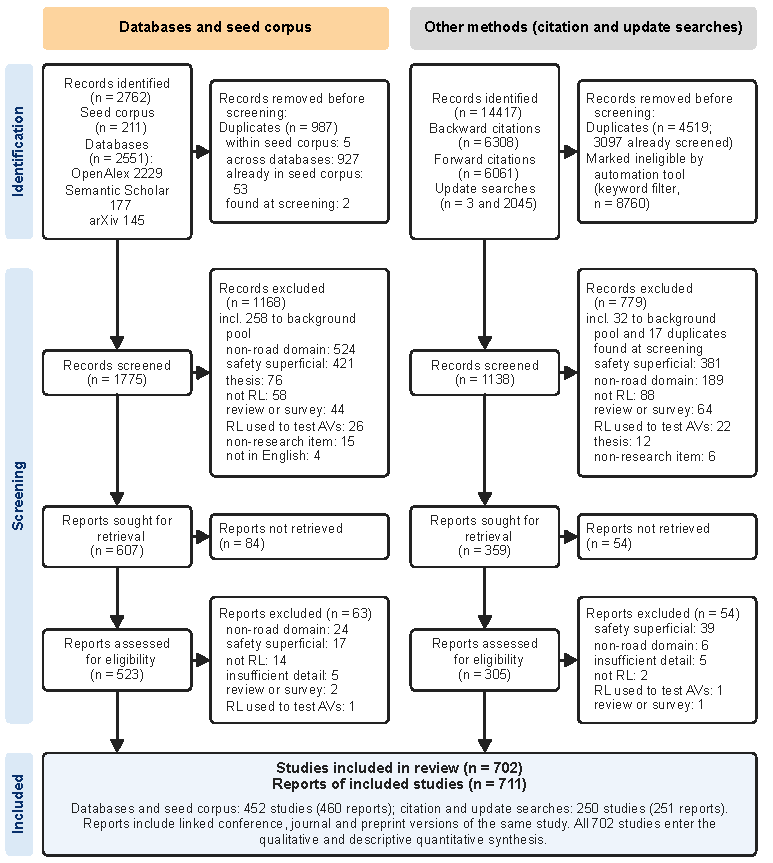
\includegraphics[width=\textwidth]{fig01_prisma}
\caption{PRISMA 2020 flow diagram of study identification, screening and inclusion through databases and the seed corpus (left) and through citation searching and two update searches (right). Counts are generated from the screening and full-text decision logs. EC codes refer to the exclusion criteria in Table~\ref{tab:criteria}; records outside road vehicles that develop Safe RL methods were placed in a background pool and are not counted as included studies. All \nIncluded{} included studies enter the synthesis; the reference list cites only those discussed in the text, and every included study is listed in Supplementary S3.}\label{fig:prisma}
\end{figure}

This section reports the outcome of the study selection and describes the evidence base, including when and where the studies were published, their quality, and how the field has evolved.

\subsection{Study selection}
The search identified \nRecIdent{} records: \nRecSeed{} from the seed corpus and \nRecDB{} from the databases (OpenAlex \nRecDBOpenAlex, Semantic Scholar \nRecDBSemanticScholar, arXiv \nRecDBarXiv). After \nDup{} duplicates were removed, \nScreened{} records were screened on title and abstract and \nScrExcluded{} were excluded (Fig.~\ref{fig:prisma}). The most common reasons were a non-road domain and safety that played no real role in the study; \nBackgroundPool{} of the non-road records were Safe RL method papers and were kept in a background pool for the conceptual discussion. Of the \nSought{} reports sought for retrieval, \nNotRetrieved{} could not be obtained and \nAssessed{} were assessed in full text. After \nFtExcluded{} exclusions, \nDbIncluded{} studies were included from the database search and seed corpus.

Citation searching and the two update searches identified \nCitRecords{} further records. After the removal of duplicates and records rejected by the keyword filter, \nCitScreened{} records were screened, and \nCitSought{} reports were sought; \nCitNotRetrieved{} could not be obtained, \nCitAssessed{} were assessed in full text, and \nCitIncluded{} studies were added. In total, \nIncluded{} studies were included, reported in \nReports{} reports (\nAddReports{} studies had a linked conference or preprint version). All included studies entered both the qualitative synthesis and the descriptive quantitative synthesis. The \nScrReviewsAll{} review and survey articles found during screening (\nScrReviews{} in the database search and \nCitReviews{} in citation searching) were not included as primary studies but were used to position this review (Table~\ref{tab:priorreviews}).

\subsection{Profile of the evidence base}
The field is young and growing quickly: \nYrRecentN{} studies (\nYrRecentP\%) appeared in 2025--2026 and a further \nYrMidN{} (\nYrMidP\%) in 2023--2024, whereas only \nYrEarlyN{} (\nYrEarlyP\%) predate 2021 (Fig.~\ref{fig:evolution}a). Journals accounted for \nPubJournalN{} studies (\nPubJournalP\%), conference proceedings for \nPubConferenceN{} (\nPubConferenceP\%), and preprints for \nPubPreprintN{} (\nPubPreprintP\%). Research groups in China (\nCtryChinaN; \nCtryChinaP\%) and the USA (\nCtryUSAN; \nCtryUSAP\%) dominated, followed by Germany (\nCtryGermanyN) and Singapore (\nCtrySingaporeN), with \nCtryCount{} countries represented in total. The most frequent outlets were IEEE Transactions on Intelligent Transportation Systems (\nVenTITS{} studies), arXiv (\nVenArxiv), the ITSC conference (\nVenITSC), the Intelligent Vehicles Symposium (\nVenIV), IEEE Transactions on Vehicular Technology (\nVenTVT), and IEEE Transactions on Intelligent Vehicles (\nVenTIV). Apart from arXiv, all of them are intelligent transportation and intelligent vehicle venues, indicating that the topic is driven mainly by the vehicle and transport communities.

\paragraph{Study quality.} The mean quality score was \nQAMean{} out of 24 (median \nQAMedian). In total, \nQAHighN{} studies (\nQAHighP\%) were of high quality, \nQAMediumN{} (\nQAMediumP\%) were of medium quality, and \nQALowN{} (\nQALowP\%) were of low quality (Table~\ref{tab:quality}). The item scores show a clear pattern. Studies usually state their objective (Q1, mean \nQAQOneMean), their Safe RL formulation (Q2, \nQAQTwoMean), and their experimental conditions (Q4, \nQAQFourMean) well. They are weakest on code and data availability (Q11, \nQAQOneOneMean), on testing under uncertainty or disturbance (Q8, \nQAQEightMean), on generalization (Q9, \nQAQNineMean), and on reproducibility (Q10, \nQAQOneZeroMean). The methods are generally described well, but the way they are tested is often weak. Journal articles score higher on average (\nQAJournal) than conference papers (\nQAConference) and preprints (\nQAPreprint).

%% BEGIN GENERATED tab12_quality
\begin{table}[!htbp]
\caption{Quality assessment of the included studies (each criterion scored 0, 1 or 2)}\label{tab:quality}
\footnotesize
\setlength{\tabcolsep}{3pt}
\begin{tabularx}{\textwidth}{@{}P{0.6cm} L P{0.9cm} P{1.1cm} P{1.1cm} P{1.1cm}@{}}
\toprule
Item & Criterion & Mean & Score 2 (\%) & Score 1 (\%) & Score 0 (\%) \\
\midrule
Q1 & Research objective clearly defined & 1.98 & 98.4 & 1.6 & 0.0 \\
Q2 & Safe RL formulation clearly described & 1.87 & 87.0 & 12.8 & 0.1 \\
Q3 & Safety mechanism explicitly defined & 1.69 & 69.7 & 29.9 & 0.4 \\
Q4 & Experimental conditions sufficiently described & 1.85 & 85.2 & 14.7 & 0.1 \\
Q5 & Meaningful baselines included & 1.46 & 50.1 & 45.6 & 4.3 \\
Q6 & Safety metrics reported & 1.68 & 70.8 & 26.4 & 2.8 \\
Q7 & Performance metrics reported & 1.85 & 85.6 & 14.1 & 0.3 \\
Q8 & Uncertainty or disturbance conditions evaluated & 1.05 & 30.3 & 44.7 & 24.9 \\
Q9 & Generalization evaluated & 1.00 & 31.9 & 36.6 & 31.5 \\
Q10 & Evaluation reproducible & 1.11 & 20.5 & 69.9 & 9.5 \\
Q11 & Code, data or simulator details available & 0.84 & 11.8 & 60.5 & 27.6 \\
Q12 & Evaluated beyond a trivial simulation & 1.31 & 38.3 & 54.4 & 7.3 \\
\midrule
\multicolumn{6}{@{}>{\raggedright\arraybackslash}p{\dimexpr\textwidth-1em\relax}@{}}{Total score (0--24): mean 17.7, median 18; bands: high ($\ge$18) 426 (60.7), medium (12--17) 236 (33.6), low ($\le$11) 40 (5.7).} \\
\multicolumn{6}{@{}>{\raggedright\arraybackslash}p{\dimexpr\textwidth-1em\relax}@{}}{Mean total by publication type: journal 18.7 ($n$=362); conference 16.5 ($n$=277); preprint 17.8 ($n$=63).} \\
\botrule
\end{tabularx}
\footnotetext{Scores and the justification of every score below 2 are in the extraction database (Supplementary S4).}
\end{table}
%% END GENERATED tab12_quality

\paragraph{Robustness of the findings.} The structural findings reported below do not depend on weaker studies. Across the four sensitivity subsets, the share of simulation-only studies stays between \nSensSimMin\% and \nSensSimMax\%, the share of studies reaching run-time enforcement (L3 or higher) between \nSensLThreeMin\% and \nSensLThreeMax\%, and code release between \nSensCodeMin\% and \nSensCodeMax\%. Indicators of evaluation practice are better in the high-quality subset (for example, studies without any generalization test fall from \nGenNoneP\% to \nSensHighNoGenP\%), but this is partly circular, because the quality items score those practices. A stricter high-quality band (total of 20 or more; \nQAStrictHighN{} studies) gives the same picture: \nQAStrictSimP\% of these studies are simulation-only and \nQAStrictLThreeP\% reach L3 or higher, against \nSimOnlyP\% and \nLThreePlusP\% in the full corpus.

Within the database search, the three retrieval rounds (open-access studies, paywalled IEEE studies, and paywalled studies from other publishers) had similar physical validation (\nGrpOAPhysP\%, \nGrpIEEEPhysP\%, and \nGrpRTwoPhysP\%) and comparable assurance levels (L3 or higher in \nGrpOALThreeP\%, \nGrpIEEELThreeP\%, and \nGrpRTwoLThreeP\%), but very different code release (\nGrpOACodeP\%, \nGrpIEEECodeP\%, and \nGrpRTwoCodeP\%). Retrieving the paywalled literature therefore changed the reproducibility picture more than the safety picture.

\paragraph{Effect of search scope.} The scope of the search matters more than access. Of the \nScopeCitN{} studies added by citation searching, \nScopeCitSafeTitleN{} used Safe RL terminology in their title, against \nScopeDbSafeTitleN{} of the \nScopeDbN{} database-search studies. This contrast is partly built in, because citation searching screened only records that the database queries, which contain these terms, had not already found; the comparison therefore describes the literature that the vocabulary misses rather than a random sample of RL-for-driving studies. Compared with the database-search studies, the citation-search studies reach run-time enforcement less often (\nScopeCitLThreeP\% vs \nScopeDbLThreeP\%), use constrained RL less often (\nScopeCitCmdpP\% vs \nScopeDbCmdpP\%) and rest on empirical evidence alone more often (L0--L1: \nScopeCitLOneP\% vs \nScopeDbLOneP\%), at a similar quality level. A search built on Safe RL vocabulary therefore over-represents the stronger mechanisms: the wider RL-for-driving literature, which treats safety mainly through the reward, is larger than such a search suggests. The proportions in this review describe the combined corpus and should be read with this scope effect in mind.

\subsection{How the field has evolved}
The field is often described as passing through four phases: basic RL first, then reward shaping and constrained RL, then barrier functions and robust methods, and finally foundation models, offline learning and runtime assurance. The data support this account only in part (Fig.~\ref{fig:evolution}b). Early work (2016--2020, \nPerOneN{} studies) was not ``basic RL'': shielding, filtering, or runtime assurance already appeared in \nPerOneShieldP\% of these studies and formal methods in \nPerOneFormalP\%, mostly to verify discrete driving decisions \citep{B0062}. Constrained RL then grew from \nPerOneConsP\% of studies to \nPerTwoConsP\% in 2021--2022, and barrier and Lyapunov methods grew steadily to \nPerFourCBFP\% in 2025--2026, while robust, risk-sensitive, and uncertainty-aware methods reached \nPerFourRobustP\%. Foundation-model-assisted RL appeared only in 2025--2026 (\nPerFourFMN{} studies). Formal methods, in contrast, fell to \nPerFourFormalP\% of recent studies.

The strength of the evidence has changed far less. The shares of studies reaching run-time enforcement were \nPerOneLThreeP\%, \nPerTwoLThreeP\%, \nPerThreeLThreeP\%, and \nPerFourLThreeP\% in the four periods; the share with physical or hardware-in-the-loop validation was \nPerOnePhysP\%, \nPerTwoPhysP\%, \nPerThreePhysP\%, and \nPerFourPhysP\%, and the share releasing code was \nPerOneCodeP\%, \nPerTwoCodeP\%, \nPerThreeCodeP\%, and \nPerFourCodeP\%. Trend tests across the four periods (Cochran--Armitage) find no change in run-time enforcement ($p=\nTrendLThreeP$) or code release ($p=\nTrendCodeP$), a rise in physical validation from a low base ($p=\nTrendPhysP$), and a fall in the share of formal methods ($p\nTrendFormalP$); 2026 is a partial year. Mean quality rose only modestly, from \nPerOneQA{} to \nPerFourQA. The field has broadened its methods faster than it has strengthened its evidence.

\begin{figure}[!htbp]
\centering
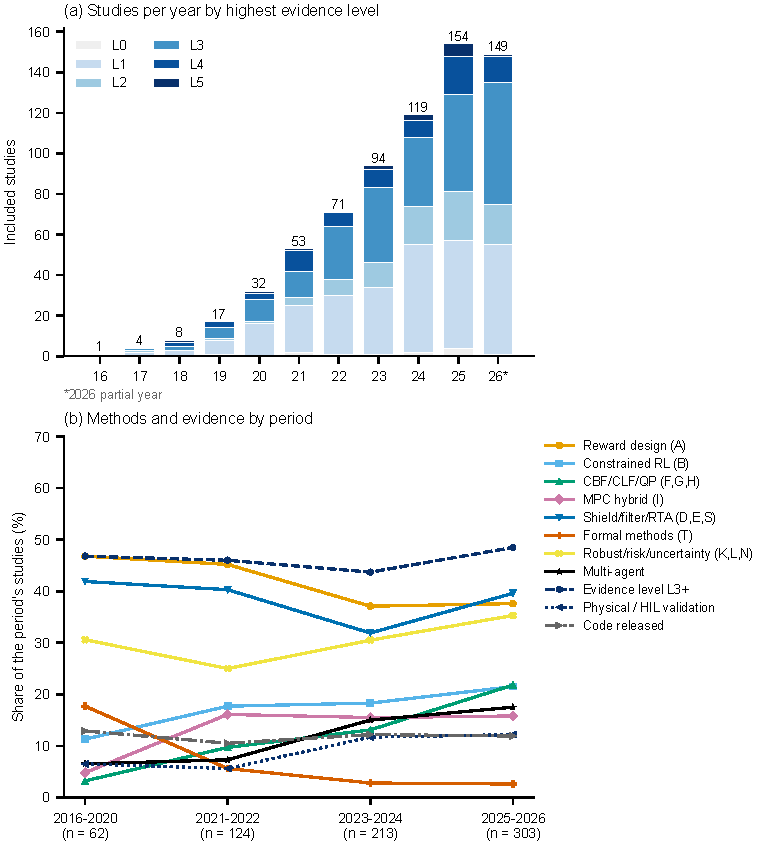
\includegraphics[width=\textwidth]{fig05_evolution}
\caption{Evolution of the field. (a) Included studies per publication year, shaded by the highest safety-evidence level each substantiates (review-derived levels L0--L5, Table~\ref{tab:levels}). (b) Share of each period's studies that use selected mechanism groups, reach run-time enforcement (L3+), include physical or hardware-in-the-loop validation, or release code. Methods broadened over time while the evidence indicators changed little.}\label{fig:evolution}
\end{figure}


%% =====================================================================
\section{Safety formulations, RL methods and a taxonomy of safety mechanisms}\label{sec:taxonomy}
%% =====================================================================

This section answers RQ1--RQ3 and RQ5: how safety is defined and represented, which RL methods are used, and which mechanisms provide safety. It ends with a critical appraisal of each family of mechanisms.

\subsection{How safety is formulated (RQ1, RQ2)}
The included studies rarely define safety formally. Instead, they \emph{operationalize} it through what they measure or enforce. Only \nSafetyCostN{} studies (\nSafetyCostP\%) define an explicit safety cost signal separate from the reward, for example, a collision indicator, a time-to-collision (TTC) threshold, a distance violation, or a risk field. The remainder encode safety through the reward, through constraints in an optimization layer, or through rules and safe sets that act on the actions. Table~\ref{tab:notions} shows the type of safety claim made by the studies. Most (\nClaimEmpN; \nClaimEmpP\%) make an empirical claim, \nClaimRtN{} (\nClaimRtP\%) a run-time enforcement claim, \nClaimCexpN{} (\nClaimCexpP\%) a claim of constraint satisfaction in expectation, and \nClaimFormalN{} (\nClaimFormalP\%) a formal claim. Probabilistic (\nClaimProbN), robust (\nClaimRobN), and statistically tested (\nClaimStatN) claims are uncommon. Importantly, \nClaimEmpOnlyN{} studies (\nClaimEmpOnlyP\%) make \emph{only} an empirical claim.

The safety acts also vary. In \nStageTrainN{} studies (\nStageTrainP\%), every safety mechanism acts only during training, for example, a penalty or constraint that shapes the learned policy but is absent when the policy runs. In \nStageBothN{} (\nStageBothP\%) safety acts during both training and execution, and in \nStageExecN{} (\nStageExecP\%) only during execution, typically through a filter wrapped around an already trained policy. This distinction matters because only mechanisms that act at execution can protect the vehicle against the policy's own errors after deployment.

%% BEGIN GENERATED tab01_notions
\begin{sidewaystable}
\caption{Notions of safety used in Safe RL for autonomous vehicles, what each establishes, and how often included studies make each kind of claim (a study can make several)}\label{tab:notions}
\scriptsize
\setlength{\tabcolsep}{3pt}
\begin{tabularx}{\textheight}{@{}P{2.0cm} L P{3.6cm} P{2.4cm} P{1.8cm} P{3.4cm}@{}}
\toprule
Notion & What is established & Typical formulation & Foundations & Studies, $n$ (\%) & Example \\
\midrule
Empirical & Unsafe events were rare in the tested episodes and scenarios & Collision, success or violation rates in simulation or tests &  & 589 (83.9); only claim: 315 (44.9) & \citealp{C0438} \\
Statistical & As empirical, with confidence intervals or hypothesis tests over episodes & Repeated seeds, bootstrap intervals, significance tests &  & 22 (3.1) & \citealp{B0754} \\
Constraint satisfaction in expectation & Expected cumulative cost stays below a budget & Constrained MDP solved by Lagrangian, trust-region or projection methods & \citep{altman1999cmdp,achiam2017cpo} & 108 (15.4) & \citealp{B0896} \\
Probabilistic & Safety holds with a stated probability under a stochastic model & Chance constraints, Gaussian-process or conformal bounds, CVaR &  & 20 (2.8) & \citealp{B0972} \\
Robust & Safety holds for every perturbation in a bounded set & Adversarial training, robust MPC/CBF, bounded-disturbance tubes &  & 58 (8.3) & \citealp{A089} \\
Run-time enforced & Each executed action is checked or corrected online, given the monitor's model & Shields, safety filters, runtime assurance (Simplex-type fallback) & \citep{alshiekh2018shielding} & 198 (28.2) & \citealp{B0678} \\
Formal & A property (invariance, reachability, temporal-logic specification) is proved or verified under explicit assumptions & CBF/CLF certificates, Hamilton--Jacobi or set reachability, model checking & \citep{ames2017cbfqp,ames2019cbf} & 92 (13.1) & \citealp{A089} \\
Toward certification & Run-time or formal safety carried onto a physical vehicle with a safety analysis; ultimately a safety case against automotive standards & Physical tests with violation statistics; assurance arguments (e.g.\ ISO 26262, ISO 21448) &  & L5: 15 (2.1); safety case: 1 & \citealp{B0678}; safety case \citealp{B1443} \\
\botrule
\end{tabularx}
\footnotetext{Percentages of the 702 included studies. Claim types are coded per study (Supplementary S3). Example: a study matching the row, chosen by primary mechanism (where applicable), journal article in a JCR Q1/Q2 journal, highest safety-evidence level, quality score and recency; all studies are listed in the extraction database (Supplementary S3).}
\end{sidewaystable}
%% END GENERATED tab01_notions

\subsection{Reinforcement-learning methods (RQ3)}
Model-free learning dominates (\nParMFN{} studies; \nParMFP\%). The most common algorithm families are off-policy actor-critic methods (\nFamOffPolN; \nFamOffPolP\%), value-based methods (\nFamValueN; \nFamValueP\%), on-policy policy-gradient methods (\nFamOnPolN; \nFamOnPolP\%), and dedicated constrained policy-optimization methods (\nFamConPolN; \nFamConPolP\%) (Table~\ref{tab:algorithms}). The most frequent individual algorithms are PPO (\nAlgPPON), SAC (\nAlgSACN), DQN (\nAlgDQNN), DDPG (\nAlgDDPGN), and TD3 (\nAlgTDThreeN), followed by Double DQN (\nAlgDDQNN), the Lagrangian variants of SAC (\nAlgSACLagN) and PPO (\nAlgPPOLagN), and CPO (\nAlgCPON). Hierarchical RL appears in \nParHRLN{} studies (\nParHRLP\%), model-based learning in \nParMBN{} (\nParMBP\%), imitation combined with RL in \nParILRLN{} (\nParILRLP\%), offline or offline-to-online learning in \nParOfflineN{} (\nParOfflineP\%), and assistance from large language or vision-language models in \nParLLMN{}. A Lagrangian or primal--dual solution is used in \nLagN{} studies (\nLagP\%), and any constrained formulation in \nAnyConstrN{} (\nAnyConstrP\%).

The choice of algorithm says little about safety. Every algorithm family is paired with every kind of safety mechanism (Fig.~\ref{fig:algmech}); the safety property comes from the mechanism wrapped around the algorithm, not from the algorithm itself. Within constrained RL, four observations recur. First, plain Lagrangian methods are sensitive to the multiplier and its initialization \citep{B1312}, and some studies switch to PID-controlled multipliers for this reason \citep{B1490}. Second, they oscillate around the constraint during training, which recent work has damped with proportional--integral or augmented-Lagrangian terms \citep{B1312}. Third, because the constraint holds only on average, dangerous long-tail behavior can remain \citep{B0658}, which motivates worst-case and CVaR variants \citep{B1798} and per-component cost critics \citep{B1712}. Finally, several ``constrained'' methods constrain robustness, similarity to human driving, driver fear, or user preference rather than physical safety \citep{B1566}; therefore, the presence of a constraint alone does not guarantee safety.

Policies are mostly small multilayer perceptrons (\nNetMLPN; \nNetMLPP\%) that act on state vectors (\nObsVECN; \nObsVECP\%). Camera images were used in \nObsIMGN{} studies (\nObsIMGP\%), bird's-eye-view rasters in \nObsBEVN{} (\nObsBEVP\%), and LiDAR in \nObsLIDARN{} (\nObsLIDARP\%). Safe RL therefore operates mainly on states that a separate perception system has already produced; we return to this point in the safety-stack analysis (Sect.~\ref{sec:discussion}). Policies output low-level control in \nActCtrlN{} studies (\nActCtrlP\%), behavior-level decisions such as lane choices in \nActBehavN{} (\nActBehavP\%), trajectories in \nActTrajN{} (\nActTrajP\%), and controller parameters in \nActParamN{} (\nActParamP\%).

%% BEGIN GENERATED tab02_algorithms
\begin{table}[!htbp]
\caption{RL algorithm families, their most frequent algorithms, the safety mechanisms they are paired with, and the resulting strength of safety evidence}\label{tab:algorithms}
\scriptsize
\setlength{\tabcolsep}{3pt}
\begin{tabularx}{\textwidth}{@{}P{2.2cm} P{1.2cm} L P{0.9cm} P{1.6cm} P{0.7cm} P{2.2cm}@{}}
\toprule
Family & $n$ (\%) & Most frequent algorithms ($n$) & Constr.\ (\%) & Main clusters ($n$) & L3+ (\%) & Example \\
\midrule
Off-policy actor-critic & 247 (35.2) & SAC (105); DDPG (72); TD3 (59) & 7.7 & M1 (161); M2 (123) & 46.6 & \citealp{B0678} \\
Value-based & 185 (26.4) & DQN (88); Double DQN (42); Dueling double DQN (17) & 4.9 & M1 (107); M2 (98) & 50.8 & \citealp{C0194} \\
On-policy policy gradient & 152 (21.7) & PPO (123); MAPPO (14); A2C (8) & 7.9 & M1 (89); M6 (73) & 44.7 & \citealp{A140} \\
Constrained policy optimization & 87 (12.4) & SAC-Lagrangian (23); PPO-Lagrangian (16); CPO (12) & 100.0 & M1 (86); M6 (35) & 21.8 & \citealp{B0896} \\
Model-based RL & 31 (4.4) & Adaptive dynamic programming (12); Model-based AC (8); Model-based RL + MPC (3) & 38.7 & M6 (20); M3 (18) & 58.1 & \citealp{B0972} \\
Offline RL & 14 (2.0) & CQL (4); Constrained decision transformer (2); BCQ (1) & 21.4 & M6 (14); M1 (7) & 28.6 & \citealp{C0998} \\
Generic actor-critic & 17 (2.4) & Actor-critic (14); Adversarial robust AC (3) & 23.5 & M3 (10); M5 (9) & 58.8 & \citealp{B1409} \\
Other / unspecified & 19 (2.7) & Not reported (6); MCTS (5); Various (2) & 5.3 & M2 (10); M6 (10) & 63.2 & \citealp{B1333} \\
\midrule
\multicolumn{7}{@{}>{\raggedright\arraybackslash}p{\dimexpr\textwidth-1em\relax}@{}}{Paradigms (a study can use several): model-free 637 (90.7); hierarchical 85 (12.1); model-based 65 (9.3); imitation + RL 61 (8.7); offline or offline-to-online 21 (3.0); LLM-assisted 11 (1.6).} \\
\multicolumn{7}{@{}>{\raggedright\arraybackslash}p{\dimexpr\textwidth-1em\relax}@{}}{Constrained formulations: Lagrangian or primal--dual solution 72 (10.3); any constrained formulation 136 (19.4).} \\
\botrule
\end{tabularx}
\footnotetext{Constr.: studies of the family using a Lagrangian/primal--dual solution or a constrained (CMDP) formulation. Clusters M1--M6 as in Fig.~\ref{fig:taxonomy}. L3+/L4+: share of the row's studies whose highest substantiated evidence level is at least L3/L4. Example: a study matching the row, chosen by primary mechanism (where applicable), journal article in a JCR Q1/Q2 journal, highest safety-evidence level, quality score and recency; all studies are listed in the extraction database (Supplementary S3).}
\end{table}
%% END GENERATED tab02_algorithms

\begin{figure}[!htbp]
\centering
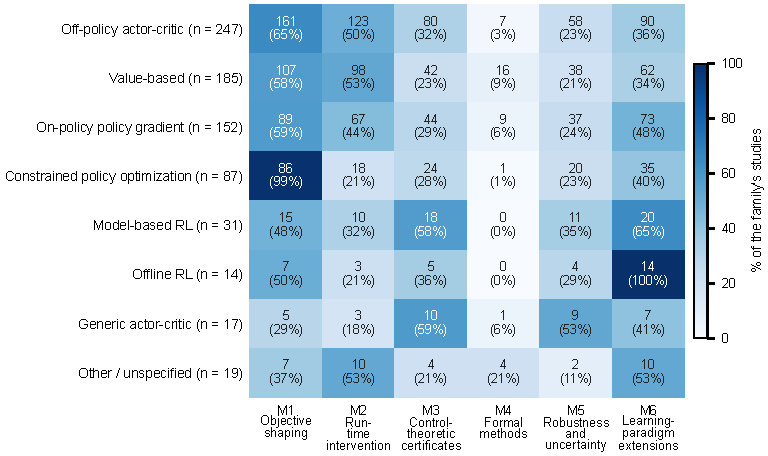
\includegraphics[width=\textwidth]{fig07_algorithm_mechanism}
\caption{RL algorithm family versus safety-mechanism cluster (number of studies and share of the family's studies). Constrained policy optimization belongs to cluster M1 by construction. Every family is paired with every kind of mechanism, so the algorithm says little about how safety is obtained.}\label{fig:algmech}
\end{figure}

\subsection{A two-layer taxonomy of safety mechanisms (RQ5)}
The codebook defined 24 mechanism categories: the 22 proposed in the protocol, plus rule-based intervention and foundation-model assistance, which were added when the codebook was built. All were observed except one: no included study uses distributionally robust RL. Most studies combine mechanisms: only \nMechSingleN{} (\nMechSingleP\%) use a single mechanism, while \nMechMultiN{} (\nMechMultiP\%) combine two or more. A taxonomy built on single labels would therefore misrepresent the field. We use two layers instead (Fig.~\ref{fig:taxonomy}). The first layer groups mechanisms into six review-derived clusters according to \emph{where} safety enters the learning-and-control loop:
\begin{itemize}
\item \textbf{M1 Objective shaping} (\nClMOneN{} studies; \nClMOneP\%): safety acts inside the learning objective, through reward design, constrained RL, safety critics or risk-sensitive objectives.
\item \textbf{M2 Run-time intervention} (\nClMTwoN; \nClMTwoP\%): safety acts between the policy and the actuators, through shields and action masks, safety filters, runtime assurance or rule-based intervention.
\item \textbf{M3 Control-theoretic certificates} (\nClMThreeN; \nClMThreeP\%): safety comes from a certificate or an optimization layer, namely CBFs, CLFs, CBF-CLF quadratic programs, MPC or reachable sets.
\item \textbf{M4 Formal methods} (\nClMFourN; \nClMFourP\%): safety comes from a verified model or specification.
\item \textbf{M5 Robustness and uncertainty} (\nClMFiveN; \nClMFiveP\%): safety comes from an explicit model of perturbations or uncertainty.
\item \textbf{M6 Learning-paradigm extensions} (\nClMSixN; \nClMSixP\%): the way data and agents are organized, through multi-agent, offline, model-based, hierarchical, sim-to-real, human-in-the-loop or foundation-model-assisted learning.
\end{itemize}
The second layer is the individual mechanism (Table~\ref{tab:mechanisms}). Five studies contribute no safety mechanism of their own: two benchmarks \citep{B0272,C0328}, a safety-oriented state representation \citep{B1178}, a safety case for an RL component \citep{B1443} and an RL-tuned risk-assessment monitor that flags critical situations without acting on the vehicle \citep{C0550}.

\begin{figure}[!htbp]
\centering
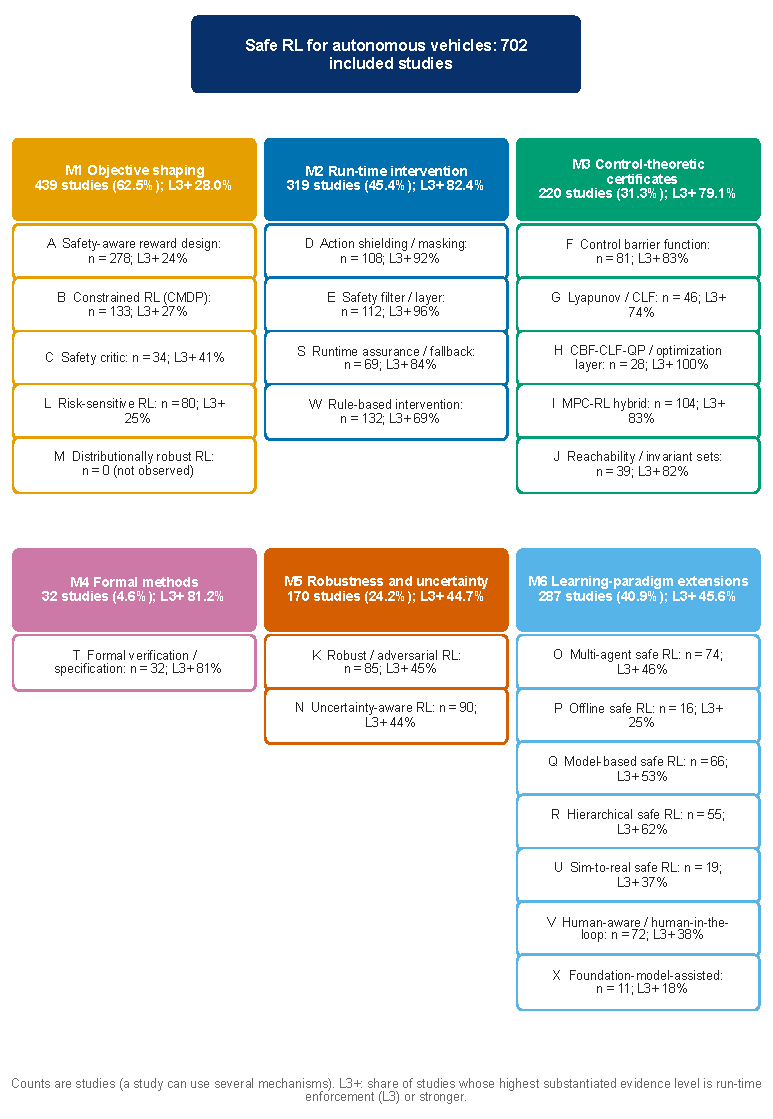
\includegraphics[width=\textwidth,height=0.86\textheight,keepaspectratio]{fig02_taxonomy}
\caption{Evidence-driven two-layer taxonomy of Safe RL for autonomous vehicles. Clusters M1--M6 group the coded safety mechanisms by where safety enters the learning-and-control loop. Counts are studies (a study can use several mechanisms); L3+ is the share of studies reaching run-time enforcement or stronger evidence.}\label{fig:taxonomy}
\end{figure}

The clusters differ sharply in the strength of the evidence they produce (Fig.~\ref{fig:mechevidence}). Part of this split follows from the definition of the levels: L3 requires a mechanism that acts at runtime; therefore, a study without a runtime or certificate mechanism cannot reach it, and none does. The informative part is the converse. Of the \nRtMechN{} studies that use a runtime or certificate mechanism, \nRtMechBelowN{} (\nRtMechBelowP\%) stay below L3: \nRtMechBelowTrainN{} because the barrier, mask, or controller acts only during training, for example, as a loss term or a training-time mask, and the others because the enforcement is not evaluated or does not act on every executed action. Having a safety layer and using it at runtime are therefore not the same, and the mechanism label alone overstates the evidence. Objective-shaping mechanisms rarely reach runtime or formal levels on their own. Only \nMechALThreeP\% of the studies using reward design reach L3 or higher, always through another mechanism, and \nMechAEmpOnlyP\% make only an empirical claim. Constrained-RL studies reach L3 or higher in \nMechBLThreeP\% of cases; their typical claim is constraint satisfaction in expectation, which is stronger than an empirical claim but still not a per-step guarantee. By contrast, studies using safety filters reach L3 or higher in \nMechELThreeP\% of cases; shields and masks in \nMechDLThreeP\%, CBF-CLF quadratic programs in \nMechHLThreeP\%, MPC hybrids in \nMechILThreeP\%, CBFs in \nMechFLThreeP\% and reachability in \nMechJLThreeP\%. Formal properties (L4 or higher) are most common for reachability (\nMechJLFourP\%), CBF-CLF quadratic programs (\nMechHLFourP\%), formal methods (\nMechTLFourP\%) and CBFs (\nMechFLFourP\%). Learning-paradigm extensions inherit the level of the mechanism they are paired with. Only four of the \nMechPN{} offline studies reach L3 or higher, each through a runtime layer added to the offline policy: a gradient-based action correction with a learned reachability value \citep{B1162}, a constrained trajectory optimizer \citep{C0748}, execution-authority gating with a rule-based fallback \citep{C0998}, and a CBF-MPC filter that also protects online fine-tuning and was carried onto a small unmanned ground vehicle \citep{E060}. The \nMechXN{} foundation-model-assisted studies reach L3 only twice, both through a barrier layer: an MPC-CBF layer \citep{B1584} and a CBF quadratic program on the executed command \citep{E035}.

%% BEGIN GENERATED tab03_mechanisms
\begin{sidewaystable}
\caption{Safety mechanisms by review-derived cluster: frequency, when they act, the strength of safety evidence they reach, and physical validation}\label{tab:mechanisms}
\scriptsize
\setlength{\tabcolsep}{3pt}
\begin{tabularx}{\textheight}{@{}P{0.3cm} P{3.8cm} P{1.4cm} P{1.0cm} P{0.9cm} P{0.9cm} P{1.0cm} L@{}}
\toprule
 & Mechanism & $n$ (\%) & Exec.\ (\%) & L3+ (\%) & L4+ (\%) & Emp.\ only (\%) & Physical/HIL $n$; examples \\
\midrule
\multicolumn{8}{@{}>{\raggedright\arraybackslash}p{\dimexpr\textheight-1em\relax}@{}}{\textit{M1 Objective shaping}} \\
A & Safety-aware reward design & 278 (39.6) & 33.8 & 24.1 & 1.4 & 80.2 & 14; \citealp{C0281} \\
B & Constrained RL (CMDP) & 133 (18.9) & 28.6 & 27.1 & 6.8 & 8.3 & 20; \citealp{B0896} \\
C & Safety critic & 34 (4.8) & 44.1 & 41.2 & 5.9 & 29.4 & 4; \citealp{C1049} \\
L & Risk-sensitive RL & 80 (11.4) & 37.5 & 25.0 & 3.8 & 51.2 & 6; \citealp{B1175} \\
M & Distributionally robust RL & 0 & -- & -- & -- & -- & not observed \\
\multicolumn{8}{@{}>{\raggedright\arraybackslash}p{\dimexpr\textheight-1em\relax}@{}}{\textit{M2 Run-time intervention}} \\
D & Action shielding / masking & 108 (15.4) & 94.4 & 91.7 & 20.4 & 36.1 & 9; \citealp{B0754} \\
E & Safety filter / layer & 112 (16.0) & 99.1 & 96.4 & 27.7 & 8.0 & 13; \citealp{B1536} \\
S & Runtime assurance / fallback & 69 (9.8) & 85.5 & 84.1 & 23.2 & 31.9 & 18; \citealp{B0678} \\
W & Rule-based intervention & 132 (18.8) & 82.6 & 68.9 & 6.1 & 56.1 & 12; \citealp{B1778} \\
\multicolumn{8}{@{}>{\raggedright\arraybackslash}p{\dimexpr\textheight-1em\relax}@{}}{\textit{M3 Control-theoretic certificates}} \\
F & Control barrier function & 81 (11.5) & 84.0 & 82.7 & 44.4 & 4.9 & 9; \citealp{B0327} \\
G & Lyapunov / CLF & 46 (6.6) & 78.3 & 73.9 & 50.0 & 13.0 & 4; \citealp{B1508} \\
H & CBF-CLF-QP / optimization layer & 28 (4.0) & 100.0 & 100.0 & 53.6 & 0.0 & 3; \citealp{B1777} \\
I & MPC-RL hybrid & 104 (14.8) & 93.3 & 82.7 & 16.3 & 24.0 & 18; \citealp{B0485} \\
J & Reachability / invariant sets & 39 (5.6) & 84.6 & 82.1 & 64.1 & 10.3 & 7; \citealp{B0634} \\
\multicolumn{8}{@{}>{\raggedright\arraybackslash}p{\dimexpr\textheight-1em\relax}@{}}{\textit{M4 Formal methods}} \\
T & Formal verification / specification & 32 (4.6) & 81.2 & 81.2 & 56.2 & 12.5 & 1; \citealp{C0194} \\
\multicolumn{8}{@{}>{\raggedright\arraybackslash}p{\dimexpr\textheight-1em\relax}@{}}{\textit{M5 Robustness and uncertainty}} \\
K & Robust / adversarial RL & 85 (12.1) & 54.1 & 44.7 & 28.2 & 8.2 & 13; \citealp{B1409} \\
N & Uncertainty-aware RL & 90 (12.8) & 62.2 & 44.4 & 8.9 & 51.1 & 10; \citealp{B1093} \\
\multicolumn{8}{@{}>{\raggedright\arraybackslash}p{\dimexpr\textheight-1em\relax}@{}}{\textit{M6 Learning-paradigm extensions}} \\
O & Multi-agent safe RL & 74 (10.5) & 56.8 & 45.9 & 14.9 & 43.2 & 4; \citealp{C1051} \\
P & Offline safe RL & 16 (2.3) & 37.5 & 25.0 & 6.2 & 37.5 & 1; \citealp{B0930} \\
Q & Model-based safe RL & 66 (9.4) & 65.2 & 53.0 & 13.6 & 30.3 & 12; \citealp{B1793} \\
R & Hierarchical safe RL & 55 (7.8) & 70.9 & 61.8 & 5.5 & 52.7 & 3; \citealp{B1459} \\
U & Sim-to-real safe RL & 19 (2.7) & 47.4 & 36.8 & 31.6 & 31.6 & 12; \citealp{B1189} \\
V & Human-aware / human-in-the-loop & 72 (10.3) & 45.8 & 37.5 & 8.3 & 63.9 & 12; \citealp{B1167} \\
X & Foundation-model-assisted & 11 (1.6) & 27.3 & 18.2 & 0.0 & 72.7 & 0; \citealp{B1651} \\
\botrule
\end{tabularx}
\footnotetext{Exec.: mechanism acts at execution time (alone or in addition to training). Emp.\ only: the study's only safety claim is empirical. L3+/L4+: share of the row's studies whose highest substantiated evidence level is at least L3/L4. Example: a study matching the row, chosen by primary mechanism (where applicable), journal article in a JCR Q1/Q2 journal, highest safety-evidence level, quality score and recency; all studies are listed in the extraction database (Supplementary S3).}
\end{sidewaystable}
%% END GENERATED tab03_mechanisms

\begin{figure}[!htbp]
\centering
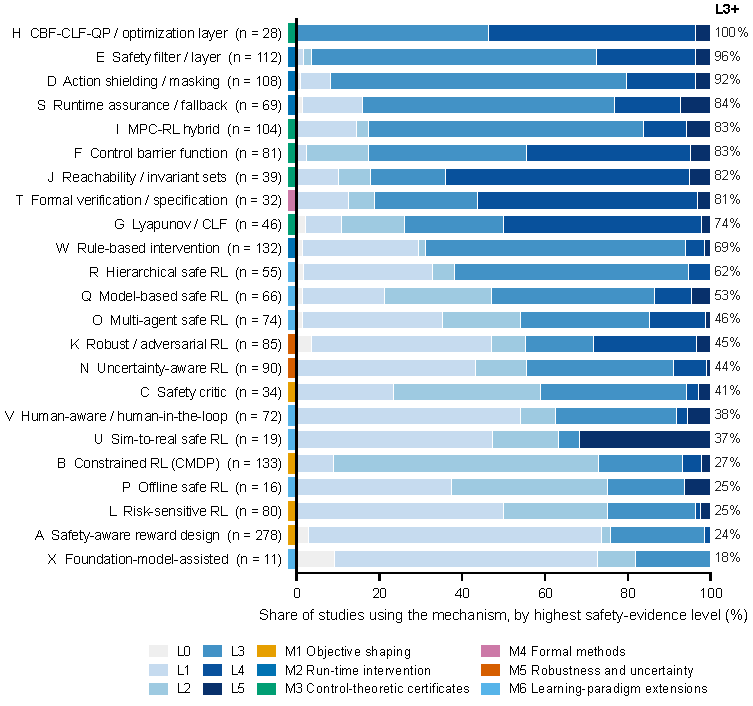
\includegraphics[width=\textwidth]{fig04_mechanism_evidence}
\caption{Safety-evidence profile of each mechanism: share of the studies using the mechanism at each highest evidence level (L0--L5), sorted by the share at L3 or above. The colored marker shows the mechanism's cluster. Objective-shaping mechanisms (reward design, constrained RL, risk-sensitive RL) rarely reach run-time or formal levels unless they are combined with a run-time or certificate mechanism.}\label{fig:mechevidence}
\end{figure}

\subsection{Critical appraisal of the mechanism families}\label{sec:appraisal}
Each family is appraised below against the same questions: what it does and why, how it provides safety and what that assumes, its advantages and limitations, the evidence behind it, and how well it is likely to transfer to real vehicles. Advantages are listed separately only when they go beyond motivation.

\subsubsection{Safety-aware reward design}

\emph{What and why.} Reward design adds penalties for collisions, risk fields, small time gaps, and similar quantities to the reward \citep{B1487}, sometimes encoding traffic rules as a reward machine \citep{B0432} or adding a predictive overlap forecast \citep{B0847}. It is popular because it is simple and requires no extra machinery (\nMechAN{} studies).

\emph{Safety and assumptions.} Safety is provided only indirectly by making unsafe behavior costly on average, and it assumes that the chosen weights encode the right trade-off.

\emph{Limitations.} The weights are brittle: a penalty-tuned PPO agent failed when the traffic dynamics changed, whereas a constrained agent did not \citep{B0221}; the shape of the penalty alone moved left-turn success between 28\% and 73\% in one study \citep{B1556}; and a predictive risk reward still needed an inference-time guard to push collisions below 1\% \citep{B0847}. Reward design provides no per-state or per-step assurance.

\emph{Evidence and transfer.} Only \nMechALThreeP\% of these studies reach L3 or higher, always through other mechanisms, and \nMechAEmpOnlyP\% make only an empirical claim. Reward design is a baseline rather than a safety method; it is best used to shape comfort and efficiency on top of a constraint or a filter.

\subsubsection{Constrained RL and safety critics}

\emph{What and why.} These methods formulate the task as a CMDP and solve it with Lagrangian, trust-region, or projection methods \citep{B0893}, often with learned cost critics that predict future constraint violations \citep{A099} (\nMechBN{} and \nMechCN{} studies). They separate safety from reward and replace weight tuning with a single, interpretable cost budget \citep{B0221}, which can even be adapted to a driver's risk preference \citep{B0976}.

\emph{Safety and assumptions.} The expected cumulative cost is maintained below the budget. This assumes that the cost signal captures the hazard and that the budget is meaningful.

\emph{Limitations.} The constraint holds only in expectation; therefore, rare catastrophic states remain possible, which has motivated uniformly state-wise constraints \citep{B0658} and state-wise Lagrangians \citep{B0445}. Violations occur while the agent learns \citep{B0575}, training is sensitive to the multiplier \citep{B1312}, and certificates added only as training losses do not act at runtime \citep{B1168}.

\emph{Evidence and transfer.} Of the constrained-RL studies, \nMechBLThreeP\% reached L3 or higher, and \nMechBPhys{} had physical or hardware-in-the-loop evidence, more than any other mechanism. The strongest results pair the constraint with a run-time layer, for example Lagrangian SAC with an MPC shield on a real off-road vehicle \citep{B0896}, constrained policy optimization with a rollover shield on a 1/10-scale car \citep{B0757}, or a bounded residual over MPC \citep{B1761}. Constrained RL transfers better than reward design but is weaker than run-time layers for per-step safety.

\subsubsection{Shielding, masking and rule-based intervention}

\emph{What and why.} These mechanisms remove or replace unsafe actions before execution (\nMechDN{} studies with shields or masks, \nMechWN{} with rule-based intervention). The decision is based on predictions \citep{B0028,B0886}, worst-case checks \citep{B1281}, occupancy or reachable sets \citep{B1450,B0778}, friction-aware risk assessment \citep{B0754}, logic rules \citep{C0194}, or formally verified models \citep{B0062}. Their appeal is that, from the first episode onwards, exploration never takes an action that the shield marks as unsafe.

\emph{Safety and assumptions.} A discrete check acts on every action. It assumes that the rule or model is complete and correct and that perception is accurate.

\emph{Limitations.} Shields can be conservative \citep{B1281,B0754} and lead to suboptimal policies \citep{B0028}; handwritten rules scale poorly \citep{B0381}; learned shields are only as reliable as their training data \citep{B1787}; some masks act only during training \citep{B1450}; and clipping masks for continuous actions carry no formal guarantee, as some authors state explicitly \citep{B0987}.

\emph{Evidence and transfer.} Shielding studies reached L3 or higher in \nMechDLThreeP\% of cases and L4 or higher in \nMechDLFourP\%; rule-based intervention reached L3 or higher in \nMechWLThreeP\%. Of the \nMechDPhys{} shielding studies with physical evidence, \nMechDLFive{} reached L5 \citep{B0028,B0444,B0896,B0757}. Shielding is the natural partner of decision-level RL and transfers well to the decision layer, provided that its perception assumptions hold.

\subsubsection{Safety filters and runtime assurance}

\emph{What and why.} A safety filter minimally modifies the RL action, for example by an action governor \citep{A072}, a projection onto a feasible domain \citep{B1169}, an MPC-based projection \citep{B1658} or a quadratic program \citep{B1445} (\nMechEN{} studies). Runtime assurance switches to a verified or conservative fallback when a monitor detects danger (\nMechSN{} studies): a Simplex architecture \citep{B0257}, an uncertainty-triggered switch to a rule-based driver model \citep{A096}, an MPC supervisor \citep{A140}, an ensemble-uncertainty switch to risk-adaptive MPC \citep{B0653} or a fallback to a rule-based policy whenever the RL action is not valued higher \citep{B1333}. Both keep RL's performance while bounding its failures at execution time.

\emph{Safety and assumptions.} Safety is enforced at every step. This assumes a correct safe set or backup controller and a monitor that detects danger in a timely way.

\emph{Limitations.} The policy may learn to rely on the filter \citep{B0886}, although feeding the correction back into training can reduce this \citep{B0987}; frequent interventions reduce performance \citep{B0301}; and fallbacks can be overly conservative \citep{A096,B1093}.

\emph{Evidence and transfer.} Filters reached L3 or higher in \nMechELThreeP\% of the studies. Runtime assurance had \nMechSPhys{} studies with physical or hardware-in-the-loop evidence, second only to constrained RL, including a closed-course test with MPC expert takeover \citep{A140}, public-road deployment \citep{B0761}, and processor-in-the-loop tests \citep{A096,B1093}. This is the most deployment-ready family because it matches how automotive safety architectures are already built: a monitor plus a fallback.

\subsubsection{Barrier and Lyapunov certificates}

\emph{What and why.} CBFs enforce the forward invariance of a safe set, and CLFs add stability (\nMechFN{}, \nMechGN{}, and \nMechHN{} studies used CBFs, CLFs or Lyapunov functions, and CBF-CLF quadratic programs, respectively). The certificate acts through a QP at runtime \citep{B0750} or through a constraint or loss term during the learning process \citep{A086,B1168}. A separate line of work designs barrier-Lyapunov backstepping controllers, whose gains or value functions are learned by adaptive dynamic programming \citep{B1508}. Certificates offer formal invariance properties at low computational costs.

\emph{Safety and assumptions.} Invariance holds at every step, given a control-affine model, a valid barrier, a feasible QP, and an accurate state.

\emph{Advantages.} Certificates provide the strongest guarantees per unit of computation; they extend to multi-agent and platoon-level safety \citep{B0327}, including the protection of following human drivers \citep{B0974}; and they can be combined with learning to reduce conservatism \citep{A204} or with Gaussian-process uncertainty and attack bounds to set robust margins \citep{B1777}.

\emph{Limitations.} Non-affine and discrete-time dynamics make the filter difficult to compute \citep{B1533}; single-step barriers ignore input limits \citep{B0968}; attacks on the state input \citep{A164} and friction changes \citep{A053} break the guarantee; barriers used only as soft regularizers lose it \citep{A086,B1168}; and the adaptive-dynamic-programming line proves boundedness only in numerical examples without traffic. These limitations match the open problems identified for Lyapunov- and barrier-based Safe RL in general: certificate validity under function approximation and distribution shift, feasibility and deadlock of hard CBF-QP shielding, and scaling to high-dimensional, partially observable settings \citep{kushwaha2026lyapunov}.

\emph{Evidence and transfer.} L4 or higher is reached by \nMechFLFourP\% of CBF studies, \nMechGLFourP\% of CLF or Lyapunov studies and \nMechHLFourP\% of CBF-CLF-QP studies; \nMechFPhys{} CBF studies have physical evidence, and one is the only filter of any kind supervising an RL policy on a production vehicle in public traffic \citep{B0761}. Certificates are stronger than CMDPs for per-step safety and cheaper than MPC; their transfer depends on whether the model and perception assumptions can be bounded.

\subsubsection{MPC--RL hybrids}

\emph{What and why.} MPC is placed alongside RL as a low-level planner under RL decisions \citep{B1780}, as a controller tuned by RL or given a learned terminal cost \citep{A204,B1041}, as a safety layer \citep{A089,B1536}, as an expert and fallback \citep{A140} or as the backbone under a bounded RL residual \citep{B1169,B1761} (\nMechIN{} studies). MPC handles constraints explicitly while RL handles interaction and long-horizon intent.

\emph{Safety and assumptions.} Constraints are satisfied over the prediction horizon, which assumes accurate predictions of other agents and recursive feasibility, the latter of which is often cited rather than proven \citep{B1658}.

\emph{Limitations.} MPC is computationally expensive \citep{B0446}, although learning the solver can reduce the cost by two orders of magnitude \citep{B1137}; it depends on prediction models, often constant-velocity ones \citep{B0053}; and the guarantee is lost when the MPC is infeasible \citep{A204,B0972}.

\emph{Evidence and transfer.} Of the MPC hybrids, \nMechILThreeP\% reach L3 or higher, and \nMechILFourP\% reach L4 or higher; \nMechIPhys{} have physical or hardware-in-the-loop evidence on real vehicles \citep{B0485,B0896} and on hardware-in-the-loop benches \citep{B1137,B1169}. MPC hybrids are the most common bridge between learning and certified control, and they are familiar to automotive engineers, which favors transfer for structured tasks such as merging, adaptive cruise control, and lane changing.

\subsubsection{Reachability and formal methods}\label{sec:formal}

\emph{What and why.} Hamilton--Jacobi or set-based reachability defines safe sets or certifies intentions \citep{B0634,B0778}. Model checking, verified monitors and verified policy structures certify shields and decisions \citep{B0062,B0157}; one study formally verifies the trained neural controller itself \citep{B1230}, and another estimates safety probabilities by statistical model checking \citep{B1534} (\nMechJN{} and \nMechTN{} studies). These methods aim at the strongest available guarantees.

\emph{Safety and assumptions.} A verified safe set or shield acts on the policy, assuming that the abstract model matches the reality. Guarantees may hold only with respect to the abstract model \citep{B0062}, specifications and simulators can disagree \citep{B0937}, and other road users are often assumed to follow deterministic models \citep{B0778}.

\emph{Limitations.} The main limitations are state-space explosion \citep{B1469}, limited scalability \citep{B1230}, and the loss of hard guarantees when neural approximations are used \citep{B0209}.

\emph{Evidence and transfer.} L4 or higher is reached by \nMechJLFourP\% of reachability and \nMechTLFourP\% of formal-methods studies. Only one formal-methods study has physical evidence \citep{B1230}: verified LiDAR-based controllers behaved safely in most runs on a scaled car, but the crashes that did occur came from sensor faults outside the verified model, which illustrates both the value and the limits of verification. The share of formal methods has fallen over time (Sect.~\ref{sec:biblio}); formal methods are the gold standard in principle but the least tested on vehicles.

\subsubsection{Robust, risk-sensitive and uncertainty-aware RL}

\emph{What and why.} Robust methods train against perturbations or attackers \citep{B1409}, the threat models surveyed for RL in general by \citet{lei2022rlsecurity} and for deep learning in autonomous vehicles by \citet{ibrahum2024adversarial}, or bound how much the policy may change under perturbation \citep{B0741} (\nMechKN{} studies). Risk-sensitive methods optimize CVaR, distributional, or chance-constrained objectives \citep{B1175,B1430} (\nMechLN). Uncertainty-aware methods estimate epistemic uncertainty and use it to tighten constraints or trigger a fallback \citep{A096,B1093} (\nMechNN). All address what is unknown or adversarial in the deployment.

\emph{Safety and assumptions.} Robustness holds within the perturbation set used for training, assuming that the set is bounded and the uncertainty estimates are calibrated.

\emph{Limitations.} Robustness is usually tested against the same threat model used in training \citep{B0981}, often in a single scenario \citep{B1806}.

\emph{Evidence and transfer.} These studies are among the best reported (median quality \nMechKQAMedian, \nMechLQAMedian{}, and \nMechNQAMedian). L4 or higher is reached by \nMechKLFourP\% of robust, \nMechLLFourP\% of risk-sensitive, and \nMechNLFourP\% of uncertainty-aware studies, and \nMechKPhys{} robust and \nMechNPhys{} uncertainty-aware studies reach physical or hardware-in-the-loop setups \citep{A096,B1093}. They are most useful when combined with a runtime layer, for example, uncertainty-triggered fallbacks \citep{A096,B1093} or uncertainty-adaptive barriers \citep{B0968}.

\subsubsection{Learning-paradigm extensions}

\emph{Multi-agent safe RL} (\nMechON{} studies coded as such; \nMultiAgentN{} multi-agent studies in total) mostly addresses cooperation between connected vehicles, with shared CBF shields \citep{B0327} or constrained multi-agent policy optimization \citep{B1798}, centralized intersection management \citep{B1786} and game-theoretic leader--follower formulations \citep{B1175} (Sect.~\ref{sec:apps}). These studies often assume reliable communication, and only \nMultiAgentPhys{} have physical or hardware-in-the-loop evidence \citep{B0882,B1778,B1443,B1169,C1051,E019}.

\emph{Model-based} (\nMechQN) and \emph{offline} (\nMechPN) safe RL reduce risky exploration through world models \citep{B1360}, learned dynamics \citep{B0972} and logged data \citep{B0930,B1162}. Offline studies rarely carry a run-time guarantee and are limited by dataset coverage and distribution shift.

\emph{Hierarchical} safe RL (\nMechRN) separates decisions from execution \citep{B0776}, which makes it easy to insert MPC or masks, but \nMechREmpOnlyP\% of these studies make only an empirical claim.

\emph{Human-in-the-loop} RL (\nMechVN) uses takeovers, preferences and demonstrations to make training safe and human-like \citep{B0716,B1167}, or blends human and automated control at run time \citep{B1157}. Four of the \nTierRoadN{} road studies use it, mostly as human supervision during learning \citep{B0716,B1569}; one of them keeps a confidence-based switch to human control at run time \citep{B0716}, but in most studies the human protection ends when training ends, so \nMechVEmpOnlyP\% of these studies make only an empirical claim.

\emph{Foundation-model-assisted} RL (\nMechXN{} studies, all from 2025--2026) uses language or vision-language models for rewards \citep{B1651}, semantic safety scoring of imagined rollouts \citep{B0939}, training-time guidance \citep{B1745} or decision guidance with an MPC-CBF safety layer \citep{B1584}. None reaches L4 and none was tested physically; where a safety layer is present, it is the barrier layer, not the language model, that provides the guarantee, and verification and validation of the language models themselves remain an open research area \citep{huang2024llmvv}.

\emph{Sim-to-real} safe RL (\nMechUN{} studies) is explicitly designed for transfer \citep{B0882,B0896}; \nMechUPhys{} of these studies have physical evidence and \nMechULFive{} reach L5.

Taken together, the appraisal shows that the strength of a safety claim depends less on the learning algorithm or objective than on what sits between the learned policy and the vehicle. Section~\ref{sec:integration} therefore examines how RL is coupled with control-theoretic and formal safety methods.


%% =====================================================================
\section{Integrating RL with control-theoretic and formal safety methods}\label{sec:integration}
%% =====================================================================
This section examines how RL is combined with classical and formal safety methods, that is, how safety is imposed on a learned policy. We distinguish six roles of the learned policy: it may (i) generate the control action, (ii) generate a high-level decision, (iii) provide parameters to a controller, (iv) operate under a safety filter, (v) be corrected by a safety controller, or (vi) be embedded in an optimization-based safety layer. Roles (i)--(iii) describe what the policy outputs; roles (iv)--(vi) describe what sits between the policy and the vehicle.

\subsection{What the policy outputs and what sits behind it}
RL generates the control action, or a bounded residual added to a model-based command, in \nRoleActionN{} studies (\nRoleActionP\%), a high-level decision or trajectory in \nRoleDecisionN{} (\nRoleDecisionP\%), and controller parameters in \nOutParamN{} (\nOutParamP\%). Between the policy and the vehicle, \nIntNoneN{} studies (\nIntNoneP\%) have no separate run-time safety component; the others use a corrective or fallback controller (\nIntCorrectN; \nIntCorrectP\%), a safety filter (\nIntFilterN; \nIntFilterP\%), an optimization layer in which the RL output is embedded (\nIntEmbedN; \nIntEmbedP\%), or an action mask (\nIntMaskN; \nIntMaskP\%). Classical control components are now common: MPC appears in \nCtlMPCN{} studies (\nCtlMPCP\%), a quadratic program in \nCtlQPN{} (\nCtlQPP\%), and any CBF, CLF, CBF-CLF-QP, MPC, or reachability component in \nAnyCertN{} (\nAnyCertP\%). The field has largely moved away from ``RL alone.''

\begin{figure}[!htbp]
\centering
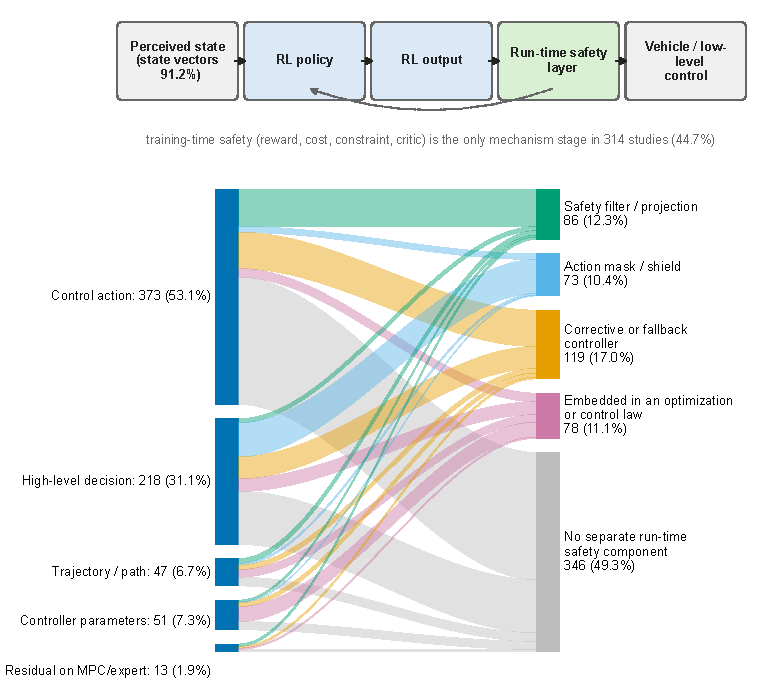
\includegraphics[width=\textwidth]{fig03_integration}
\caption{How the learned policy is coupled to safety. Top: the decision pipeline. Bottom: flows from what the RL policy outputs (left) to how a run-time safety component is attached (right); band widths are numbers of studies. Continuous control actions are mostly paired with filters or corrective controllers, high-level decisions with masks or embedded optimization.}\label{fig:integration}
\end{figure}

\subsection{Three integration patterns}
The cross-tabulation of outputs and safety attachments reveals three distinct patterns (Fig.~\ref{fig:integration}, Table~\ref{tab:control}).

\paragraph{Continuous control under a continuous safety layer.} When RL outputs the control action, the safety component is usually a filter (\nXActFilter{} of \nOutActN{} studies) or a corrective controller (\nXActCorrect). The filter is often a CBF-based quadratic program \citep{C0299,B1116} or a projection onto a feasible set \citep{B1658,B1169}. This pattern provides per-step safety for low-level control, as long as the filter's model and state estimate are valid.

\paragraph{Discrete decisions under masking or embedding.} When RL outputs a decision, safety is usually enforced by masking (\nXDecMask{} of \nOutDecN{} studies) or by a corrective rule or embedded optimization (\nXDecCorrEmb). The mask may be logic-based \citep{C0194}, prediction-based \citep{B0028}, reachability-based \citep{B0778}, chance-constrained \citep{B1430}, derived from a learned cost-to-go \citep{B1787}, or formally verified \citep{B0062}. The lower layer, typically an MPC or a CBF-based tracker \citep{B0776}, then executes the chosen maneuver safely.

\paragraph{RL tuning a certified controller.} In \nOutParamN{} studies, RL outputs the controller parameters, and in \nXParamEmbed{} studies, these parameters enter an optimization or control law. RL sets the MPC weights \citep{B0484,B1041}, CBF-MPC parameters \citep{A204}, CBF decay rate \citep{B1422}, MPC terminal cost \citep{B0577}, or gains of a stability-checked PID controller \citep{B1476}; tunes backstepping controllers whose state constraints are guaranteed by barrier Lyapunov functions \citep{B1508}; or replaces the online solver of the tube MPC \citep{B1137}. A related residual pattern allows RL to add a bounded correction to an MPC or expert command so that the model-based controller retains authority over hard constraints \citep{B1169,B1761}. These designs preserve the certificate intact by construction: the learned part only moves the controller within its safe envelope, which makes them attractive for certification-oriented work. However, the certificate must be feasible for every parameter that the policy can select. Studies have reported infeasible cases \citep{A204}, pre-verified a catalog of weights \citep{B0484}, or rejected gains that fail a stability check \citep{B1476}, and one study showed that a poorly chosen barrier parameter makes the same filter collide in every scenario \citep{B1422}.

%% BEGIN GENERATED tab07_control
\begin{sidewaystable}
\caption{Integration of RL with control-theoretic and formal safety components: what the learned policy outputs, how the safety component is attached, what the guarantee assumes, and the evidence reached}\label{tab:control}
\scriptsize
\setlength{\tabcolsep}{3pt}
\begin{tabularx}{\textheight}{@{}P{2.6cm} P{1.4cm} P{2.4cm} P{2.4cm} L P{0.8cm} P{0.6cm} P{3.0cm}@{}}
\toprule
Component & $n$ (\%) & RL output ($n$) & Attachment ($n$) & Main stated assumptions ($n$) & L4+ (\%) & Phys. & Example \\
\midrule
Control barrier function & 81 (11.5) & action (54); decision (13) & filter (41); embedded (19) & known or accurate dynamics model (36); bounded disturbance or error (24) & 44.4 & 9 & \citealp{B0327} \\
Lyapunov / CLF & 46 (6.6) & action (34); decision (4) & none (19); embedded (13) & known or accurate dynamics model (22); bounded disturbance or error (16) & 50.0 & 4 & \citealp{B1508} \\
CBF-CLF-QP / optimization layer & 28 (4.0) & action (14); decision (7) & filter (18); embedded (7) & known or accurate dynamics model (17); optimization feasibility (16) & 53.6 & 3 & \citealp{B1777} \\
MPC-RL hybrid & 104 (14.8) & action (29); decision (29) & embedded (55); filter (20) & predictable other road users (35); optimization feasibility (33) & 16.3 & 18 & \citealp{B0485} \\
Reachability / invariant sets & 39 (5.6) & action (21); decision (10) & corrective (9); embedded (8) & known or accurate dynamics model (13); predictable other road users (11) & 64.1 & 7 & \citealp{B0634} \\
Runtime assurance / fallback & 69 (9.8) & action (41); decision (20) & corrective (60); filter (4) & bounded disturbance or error (11); correct learned component or rule set (10) & 23.2 & 18 & \citealp{B0678} \\
\midrule
\multicolumn{8}{@{}>{\raggedright\arraybackslash}p{\dimexpr\textheight-1em\relax}@{}}{Any CBF, CLF, CBF-CLF-QP, MPC or reachability component: 220 (31.3); RL tunes a certified controller (parameters): 51 (7.3); RL adds a bounded residual: 13 (1.9).} \\
\botrule
\end{tabularx}
\footnotetext{Assumption themes are coded from the stated assumptions of studies at L3--L5 (Sect.~\ref{sec:integration}). Phys.: studies with physical or hardware-in-the-loop evidence. L3+/L4+: share of the row's studies whose highest substantiated evidence level is at least L3/L4. Example: a study matching the row, chosen by primary mechanism (where applicable), journal article in a JCR Q1/Q2 journal, highest safety-evidence level, quality score and recency; all studies are listed in the extraction database (Supplementary S3).}
\end{sidewaystable}
%% END GENERATED tab07_control

\subsection{What integration does and does not provide}
A run-time layer turns an empirical safety claim into a conditional, per-step claim. The condition, however, always lies outside the RL problem. Table~\ref{tab:control} lists the assumptions that studies state for each component, and Sect.~\ref{sec:discussion} analyses them across all studies at L3 or higher. The open question is therefore no longer \emph{whether} RL should be combined with control-theoretic safety, but \emph{which assumptions} the combination can afford in a real vehicle.



%% =====================================================================
\section{Autonomous-driving applications}\label{sec:apps}
%% =====================================================================
This section answers RQ4: where Safe RL is applied and how the strength of the safety evidence varies with the driving task.

\subsection{Tasks, road settings and traffic}
The most studied tasks are lane changing (\nTaskLcN; \nTaskLcP\%), car following and adaptive cruise control (\nTaskCfN; \nTaskCfP\%), intersections (\nTaskIntN; \nTaskIntP\%) and urban or route navigation (\nTaskNavN; \nTaskNavP\%). They are followed by collision avoidance (\nTaskCaN), merging (\nTaskMergeN), tactical decision making (\nTaskTdN), lane keeping (\nTaskLkN), motion planning (\nTaskMpN), and cooperative driving (\nTaskCoopN). Pedestrian interaction (\nTaskPedN; \nTaskPedP\%), emergency maneuvers (\nTaskEmgN), overtaking (\nTaskOvtN), platooning (\nTaskPltN), racing (\nTaskRaceN), end-to-end driving (\nTaskETwoeN; \nTaskETwoeP\%) and parking (\nTaskParkN) are under-represented (Fig.~\ref{fig:apps}, Table~\ref{tab:applications}). Highways (\nScenHwyN; \nScenHwyP\%), urban roads (\nScenUrbN; \nScenUrbP\%), and intersection areas (\nScenIntxN; \nScenIntxP\%) are the dominant settings.

Traffic surrounding the ego vehicle is usually simple. Other road users follow scripted models, such as the Intelligent Driver Model in \nTrafScriptedN{} studies (\nTrafScriptedP\%); replayed trajectories are used in \nTrafReplayN{}, and mixed autonomous and human-driven traffic models are used in \nTrafMixedN. Learning agents appear in only \nTrafLearnedN{} studies and human drivers in the loop in \nTrafHumanN{} \citep{B0240,B0761,B1370,B1765}. Safety is therefore mostly tested against road users who behave as the models predict, which is exactly the assumption that many guarantees rely on (Sect.~\ref{sec:discussion}).

\begin{figure}[!htbp]
\centering
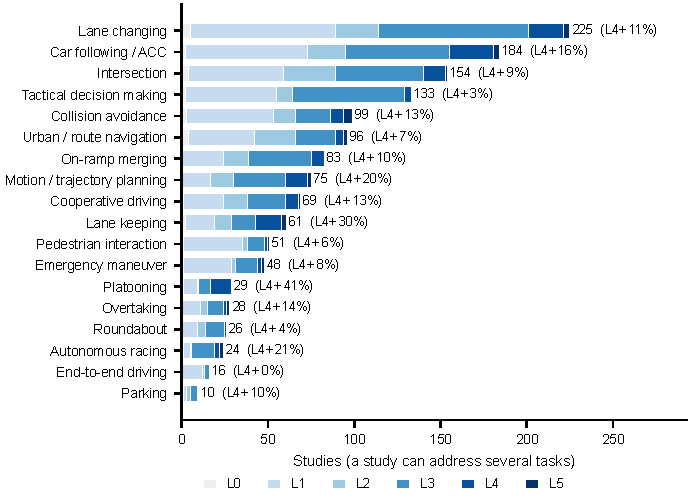
\includegraphics[width=0.9\textwidth]{fig06_applications}
\caption{Driving tasks addressed by the included studies, shaded by highest safety-evidence level; the label gives the number of studies and the share at L4 or above. Longitudinal and low-dimensional tasks (platooning, lane keeping) reach formal levels far more often than interactive tasks (urban navigation, pedestrian interaction, end-to-end driving).}\label{fig:apps}
\end{figure}

\subsection{Assurance follows task structure}
The strength of the safety evidence depends strongly on the task. Longitudinal and low-dimensional tasks reach formal levels most often: \nTaskPltLFourN{} of the \nTaskPltN{} platooning studies, \nTaskLkLFourN{} of the \nTaskLkN{} lane-keeping studies, and \nTaskCfLFourN{} of the \nTaskCfN{} car-following studies are at L4. Their dynamics are well modeled and suit barrier, MPC, and invariant-set methods. Interactive tasks are different. Urban navigation has only \nTaskNavLFourPlusN{} of \nTaskNavN{} studies at L4 or higher, pedestrian interaction \nTaskPedLFourPlusN{} of \nTaskPedN, and only \nTaskETwoeLThreePlusN{} of the \nTaskETwoeN{} end-to-end studies reach run-time enforcement, through a longitudinal speed cap \citep{B1640}, a rule that blocks dangerous lane changes \citep{C0051}, or safety-value rescoring of candidate trajectories \citep{C1049}. The tasks with the most complex interactions therefore have the weakest guarantees.

The choice of mechanism follows the level at which RL acts. Tactical decision making relies on run-time intervention (\nTaskTdMTwoN{} of \nTaskTdN{} studies used a cluster-M2 mechanism), consistent with masking discrete decisions. Urban navigation relies on objective shaping (\nTaskNavMOneN{} of \nTaskNavN) because the state and action spaces are too rich for simple rules or certificates.

%% BEGIN GENERATED tab04_applications
\begin{sidewaystable}
\caption{Application matrix: for each driving task, the dominant safety mechanisms, RL algorithms, simulators and safety metrics, and the strength of safety evidence}\label{tab:applications}
\scriptsize
\setlength{\tabcolsep}{3pt}
\begin{tabularx}{\textheight}{@{}P{2.3cm} P{1.4cm} P{2.6cm} P{2.7cm} P{2.3cm} L P{0.7cm} P{0.7cm} P{2.6cm}@{}}
\toprule
Task & $n$ (\%) & Mechanisms ($n$) & Algorithms ($n$) & Simulators ($n$) & Safety metrics ($n$) & L3+ & L4+ & Example \\
\midrule
Lane changing & 225 (32.1) & A (99); W (69); D (62) & DQN (44); PPO (32) & highway-env (71); SUMO (48) & collision (160); TTC (52) & 49.3 & 10.7 & \citealp{B0678} \\
Car following / ACC & 184 (26.2) & A (81); E (46); W (39) & DDPG (30); PPO (30) & custom (68); SUMO (39) & collision (86); TTC (65) & 48.4 & 15.8 & \citealp{B0896} \\
Intersection & 154 (21.9) & A (55); B (42); O (29) & PPO (27); SAC (24) & CARLA (51); SUMO (39) & collision (108); TTC (33) & 42.2 & 9.1 & \citealp{C0194} \\
Tactical decision making & 133 (18.9) & A (57); W (47); D (35) & DQN (32); Double DQN (20) & highway-env (35); custom (27) & collision (103); TTC (27) & 51.9 & 3.0 & \citealp{A096} \\
Collision avoidance & 99 (14.1) & A (47); F (20); Q (16) & PPO (20); SAC (17) & custom (32); CARLA (28) & collision (65); TTC (21) & 33.3 & 13.1 & \citealp{B0485} \\
Urban / route navigation & 96 (13.7) & A (34); B (31); V (18) & PPO (21); SAC (20) & CARLA (43); MetaDrive (21) & collision (57); violation (32) & 31.2 & 7.3 & \citealp{B0485} \\
On-ramp merging & 83 (11.8) & I (25); A (24); B (21) & PPO (16); SAC (11) & highway-env (28); SUMO (23) & collision (63); TTC (21) & 53.0 & 9.6 & \citealp{B1175} \\
Motion / trajectory planning & 75 (10.7) & I (26); B (17); A (17) & TD3 (9); PPO (8) & custom (29); CARLA (16) & collision (38); violation (12) & 60.0 & 20.0 & \citealp{A140} \\
Cooperative driving & 69 (9.8) & O (58); A (25); B (17) & MAPPO (12); PPO (9) & highway-env (19); CARLA (16) & collision (41); TTC (25) & 44.9 & 13.0 & \citealp{B0327} \\
Lane keeping & 61 (8.7) & G (17); K (15); B (13) & DDPG (16); PPO (10) & custom (21); Simulink (13) & collision (15); violation (14) & 52.5 & 29.5 & \citealp{A140} \\
Pedestrian interaction & 51 (7.3) & A (30); N (13); V (12) & PPO (16); SAC (11) & CARLA (19); custom (16) & collision (39); TTC (13) & 25.5 & 5.9 & \citealp{B0678} \\
Emergency maneuver & 48 (6.8) & A (26); I (14); O (7) & PPO (13); DDPG (12) & CARLA (17); custom (14) & collision (25); TTC (13) & 35.4 & 8.3 & \citealp{C0194} \\
Platooning & 29 (4.1) & G (11); E (9); K (9) & PPO (4); Actor-critic (4) & custom (12); SUMO (7) & gap/distance (14); TTC (8) & 65.5 & 41.4 & \citealp{B0750} \\
Overtaking & 28 (4.0) & A (14); I (9); W (7) & PPO (6); TD3 (4) & custom (8); CARLA (6) & collision (18); TTC (6) & 46.4 & 14.3 & \citealp{B0678} \\
Roundabout & 26 (3.7) & A (9); W (7); B (6) & DQN (6); PPO (5) & highway-env (10); CARLA (8) & collision (19); TTC (5) & 46.2 & 3.8 & \citealp{B1175} \\
Autonomous racing & 24 (3.4) & E (9); S (7); A (6) & PPO (10); SAC (5) & custom (13); TORCS (3) & collision (12); violation (5) & 75.0 & 20.8 & \citealp{B0757} \\
End-to-end driving & 16 (2.3) & A (8); L (4); W (3) & SAC (4); PPO (4) & CARLA (10); custom (2) & collision (10); off-road (4) & 18.8 & 0.0 & \citealp{C1049} \\
Parking & 10 (1.4) & R (3); O (3); I (3) & DQN (3); Hybrid-action constrained AC (1) & custom (5); highway-env (2) & collision (5); intervention (1) & 50.0 & 10.0 & \citealp{B1536} \\
\botrule
\end{tabularx}
\footnotetext{A study can address several tasks. Mechanism codes as in Table~\ref{tab:mechanisms}. L3+/L4+ in \%. L3+/L4+: share of the row's studies whose highest substantiated evidence level is at least L3/L4. Example: a study matching the row, chosen by primary mechanism (where applicable), journal article in a JCR Q1/Q2 journal, highest safety-evidence level, quality score and recency; all studies are listed in the extraction database (Supplementary S3).}
\end{sidewaystable}
%% END GENERATED tab04_applications

\subsection{Multi-agent and cooperative driving}
Multi-agent formulations, whose general training schemes are surveyed by \citet{gronauer2021madrl}, appear in \nMultiAgentN{} studies (\nMultiAgentP\%; Table~\ref{tab:multiagent}): \nAgCTDEN{} use centralized training with decentralized execution, \nAgDecN{} decentralized learning (often game-theoretic) and \nAgCenN{} a single centralized controller, typically for intersection management or platoons. Safety in these studies is most often enforced through constrained multi-agent policy optimization or shared CBF constraints between connected vehicles. Two features limit their transferability: many guarantees assume reliable vehicle-to-vehicle communication (Sect.~\ref{sec:discussion}), and only \nMultiAgentPhys{} multi-agent studies were tested on hardware, three of them on scaled vehicles \citep{B0882,B1443,B1778} and three on hardware-in-the-loop benches \citep{B1169,C1051,E019}.

%% BEGIN GENERATED tab09_multiagent
\begin{sidewaystable}
\caption{Multi-agent Safe RL for autonomous vehicles by training and execution architecture}\label{tab:multiagent}
\scriptsize
\setlength{\tabcolsep}{3pt}
\begin{tabularx}{\textheight}{@{}P{3.2cm} P{1.4cm} P{3.0cm} P{2.8cm} P{2.0cm} P{0.7cm} P{0.7cm} P{0.6cm} L@{}}
\toprule
Architecture & $n$ (\%) & Main tasks ($n$) & Algorithms ($n$) & Mechanisms ($n$) & Comm. & L3+ & Phys. & Example \\
\midrule
Centralized (one policy controls all agents) & 13 (1.9) & Cooperative driving (9); Intersection (6) & DDPG (3); TD3 (2) & A (7); B (4); W (4) & 6 & 38.5 & 1 & \citealp{B1786} \\
Centralized training, decentralized execution & 41 (5.8) & Cooperative driving (37); Intersection (19) & MAPPO (13); QMIX (5) & B (12); A (12); E (10) & 6 & 43.9 & 3 & \citealp{B0750} \\
Decentralized (independent or game-theoretic) & 44 (6.3) & Car following / ACC (20); Platooning (14) & PPO (8); DQN (6) & K (13); A (12); G (11) & 7 & 50.0 & 2 & \citealp{B0327} \\
\midrule
\multicolumn{9}{@{}>{\raggedright\arraybackslash}p{\dimexpr\textheight-1em\relax}@{}}{All multi-agent studies: 98 (14.0); at L4+: 16; with physical or HIL evidence: \citealp{B1443,B0882,B1169,B1778,C1051,E019}.} \\
\botrule
\end{tabularx}
\footnotetext{Comm.: studies whose safety claim states reliable V2V/V2I communication as an assumption. L3+ in \%. Phys.: physical or hardware-in-the-loop evidence. L3+/L4+: share of the row's studies whose highest substantiated evidence level is at least L3/L4. Example: a study matching the row, chosen by primary mechanism (where applicable), journal article in a JCR Q1/Q2 journal, highest safety-evidence level, quality score and recency; all studies are listed in the extraction database (Supplementary S3).}
\end{sidewaystable}
%% END GENERATED tab09_multiagent



%% =====================================================================
\section{Uncertainty, robustness and generalization}\label{sec:uncertainty}
%% =====================================================================
This section answers RQ6 (how uncertainty is handled) and RQ9 (how well methods generalize).

\subsection{Uncertainty (RQ6)}
In total, \nUncAnyN{} studies (\nUncAnyP\%) address at least one source of uncertainty (Table~\ref{tab:uncertainty}). Most of this uncertainty is of the easiest kind to simulate: stochastic traffic (\nUncStochN; \nUncStochP\%) and the intent of other road users (\nUncIntentN; \nUncIntentP\%). Model or dynamics mismatch is addressed in \nUncModelN{} studies (\nUncModelP\%), sensor noise or attacks on observations in \nUncSensN{} (\nUncSensP\%), distribution shift in \nUncDshiftN, partial observability and occlusion in \nUncPoN{} (\nUncPoP\%), prediction uncertainty in \nUncPredN, external disturbances in \nUncDistN{}, and adversarial agents in \nUncAdvN. Only \nUncExplicitN{} studies (\nUncExplicitP\%) explicitly estimate epistemic or aleatoric uncertainty, the two types distinguished in the deep-learning uncertainty literature \citep{gawlikowski2023uncertainty}, for example, with ensembles of critics \citep{A087}, Gaussian processes \citep{B0972}, distributional value functions \citep{C0438}, or Bayesian belief updates over driver intent \citep{B0878}.

The most effective use of these estimates is to couple them to a runtime mechanism: an uncertainty-triggered switch to a fallback controller \citep{A096,B1093}, uncertainty-adaptive barrier margins \citep{B0968}, chance constraints over noisy and occluded observations \citep{B1430}, or friction-dependent constraint tightening \citep{B1169,A053}. Without such coupling, an uncertainty estimate changes what the policy learns but not what the vehicle is allowed to do.

%% BEGIN GENERATED tab08_uncertainty
\begin{table}[!htbp]
\caption{Uncertainty addressed by the included studies, the mechanisms used to handle it, and how often generalization is tested alongside it}\label{tab:uncertainty}
\scriptsize
\setlength{\tabcolsep}{3pt}
\begin{tabularx}{\textwidth}{@{}P{3.0cm} P{1.3cm} P{1.9cm} P{0.9cm} P{0.7cm} L@{}}
\toprule
Uncertainty source & $n$ (\%) & Main mechanisms ($n$) & Gen.\ test (\%) & L3+ (\%) & Example \\
\midrule
Stochastic traffic & 211 (30.1) & D (47); I (31); L (29) & 69.7 & 45.5 & \citealp{B0678} \\
Intent of other road users & 158 (22.5) & N (35); D (27); I (26) & 76.6 & 42.4 & \citealp{B0678} \\
Model / dynamics mismatch & 87 (12.4) & K (38); E (28); F (27) & 77.0 & 70.1 & \citealp{A140} \\
Sensor noise or attack on observations & 73 (10.4) & K (29); N (26); E (16) & 91.8 & 43.8 & \citealp{A089} \\
External disturbance & 54 (7.7) & K (30); E (18); F (12) & 83.3 & 63.0 & \citealp{A140} \\
Partial observability, occlusion & 48 (6.8) & N (18); D (8); L (8) & 79.2 & 35.4 & \citealp{B0327} \\
Distribution shift & 48 (6.8) & N (18); S (15); L (8) & 93.8 & 37.5 & \citealp{B1093} \\
Epistemic (explicit estimate) & 43 (6.1) & N (41); S (17); L (13) & 79.1 & 58.1 & \citealp{B0972} \\
Adversarial agents or attacks & 42 (6.0) & K (38); E (6); F (6) & 90.5 & 26.2 & \citealp{B1777} \\
Prediction uncertainty & 40 (5.7) & N (20); Q (11); I (9) & 70.0 & 47.5 & \citealp{A089} \\
Aleatoric (explicit estimate) & 38 (5.4) & L (30); N (20); F (8) & 73.7 & 28.9 & \citealp{C0438} \\
\midrule
\multicolumn{6}{@{}>{\raggedright\arraybackslash}p{\dimexpr\textwidth-1em\relax}@{}}{No uncertainty addressed: 165 (23.5); any uncertainty: 537 (76.5); explicit epistemic or aleatoric estimate: 71 (10.1).} \\
\botrule
\end{tabularx}
\footnotetext{Mechanism codes as in Table~\ref{tab:mechanisms}, restricted to robustness, risk, uncertainty, certificate and run-time mechanisms. Gen.\ test: share of the row's studies with any generalization test. L3+/L4+: share of the row's studies whose highest substantiated evidence level is at least L3/L4. Example: a study matching the row, chosen by primary mechanism (where applicable), journal article in a JCR Q1/Q2 journal, highest safety-evidence level, quality score and recency; all studies are listed in the extraction database (Supplementary S3).}
\end{table}
%% END GENERATED tab08_uncertainty

\subsection{Generalization (RQ9)}
Some form of generalization is tested in \nGenAnyN{} studies (\nGenAnyP\%); the other \nGenNoneN{} (\nGenNoneP\%) test none. The most common tests were variations in traffic density (\nGenDensN), use of unseen scenarios (\nGenUnseenN), change in road geometry (\nGenGeomN), addition of disturbances (\nGenDistN), change in other agents (\nGenAgentsN), transfer from simulation to reality (\nGenSTworN), and introduction of a domain shift (\nGenDomainN). Generalization across vehicle dynamics (\nGenDynN; \nGenDynP\%) and weather or road friction (\nGenWeatherN; \nGenWeatherP\%) is rare, and no study tested transfer across traffic rules or countries. Generalization is also usually tested along a single axis at a time; therefore, it is not known how Safe RL policies behave when several conditions change simultaneously, as they do on real roads.



%% =====================================================================
\section{Simulation environments, benchmarks and safety metrics}\label{sec:eval}
%% =====================================================================
This section answers RQ7 (environments) and RQ8 (metrics). Simulators were coded only when they were used in a study's own experiments.

\subsection{Simulators and datasets (RQ7)}
Custom simulators are the most common environment (\nSimCustomN{} studies; \nSimCustomP\%), followed by CARLA \citep{dosovitskiy2017carla} (\nSimCARLAN; \nSimCARLAP\%), highway-env \citep{leurent2018highwayenv} (\nSimHWEnvN; \nSimHWEnvP\%), SUMO \citep{lopez2018sumo} (\nSimSUMON; \nSimSUMOP\%), MATLAB/Simulink (\nSimSimulinkN) and MetaDrive \citep{C0328} (\nSimMetaDriveN) (Table~\ref{tab:environments}). Datasets were used in \nDataAnyN{} studies (\nDataAnyP\%), for scenario generation, calibration of traffic models, replay, or offline training; NGSIM (\nDataNGSIM) and highD (\nDataHighD) are the most frequent public datasets, and \nDataOwn{} studies used data they collected themselves. The highest validation tier was low-fidelity simulation in \nTierSimLowN{} studies (\nTierSimLowP\%), high-fidelity simulation in \nTierSimHifiN{} (\nTierSimHifiP\%), and data-driven simulation in \nTierSimDataN{} (\nTierSimDataP\%).

Two consequences follow. First, because more than a quarter of the studies used a simulator built for the study, most results cannot be compared directly across studies. Second, the most popular open simulators have very different fidelity: highway-env and SUMO model vehicles kinematically and traffic at the level of lanes, whereas CARLA renders sensors and vehicle dynamics. A collision rate measured in one is not comparable with a collision rate measured in the other.

%% BEGIN GENERATED tab05_environments
\begin{table}[!htbp]
\caption{Simulation environments and datasets used in the experiments of the included studies}\label{tab:environments}
\scriptsize
\setlength{\tabcolsep}{3pt}
\begin{tabularx}{\textwidth}{@{}P{1.9cm} P{1.2cm} P{1.8cm} L P{0.6cm} P{3.1cm}@{}}
\toprule
Environment & $n$ (\%) & Most common highest tier & Main tasks ($n$) & Phys. & Example \\
\midrule
\multicolumn{6}{@{}>{\raggedright\arraybackslash}p{\dimexpr\textwidth-1em\relax}@{}}{\textit{Simulators (studies using each; a study can use several)}} \\
custom & 192 (27.4) & Low-fidelity simulation & Car following / ACC (68); Intersection (34) & 17 & \citealp{A089} \\
CARLA & 146 (20.8) & High-fidelity simulation & Intersection (51); Lane changing (44) & 10 & \citealp{B0678} \\
SUMO & 115 (16.4) & Low-fidelity simulation & Lane changing (48); Intersection (39) & 12 & \citealp{C0299} \\
highway-env & 114 (16.2) & Low-fidelity simulation & Lane changing (71); Tactical decision making (35) & 9 & \citealp{B0972} \\
Simulink & 54 (7.7) & Low-fidelity simulation & Car following / ACC (21); Lane keeping (13) & 7 & \citealp{B0896} \\
MetaDrive & 27 (3.8) & High-fidelity simulation & Urban / route navigation (21); Lane changing (4) & 3 & \citealp{B0485} \\
CarSim & 22 (3.1) & High-fidelity simulation & Emergency maneuver (7); Lane keeping (7) & 7 & \citealp{B0896} \\
PreScan & 13 (1.9) & High-fidelity simulation & Lane changing (3); Car following / ACC (3) & 4 & \citealp{B1793} \\
SMARTS & 12 (1.7) & Low-fidelity simulation & Intersection (6); On-ramp merging (6) & 0 & \citealp{B1640} \\
Unity & 12 (1.7) & High-fidelity simulation & Collision avoidance (5); Lane changing (5) & 0 & \citealp{B0246} \\
CommonRoad & 10 (1.4) & Data-driven simulation & Lane changing (9); Car following / ACC (5) & 0 & \citealp{C0299} \\
other named simulators & 55 (7.8) & \multicolumn{4}{p{8.2cm}}{Safety Gym, TORCS, Flow, TruckSim, Learn-to-Race (Arrival simulator), Webots, OpenDS, NS3, and others} \\
\midrule
\multicolumn{6}{@{}>{\raggedright\arraybackslash}p{\dimexpr\textwidth-1em\relax}@{}}{\textit{Datasets (used for scenarios, calibration, replay or offline training)}} \\
own collected data & 62 (8.8) & -- & Car following / ACC (19); Urban / route navigation (15) & 14 & \citealp{B0678} \\
NGSIM & 40 (5.7) & -- & Car following / ACC (24); Lane changing (11) & 0 & \citealp{A089} \\
highD & 22 (3.1) & -- & Car following / ACC (14); Lane changing (13) & 0 & \citealp{C0299} \\
other datasets & 34 (4.8) & \multicolumn{4}{p{8.2cm}}{inD, Waymo Open, nuPlan, INTERACTION, Lyft Level 5 Motion Prediction, nuScenes, DSRL, rounD, and others} \\
\midrule
\multicolumn{6}{@{}>{\raggedright\arraybackslash}p{\dimexpr\textwidth-1em\relax}@{}}{Any dataset: 150 (21.4); custom simulator: 192 (27.4); scripted surrounding traffic: 428 (61.0).} \\
\botrule
\end{tabularx}
\footnotetext{Phys.: studies with physical or hardware-in-the-loop evidence. Only simulators actually used in the experiments were coded (mentions in related work were ignored). Simulators and datasets used by fewer than ten studies are grouped. Example: a study matching the row, chosen by primary mechanism (where applicable), journal article in a JCR Q1/Q2 journal, highest safety-evidence level, quality score and recency; all studies are listed in the extraction database (Supplementary S3).}
\end{table}
%% END GENERATED tab05_environments

\subsection{Safety metrics (RQ8)}
Collision rate or count is by far the most common safety metric (\nMetCollN{} studies; \nMetCollP\%), followed by TTC (\nMetTtcN), constraint violations (\nMetViolN) and safety-layer interventions (\nMetIntervN) (Table~\ref{tab:metrics}). Post-encroachment time (\nMetPetN) and explicit risk measures (\nMetRiskN) are rare. Safety measurement is narrow: \nSafeMetNoneN{} studies (\nSafeMetNoneP\%) report no safety metric at all, \nSafeMetOneN{} (\nSafeMetOneP\%) report exactly one, and collision is the only safety metric in \nCollOnlyN{} (\nCollOnlyP\%). Performance quantities are often presented as evidence of safety: the success rate (\nMetSuccN{} studies) and reward (\nMetRewN) are reported more frequently than any safety metric except collisions.

Statistical reporting is weak. Only \nStatsFullN{} studies (\nStatsFullP\%) report variability together with significance tests or confidence intervals, \nStatsPartialN{} (\nStatsPartialP\%) report variability only, and \nStatsNoneN{} (\nStatsNoneP\%) report neither. A small number of test episodes cannot show that a policy is safe with respect to rare events, yet ``zero collisions in $N$ episodes'' is a common claim. Studies that address rare events directly are few: rare-event verification \citep{B1403}, safety-critical scenario generation \citep{B1806}, tail-risk cost models \citep{B1798}, and harm-weighted rare-event costs \citep{B1046}. One study stands out for scale, evaluating over 42{,}000\,km of stochastic simulated traffic calibrated on naturalistic data \citep{B1333}.

%% BEGIN GENERATED tab06_metrics
\begin{table}[!htbp]
\caption{Evaluation metrics reported by the included studies, grouped by what they measure}\label{tab:metrics}
\footnotesize
\setlength{\tabcolsep}{3pt}
\begin{tabularx}{\textwidth}{@{}P{1.8cm} L P{2.0cm}@{}}
\toprule
Category & Metric & Studies, $n$ (\%) \\
\midrule
safety & collision rate or count & 410 (58.4) \\
safety & time to collision (TTC) & 160 (22.8) \\
safety & constraint or safety-cost violations & 103 (14.7) \\
safety & headway, gap or minimum distance & 96 (13.7) \\
safety & safety-layer interventions or takeovers & 59 (8.4) \\
safety & off-road or lane departure & 38 (5.4) \\
safety & explicit risk measure & 24 (3.4) \\
safety & traffic-rule violations & 21 (3.0) \\
safety & post-encroachment time (PET) & 9 (1.3) \\
safety & unsafe-action frequency & 2 (0.3) \\
task & success or completion rate & 302 (43.0) \\
efficiency & average speed & 174 (24.8) \\
efficiency & travel time or time to goal & 167 (23.8) \\
efficiency & energy or fuel & 50 (7.1) \\
efficiency & traffic throughput & 38 (5.4) \\
comfort & comfort index & 138 (19.7) \\
comfort & jerk & 126 (17.9) \\
comfort & acceleration & 33 (4.7) \\
tracking & lateral/longitudinal tracking error & 110 (15.7) \\
learning & episode return & 218 (31.1) \\
learning & sample efficiency / convergence & 54 (7.7) \\
computation & computation time & 82 (11.7) \\
composite & driving score (e.g.\ CARLA leaderboard) & 8 (1.1) \\
composite & generalization score & 1 (0.1) \\
\midrule
\multicolumn{3}{@{}>{\raggedright\arraybackslash}p{\dimexpr\textwidth-1em\relax}@{}}{Studies with no safety metric: 92 (13.1); exactly one: 354 (50.4); collision as the only safety metric: 214 (30.5).} \\
\multicolumn{3}{@{}>{\raggedright\arraybackslash}p{\dimexpr\textwidth-1em\relax}@{}}{Statistical reporting: full (variance and tests) 105 (15.0); partial (variance only) 280 (39.9); none 317 (45.2).} \\
\botrule
\end{tabularx}
\footnotetext{A study usually reports several metrics. Reward and success are performance quantities and are not counted as safety metrics.}
\end{table}
%% END GENERATED tab06_metrics



%% =====================================================================
\section{Explainability and trust}\label{sec:xai}
%% =====================================================================
This section answers RQ10. Explainability is rarely a research target in this literature. Only \nXaiVisN{} studies (\nXaiVisP\%) produced explanations and inspected them, mostly attention visualizations \citep{B0257} or saliency maps \citep{C0281}, and occasionally feature attributions or analyses of risk and world-model variables \citep{B0678,B0640}. A further \nXaiDesignN{} studies (\nXaiDesignP\%) claimed that their method was interpretable by design, for example, through verified policy structures \citep{B0157}, reward machines \citep{B0432}, interpretable safety models such as RSS \citep{B1409}, or fuzzy rule tables \citep{B0976}; however, they did not evaluate the claim. No study evaluated explanations with users, drivers, or safety engineers, although black-box multi-agent policies are recognized as an obstacle to trustworthy deployment in high-stakes settings \citep{sheng2026xmarl}.

The most practical source of interpretability in this corpus is architectural, rather than post hoc. A rule-based monitor, a barrier-function override, or a model-based fallback behaves predictably and can be inspected and verified independently of the learned policy \citep{B1533,B1333}. This is a plausible route to trustworthy Safe RL, but it remains an argument rather than an established result because none of these claims have been tested with people.

%% =====================================================================
\section{Sim-to-real validation and reproducibility}\label{sec:simreal}
%% =====================================================================
This section answers RQ11 (how often methods progress beyond simulation) and RQ12 (reproducibility).

\subsection{Beyond simulation (RQ11)}
Of the \nIncluded{} studies, \nSimOnlyN{} (\nSimOnlyP\%) are simulation-only. Of the \nPhysN{} studies with physical or hardware-in-the-loop evidence, \nTierHILN{} used hardware-in-the-loop or processor-in-the-loop setups, \nTierScaledN{} scaled vehicles or robots, \nTierClosedN{} full-size vehicles on closed courses, and \nTierRoadN{} roads (Table~\ref{tab:simreal}). No study reported a deployed system, that is, one in series production or operational service. The \nTierRoadN{} road studies were themselves heterogeneous: two used campus roads \citep{B0716,B1569}, two reported proprietary fleet results only in summary \citep{B0517,B0658}, three from one integrated decision-and-control line of work drove real urban intersections, one of them with virtual surrounding traffic from a digital twin \citep{B1271,C0315,C0992}, two drove an RL policy on public highways or mixed road segments with empirical (L1) evidence only \citep{C0381,C0720}, and one ran a CBF-supervised RL cruise controller on a production vehicle in live urban traffic \citep{B0761}. Physical tests are typically short and slow, for example, at 12--18\,km/h on a closed segment \citep{A140}, at up to 4\,m/s on a 1/10-scale car \citep{B0757}, or as a straight run on a low-speed chassis \citep{B1409}.

Physical validation and strong guarantees rarely meet (Fig.~\ref{fig:validation}). Only \nPhysLFive{} of the \nPhysN{} studies with physical or hardware-in-the-loop evidence reached L5; the others sat at L0 (\nPhysLZero), L1 (\nPhysLOne), L2 (\nPhysLTwo), L3 (\nPhysLThree), or L4 (\nPhysLFour). Many of them relied on human, teacher, or fallback supervision, or on training-time constraints, rather than on a certified run-time layer. One proving-ground study completed every ISO 3888-2 double-lane-change test, but nothing in its architecture enforced safety at run time \citep{B1474}.

\begin{figure}[!htbp]
\centering
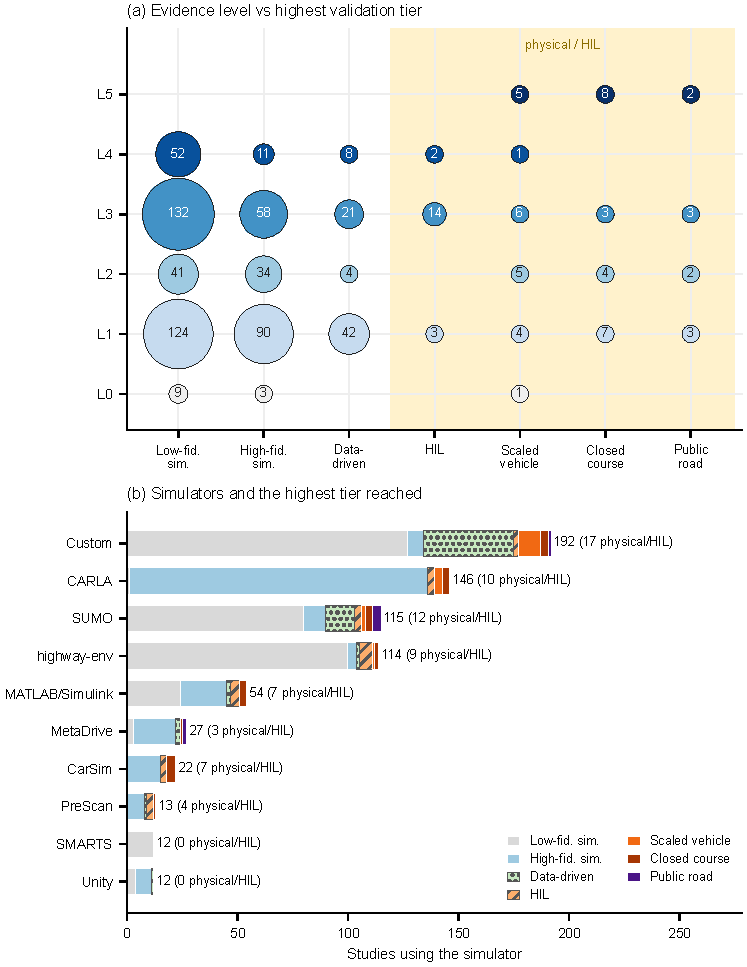
\includegraphics[width=\textwidth]{fig08_validation}
\caption{Validation landscape. (a) Highest substantiated safety-evidence level against the highest validation tier reached; bubble area and label give the number of studies. Formal (L4) results concentrate in low-fidelity simulation, while physical studies rarely carry formal properties (the assurance--realism inversion). (b) The ten most used simulators, split by the highest validation tier reached by the studies that use them.}\label{fig:validation}
\end{figure}

%% BEGIN GENERATED tab10_simreal
\begin{table}[!htbp]
\caption{Studies that progress beyond simulation, by highest validation tier and safety-evidence level}\label{tab:simreal}
\scriptsize
\setlength{\tabcolsep}{3pt}
\begin{tabularx}{\textwidth}{@{}P{2.0cm} P{0.4cm} P{2.0cm} P{2.8cm} L@{}}
\toprule
Highest tier & $n$ & Evidence levels & Studies at L5 & Other studies (examples) \\
\midrule
Hardware-in-the-loop & 19 & L1 3, L3 14, L4 2 & -- & \citealp{B1777,B0575} \\
Scaled vehicle & 22 & L0 1, L1 4, L2 5, L3 6, L4 1, L5 5 & \citealp{B1230,B1270,B0757,B0882,E060} & \citealp{B1409,B1778} \\
Closed course (full size) & 22 & L1 7, L2 4, L3 3, L5 8 & \citealp{B0028,A140,B0444,A074,B0485,B0507,B0678,B0896} & \citealp{B1445,B0640} \\
Public road & 10 & L1 3, L2 2, L3 3, L5 2 & \citealp{B0716,B0761} & \citealp{C0315,C0992} \\
\midrule
\multicolumn{5}{@{}>{\raggedright\arraybackslash}p{\dimexpr\textwidth-1em\relax}@{}}{Simulation only: 629 (89.6) (low-fidelity 358, high-fidelity 196, data-driven 75); deployment: 0.} \\
\botrule
\end{tabularx}
\footnotetext{L5 requires run-time or formal safety (L3/L4) together with a physical test that reports a safety analysis (Sect.~\ref{sec:levels}).}
\end{table}
%% END GENERATED tab10_simreal

\subsection{Reproducibility (RQ12)}
Code is released by \nCodeN{} studies (\nCodeP\%), and this share has not improved over time (\nPerOneCodeP\%, \nPerTwoCodeP\%, \nPerThreeCodeP\% and \nPerFourCodeP\% in the four periods; Table~\ref{tab:repro}). Data were released by \nDataN{} studies (\nDataP\%). Hyperparameters were fully reported in \nHypFullN{} studies (\nHypFullP\%), random seeds in \nSeedsN{} (\nSeedsP\%), compute in \nComputeN{} (\nComputeP\%) and a complete evaluation protocol in \nProtocolN{} (\nProtocolP\%). Comparisons are often weak: \nBaseNsrlN{} studies (\nBaseNsrlP\%) compare their method with an RL baseline without safety mechanisms, but only \nBaseSrlN{} (\nBaseSrlP\%) with another Safe RL method and \nBaseClassN{} (\nBaseClassP\%) with a classical controller. Many reported safety improvements are therefore measured against an unconstrained baseline, the weakest possible comparison. Statistical practices from the wider RL community, such as reporting interval estimates across seeds \citep{agarwal2021precipice}, are rarely adopted \citep{B1692}.

%% BEGIN GENERATED tab11_repro
\begin{table}[!htbp]
\caption{Reproducibility of the included studies, overall and by publication period}\label{tab:repro}
\footnotesize
\setlength{\tabcolsep}{3pt}
\begin{tabularx}{\textwidth}{@{}L P{1.6cm} P{1.4cm} P{1.4cm} P{1.4cm} P{1.4cm}@{}}
\toprule
Item & All, $n$ (\%) & 2016--2020 (\%, $n$=62) & 2021--2022 (\%, $n$=124) & 2023--2024 (\%, $n$=213) & 2025--2026 (\%, $n$=303) \\
\midrule
Code released & 83 (11.8) & 12.9 & 10.5 & 12.2 & 11.9 \\
Data released & 70 (10.0) & 11.3 & 12.1 & 8.0 & 10.2 \\
Hyperparameters fully reported & 423 (60.3) & 37.1 & 54.0 & 60.1 & 67.7 \\
Hyperparameters partly reported & 211 (30.1) & 48.4 & 33.1 & 31.0 & 24.4 \\
Random seeds reported & 158 (22.5) & 12.9 & 13.7 & 17.8 & 31.4 \\
Compute reported & 329 (46.9) & 24.2 & 29.8 & 51.6 & 55.1 \\
Full evaluation protocol & 404 (57.5) & 40.3 & 50.8 & 51.2 & 68.3 \\
Statistical reporting (variance and tests) & 105 (15.0) & 12.9 & 15.3 & 12.7 & 16.8 \\
Compared with another Safe RL method & 144 (20.5) & 8.1 & 11.3 & 19.7 & 27.4 \\
Compared with a classical controller & 287 (40.9) & 37.1 & 37.1 & 46.0 & 39.6 \\
\botrule
\end{tabularx}
\footnotetext{Seeds reported: the number of seeds or their use is stated.}
\end{table}
%% END GENERATED tab11_repro



%% =====================================================================
\section{The Safe RL deployment-readiness chain}\label{sec:framework}
%% =====================================================================

Sections~\ref{sec:taxonomy}--\ref{sec:simreal} answer the research questions one at a time. However, for deployment, what matters is how they connect: which RL approach is combined with which safety mechanism, what guarantee that combination actually delivers, in which driving application, under what evaluation, and how close the result is to a deployable system. Catalogs of methods, which most earlier surveys provide, cannot answer this. We therefore introduce a review-derived framework that links the evidence along one chain:
\begin{center}
\emph{Safe RL approach} $\rightarrow$ \emph{safety mechanism} $\rightarrow$ \emph{safety guarantee} $\rightarrow$ \emph{AV application} $\rightarrow$ \emph{evaluation} $\rightarrow$ \emph{deployment readiness}.
\end{center}
Every link is coded for every included study, and the chain combines these codes by fixed rules. The judgment lies in the coding of each link, chiefly the evidence level (Sect.~\ref{sec:levels}), not in the combination. What the chain adds to the separate tables is the joint view: it shows, for each family of mechanisms, whether the evidence stops at the guarantee or at the evaluation, and it separates studies that took a policy onto hardware without a run-time guarantee from those that carried one there.

\subsection{Definition}
The first, second and fourth links are the RL approach, the primary safety mechanism and the driving tasks recorded in the extraction database (Sects.~\ref{sec:taxonomy} and~\ref{sec:apps}). The \emph{guarantee} link condenses the evidence levels of Sect.~\ref{sec:levels} into five classes: G0 safety asserted only, G1 empirical, G2 constraint satisfied in expectation, G3 run-time enforced, and G4 formal under stated assumptions. The \emph{evaluation} link condenses the validation tiers into E1 low-fidelity simulation, E2 high-fidelity or data-driven simulation, E3 hardware-in-the-loop or scaled vehicle, E4 full-size vehicle on a closed course or road, and E5 deployment. \emph{Deployment readiness} combines the two:
\begin{itemize}
\item \textbf{Low}: an empirical or expectation-level guarantee (G0--G2) shown only in simulation (E1--E2);
\item \textbf{Low--Medium}: a run-time or formal guarantee (G3--G4) shown only in simulation, or a weaker guarantee with hardware evidence (E3--E4);
\item \textbf{Medium}: a run-time or formal guarantee on hardware-in-the-loop or a scaled vehicle (E3);
\item \textbf{Medium--High}: a run-time or formal guarantee on a full-size vehicle (E4);
\item \textbf{High}: evidence from deployment or certification (E5).
\end{itemize}
The scale is deliberately simple and conservative. It asks two questions that any safety engineer would ask of a Safe RL result: \emph{does anything stop the policy from acting unsafely at run time?} and \emph{has that been shown on a real vehicle?} It does not judge whether a method is promising, only how far its evidence has traveled.

\subsection{Where the chain breaks}
Only \nRdyMediumPlusN{} studies (\nRdyMediumPlusP\%) reach Medium readiness or higher: \nRdyMediumN{} at Medium and \nRdyMediumHighN{} at Medium--High. Of the rest, \nRdyLowN{} (\nRdyLowP\%) are at Low and \nRdyLowMediumN{} (\nRdyLowMediumP\%) at Low--Medium, and none reaches High (Fig.~\ref{fig:chain}, Table~\ref{tab:framework}). Following the chain from left to right shows two distinct bottlenecks.

\paragraph{The guarantee bottleneck.} Objective-shaping mechanisms rarely produce a runtime or formal guarantee; only \nFamRewardGThreeP\% of the studies whose primary mechanism is reward shaping, \nFamRiskGThreeP\% of risk-sensitive studies, and \nFamConstrainedGThreeP\% of constrained-RL studies reach G3 or higher. Therefore, their readiness remains at Low, regardless of how they are evaluated; no reward-shaping or risk-sensitive study reaches Medium. Learning-paradigm extensions (offline, hierarchical, human-in-the-loop, and foundation-model-assisted RL) behave similarly, with only \nFamParadigmGThreeP\% at G3 or higher.

\paragraph{The evaluation bottleneck.} Run-time and certificate mechanisms solve the guarantee problem: \nFamFilterGThreeP\% of safety-filter studies, \nFamShieldGThreeP\% of shield and rule-based studies, \nFamBarrierGThreeP\% of barrier-certificate studies, and \nFamFormalGThreeP\% of reachability and formal-verification studies reach G3 or higher. Yet, only \nFamFilterMedPlusP\%, \nFamShieldMedPlusP\%, \nFamBarrierMedPlusP\%, and \nFamFormalMedPlusP\% of them, respectively, reach Medium readiness, because \nGuarRuntimeSimOnlyP\% of all studies with a run-time or formal guarantee are evaluated only in simulation. The chain does not break at the method; it breaks at the evaluation.

\paragraph{Where the chain holds.} Two families convert guarantees into readiness most often: runtime assurance (\nFamRTAMedPlusP\% at Medium or higher) and MPC hybrids (\nFamMPCMedPlusP\%). Both place a model-based component with explicit authority over the vehicle beside the learned policy, which is the architecture that automotive engineers already know how to test. The Medium--High studies illustrate the end of the chain: a CBF filter supervising an RL cruise controller on a production vehicle in public traffic \citep{B0761}, constrained RL with an MPC shield on a real off-road vehicle \citep{B0896}, MPC-expert takeover on a full-size vehicle \citep{A140}, and shielded lane changing on a real vehicle \citep{B0444}. Conversely, \nPhysWeakGuarN{} studies took a policy onto hardware without a run-time or formal guarantee, which raised their evaluation but not their readiness.

\begin{figure}[!htbp]
\centering
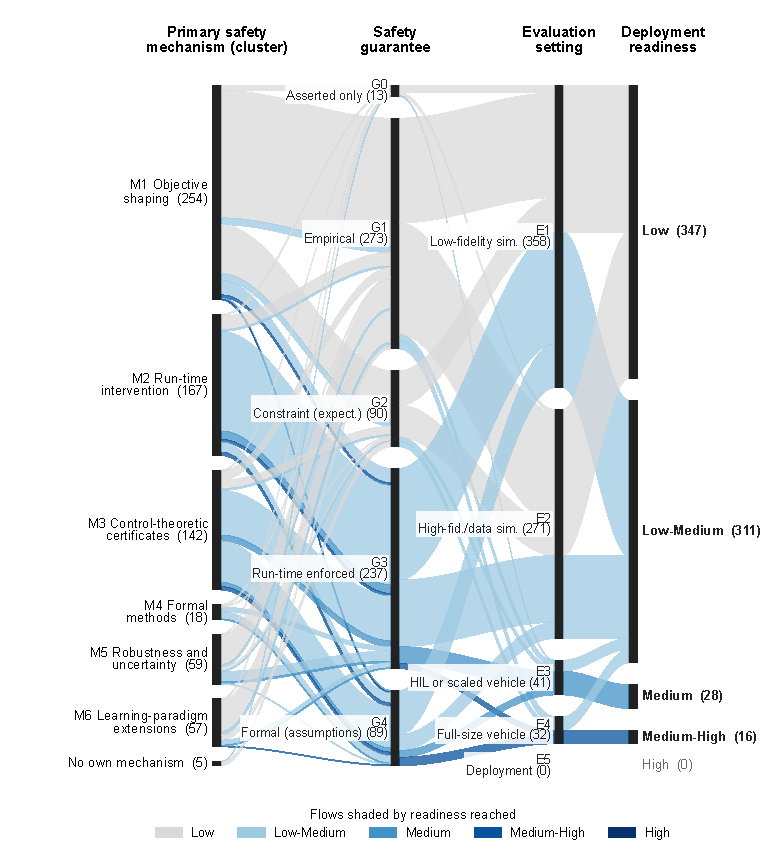
\includegraphics[width=\textwidth]{fig11_readiness_chain}
\caption{The Safe RL deployment-readiness chain computed for all \nIncluded{} included studies: primary safety mechanism (grouped into the clusters M1--M6 of Fig.~\ref{fig:taxonomy}), safety guarantee class (G0--G4), evaluation setting (E1--E5) and resulting deployment readiness. Band widths are numbers of studies; bands are shaded by the readiness the studies finally reach. Run-time and certificate mechanisms pass the guarantee stage but most stop at simulation; no study reaches High readiness.}\label{fig:chain}
\end{figure}

%% BEGIN GENERATED tab15_framework
\begin{sidewaystable}
\caption{The Safe RL deployment-readiness chain: for each family of primary safety mechanism, the typical RL approach, the safety guarantee it reaches, the AV applications, the evaluation setting and the resulting deployment readiness (review-derived; computed from the coded evidence of every study)}\label{tab:framework}
\scriptsize
\setlength{\tabcolsep}{3pt}
\begin{tabularx}{\textheight}{@{}P{2.3cm} P{0.5cm} P{2.4cm} P{2.3cm} P{3.1cm} P{1.0cm} P{1.6cm} P{0.8cm} L@{}}
\toprule
Safety mechanism (primary) & $n$ & Safe RL approach ($n$) & Typical guarantee & Main AV applications ($n$) & Sim.\ only / phys. & Readiness L / LM / M / MH & Med.+ (\%) & Example \\
\midrule
Reward shaping & 135 & PPO (40); DDPG (28) & Empirical; G3+ 1.5\% & Car following / ACC (47); Lane changing (35) & 129 / 6 & 127/8/0/0 & 0.0 & \citealp{C0381} \\
Constrained RL / safety critic & 84 & SAC-Lagrangian (12); PPO-Lagrangian (12) & Constraint in expectation; G3+ 22.6\% & Lane changing (25); Intersection (24) & 72 / 12 & 59/19/2/4 & 7.1 & \citealp{B0896} \\
Risk-sensitive RL & 35 & SAC (8); DQN (6) & Empirical; G3+ 5.7\% & Lane changing (11); Intersection (11) & 31 / 4 & 29/6/0/0 & 0.0 & \citealp{B1175} \\
Shield, mask or rule-based intervention & 92 & DQN (21); PPO (14) & Run-time enforced; G3+ 83.7\% & Lane changing (55); Tactical decision making (32) & 85 / 7 & 13/74/2/3 & 5.4 & \citealp{C0822} \\
Safety filter & 44 & SAC (10); TD3 (9) & Run-time enforced; G3+ 95.5\% & Car following / ACC (16); Lane changing (9) & 41 / 3 & 2/39/2/1 & 6.8 & \citealp{B1445} \\
Runtime assurance & 31 & PPO (7); SAC (7) & Run-time enforced; G3+ 90.3\% & Lane changing (11); Tactical decision making (7) & 22 / 9 & 3/19/6/3 & 29.0 & \citealp{B0678} \\
Barrier / Lyapunov certificate (CBF, CLF, CBF-CLF-QP) & 80 & SAC (15); PPO (15) & Formal under assumptions; G3+ 81.2\% & Car following / ACC (31); Collision avoidance (18) & 72 / 8 & 13/61/4/2 & 7.5 & \citealp{A074} \\
MPC hybrid & 48 & SAC (10); DQN (8) & Run-time enforced; G3+ 87.5\% & Motion / trajectory planning (14); Car following / ACC (11) & 40 / 8 & 6/34/7/1 & 16.7 & \citealp{B0485} \\
Reachability / formal verification & 32 & DQN (11); PPO (6) & Formal under assumptions; G3+ 81.2\% & Lane changing (12); Car following / ACC (9) & 29 / 3 & 6/23/2/1 & 9.4 & \citealp{B0507} \\
Robust / uncertainty-aware RL & 59 & PPO (11); SAC (8) & Empirical; G3+ 25.4\% & Lane changing (22); Tactical decision making (20) & 53 / 6 & 40/17/2/0 & 3.4 & \citealp{B1093} \\
Learning-paradigm extension & 57 & PPO (8); SAC (8) & Empirical; G3+ 14.0\% & Urban / route navigation (19); Lane changing (17) & 51 / 6 & 45/10/1/1 & 3.5 & \citealp{B0716} \\
\midrule
\multicolumn{9}{@{}>{\raggedright\arraybackslash}p{\dimexpr\textheight-1em\relax}@{}}{All studies: readiness Low 347, Low--Medium 311, Medium 28, Medium--High 16, High 0.} \\
\botrule
\end{tabularx}
\footnotetext{Guarantee classes: G0 asserted only, G1 empirical, G2 constraint satisfied in expectation, G3 run-time enforced, G4 formal under stated assumptions (from evidence levels L0--L5, with L5 counted as G4). Readiness: Low = empirical or expectation-level guarantee (G0--G2), simulation only (E1--E2); Low--Medium = run-time or formal guarantee (G3--G4) in simulation only, or a weaker guarantee with hardware evidence (E3--E4); Medium = run-time or formal guarantee (G3--G4) on hardware-in-the-loop or a scaled vehicle (E3); Medium--High = run-time or formal guarantee (G3--G4) on a full-size vehicle, closed course or road (E4); High = deployment or certification evidence (E5). Readiness distribution lists Low/Low--Medium/Medium/Medium--High; no study reaches High. Sim.\ only / phys.: studies evaluated only in simulation / with physical or hardware-in-the-loop evidence; Med.+: share at Medium readiness or higher. Example: highest readiness, then a JCR Q1/Q2 journal article, evidence level, quality score and recency.}
\end{sidewaystable}
%% END GENERATED tab15_framework

\paragraph{Readiness by application.} Readiness also differs by driving task (Table~\ref{tab:readinesstasks}). Lane keeping (\nTaskLkMedPlusN{} of \nTaskLkN{} studies at Medium or higher), car following (\nTaskCfMedPlusN{} of \nTaskCfN), lane changing (\nTaskLcMedPlusN{} of \nTaskLcN), and collision avoidance (\nTaskCaMedPlusN{} of \nTaskCaN) have the most studies that have traveled furthest, whereas only \nTaskMergeMedPlusN{} of the \nTaskMergeN{} merging studies \citep[a hardware-in-the-loop test of MPC-based cooperative merging;][]{E019}, none of the \nTaskETwoeN{} end-to-end studies, and only \nTaskPedMedPlusN{} of the \nTaskPedN{} pedestrian-interaction studies reach Medium. Interactive tasks with other road users are therefore not only the hardest to certify (Sect.~\ref{sec:apps}) but also the least validated beyond simulation.

%% BEGIN GENERATED tab16_readiness_tasks
\begin{table}[!htbp]
\caption{Deployment readiness by driving task (review-derived readiness classes, see Table~\ref{tab:framework})}\label{tab:readinesstasks}
\scriptsize
\setlength{\tabcolsep}{3pt}
\begin{tabularx}{\textwidth}{@{}P{3.0cm} P{0.5cm} P{0.6cm} P{0.6cm} P{0.6cm} P{0.6cm} P{1.4cm} L@{}}
\toprule
Task & $n$ & Low & Low--Med. & Med. & Med.--High & Medium or higher (\%) & Highest-readiness examples \\
\midrule
Lane changing & 225 & 104 & 109 & 8 & 4 & 5.3 & \citealp{B0678} \\
Car following / ACC & 184 & 91 & 82 & 8 & 3 & 6.0 & \citealp{B0896} \\
Intersection & 154 & 80 & 65 & 6 & 3 & 5.8 & \citealp{B1445} \\
Tactical decision making & 133 & 61 & 69 & 3 & 0 & 2.3 & \citealp{A096} \\
Collision avoidance & 99 & 55 & 37 & 4 & 3 & 7.1 & \citealp{B0485} \\
Urban / route navigation & 96 & 60 & 29 & 2 & 5 & 7.3 & \citealp{B0485} \\
On-ramp merging & 83 & 38 & 44 & 1 & 0 & 1.2 & \citealp{E019} \\
Motion / trajectory planning & 75 & 24 & 43 & 4 & 4 & 10.7 & \citealp{A140} \\
Cooperative driving & 69 & 37 & 28 & 4 & 0 & 5.8 & \citealp{B1778} \\
Lane keeping & 61 & 24 & 25 & 9 & 3 & 19.7 & \citealp{A140} \\
Pedestrian interaction & 51 & 36 & 14 & 0 & 1 & 2.0 & \citealp{B0678} \\
Emergency maneuver & 48 & 27 & 16 & 4 & 1 & 10.4 & \citealp{B0507} \\
Platooning & 29 & 9 & 19 & 1 & 0 & 3.4 & \citealp{B1169} \\
Overtaking & 28 & 11 & 14 & 1 & 2 & 10.7 & \citealp{B0678} \\
Roundabout & 26 & 14 & 10 & 2 & 0 & 7.7 & \citealp{C1043} \\
Autonomous racing & 24 & 5 & 13 & 6 & 0 & 25.0 & \citealp{B0757} \\
End-to-end driving & 16 & 12 & 4 & 0 & 0 & 0.0 & \citealp{C1049} \\
Parking & 10 & 5 & 4 & 0 & 1 & 10.0 & \citealp{C0822} \\
\botrule
\end{tabularx}
\footnotetext{A study can address several tasks.}
\end{table}
%% END GENERATED tab16_readiness_tasks

\subsection{Using the chain}
The chain is intended as a reporting and assessment template for future work as well as a lens on past work. A new Safe RL study for autonomous vehicles can state its position on each link: the RL approach, the mechanism that acts at runtime (if any), the guarantee class with its assumptions, the driving application, the evaluation setting, and the resulting readiness. Doing so would make clear what a result does and does not show, and it identifies the next step for each family. For objective-shaping methods, the next step is a runtime layer; for runtime and certificate methods, it is evaluation on hardware with the same layer and its assumption checks; and for every family, it is eventually deployment or certification evidence, which no study yet provides. These steps correspond directly to the core research problems and roadmap in Sect.~\ref{sec:gaps}.

%% =====================================================================
\section{Discussion}\label{sec:discussion}
%% =====================================================================
This section draws together the findings of Sects.~\ref{sec:taxonomy}--\ref{sec:framework} under three cross-cutting themes: the difference between optimizing performance and assuring safety, the reasons why Safe RL remains largely simulation-bound, and the place of Safe RL in the autonomous-driving stack.

\subsection{Performance optimization versus safety assurance}
The review-derived evidence levels separate \emph{showing} that a policy behaved safely from \emph{ensuring} that it will. Across the corpus, \nLevLZeroN{} studies (\nLevLZeroP\%) asserted safety without evaluating it (L0), \nLevLOneN{} (\nLevLOneP\%) evaluated it only empirically (L1), \nLevLTwoN{} (\nLevLTwoP\%) reported the satisfaction of explicit constraints (L2), \nLevLThreeN{} (\nLevLThreeP\%) enforced safety at run time (L3), \nLevLFourN{} (\nLevLFourP\%) established formal properties under stated assumptions (L4), and \nLevLFiveN{} (\nLevLFiveP\%) carried run-time or formal safety onto a physical vehicle with a safety analysis (L5). Three findings follow.

\paragraph{Most safety claims rest on performance-style evidence.} Almost half of the studies (\nClaimEmpOnlyP\%) make only an empirical safety claim, and the evidence is usually a collision rate measured over a modest number of episodes in one simulator (Sect.~\ref{sec:eval}). Higher reward, higher success rate, or fewer collisions in a set of test episodes show that a policy performs well in the tested conditions; they do not show that it is safe in conditions that were not tested. Studies that move beyond this, by enforcing safety at runtime or proving a property, are the minority.

\paragraph{The assurance--realism inversion.} The strongest guarantees are demonstrated in the least realistic settings (Fig.~\ref{fig:validation}a). Of the \nLevLFourN{} studies at L4, \nLFourSimN{} were validated only in simulation, and \nLFourLowN{} of them (\nLFourLowP\%) only in low-fidelity simulators. Conversely, of the \nPhysN{} studies with physical or hardware-in-the-loop evidence, only \nPhysLFive{} reached L5. A property proven for a kinematic model in a two-dimensional simulator does not automatically hold on a vehicle, and real-vehicle studies rarely carry formal properties with them. This inversion is the central tension of the field.

\paragraph{What the guarantees assume.} Of the \nAsmBaseN{} studies at L3 or higher, \nAsmStatedN{} state the assumptions behind their safety claim. The most frequent are predictable other road users, for example constant-velocity or worst-case motion models (\nAsmOthersN; \nAsmOthersP\%); a known or accurate dynamics model, often control-affine or kinematic (\nAsmModelN; \nAsmModelP\%); bounded disturbances or errors (\nAsmBoundedN; \nAsmBoundedP\%); feasibility of the optimization layer (\nAsmFeasibleN; \nAsmFeasibleP\%); correctness of a learned component or rule set (\nAsmLearnedN; \nAsmLearnedP\%); perfect perception or privileged simulator state (\nAsmPerceptionN; \nAsmPerceptionP\%); and reliable communication (\nAsmCommN; \nAsmCommP\%). These are precisely the places where a real driving system is weakest: the intent of other drivers, model mismatch, and perception noise.

Several studies have shown how fragile the guarantees are. A CBF-filtered adaptive cruise controller reached collision rates of 11--31\% once its state input was attacked \citep{A164}. The verified LiDAR-based controllers discussed in Sect.~\ref{sec:formal} crashed when sensor faults fell outside the verified model \citep{B1230}. The public-road test of a CBF-filtered cruise controller measured clear errors in its double-integrator model, although the filter still prevented time-gap violations \citep{B0761}. Formal verification of neural car controllers revealed inconsistencies between the specification and simulator \citep{B0937}, and CBF filters failed under model mismatch and moving obstacles until a disturbance observer and a predictive barrier were added \citep{A035}.

Robust variants relax these assumptions with disturbance observers \citep{A035}, Gaussian-process estimates of friction or model error \citep{A053,B0972}, conformal prediction of state errors \citep{B0750}, robust barriers under bounded observation errors or attacks \citep{B1777}, tube MPC and robust predictive filters \citep{A089,B1536}, and chance constraints over occlusion \citep{B1430}. Each of these, however, replaces one assumption with a bound that must itself be validated.

\subsection{Why Safe RL remains largely simulation-bound}
Almost nine in ten studies never leave simulation. The evidence points to six reasons, which together form the deployment gap.
\begin{enumerate}
\item \emph{Exploration risk.} Learning by trial and error on a vehicle is unsafe. The real-world studies either learn under human supervision \citep{B0716,B1569}, transfer a policy trained in simulation without further learning \citep{B0882,B0757}, or run a policy trained elsewhere under a run-time supervisor \citep{B0761}. Proposals to learn directly on the vehicle behind a backup controller \citep{B0972} have so far been tested only in simulation.
\item \emph{Assumption mismatch.} Guarantees rely on models, predictions, and state estimates that a real vehicle does not provide exactly, and the two studies that measured this on hardware found it directly \citep{B0761,B1230}.
\item \emph{Rare events.} Safety at the level of road statistics cannot be demonstrated with hundreds of test episodes \citep{kalra2016driving}, and rare-event testing is uncommon in the corpus (Sect.~\ref{sec:eval}).
\item \emph{Computation and timing.} Only \nTierHILN{} studies test on hardware-in-the-loop or embedded targets \citep{B0575,B1093}. Timing claims made on desktop hardware \citep{B1658} remain unverified on automotive processors.
\item \emph{Certification.} Only one study maps its evidence to an automotive standard: it builds a safety case following the AMLAS guidance \citep{hawkins2021amlas}, with an ISO~26262 hazard analysis, for an RL collision-avoidance component of a scaled vehicle, but it reuses earlier experimental evidence without new testing \citep{B1443}. A full-text search for safety standards found them otherwise only in related-work discussions \citep{B0381}, in statements that place them out of scope \citep{B1793}, in claims without a compliance analysis \citep{B1658,B1041}, or in plans for future work \citep{B0987,B1787}.
\item \emph{Reproducibility and tooling.} Custom simulators and unreleased code (Sect.~\ref{sec:simreal}) make independent re-validation, the first step toward any certification, difficult.
\end{enumerate}
These reasons interact. Because guarantees depend on assumptions that cannot be checked in simulation, and because rare events cannot be sampled sufficiently in short tests, neither simulation nor small-scale physical testing alone can establish deployment-level safety. What is missing is a pipeline that carries the \emph{same} safety layer and its assumption checks from simulation to the vehicle.

\subsection{Mapping Safe RL onto the AV safety stack}
Mapping the studies onto the layers of an autonomous-driving stack shows where Safe RL contributes and where it does not. Safe RL concentrates on control (\nStackCtrlN{} studies; \nStackCtrlP\%), decision making (\nStackDecN; \nStackDecP\%), and safety supervision (\nStackSupervN; \nStackSupervP\%). Planning is addressed in \nStackPlanN{} studies (\nStackPlanP\%), whereas perception (\nStackPercN; \nStackPercP\%) and prediction (\nStackPredN; \nStackPredP\%) are rarely addressed. Runtime assurance as an explicit architectural layer appears in \nStackRtaN{} studies, although fallback mechanisms of some kind appear in \nMechSN. The layers where real-world hazards originate, perception and prediction, are therefore the ones Safe RL addresses least; yet they are exactly the layers whose outputs the safety guarantees assume to be correct. This mismatch explains much of the assurance--realism inversion: guarantees are proved for the planning and control layers, given perfect inputs from layers that are not part of the safety argument.
%% =====================================================================
\section{Research gaps and future directions}\label{sec:gaps}
%% =====================================================================
This section answers RQ13 (unresolved problems) and RQ14 (research directions supported by the evidence). Each gap is retained only because the extraction database supports it, and each is quantified by one indicator (Fig.~\ref{fig:gaps}, Table~\ref{tab:gaps}).

\subsection{Research gaps (RQ13)}
Fifteen gaps emerge from the analysis. They concern the transfer of safety to vehicles (G1, G2, G15), the assumptions behind guarantees (G3, G6), the kind of safety being guaranteed (G9) and measured (G4), the realism of the scenarios (G8), the place of Safe RL in the driving stack (G12), the measurement infrastructure of the field (G5, G7, G10, G11) and the assurance and explainability of learned policies (G13, G14).

\subsection{Core research problems}\label{sec:problems}
The fifteen gaps reduce to eight core problems, ordered by how directly they block real-world deployment.

\paragraph{P1. Carrying a safety guarantee from simulation onto the vehicle (G1, G2, G15).} This is the evaluation bottleneck of the readiness chain (Sect.~\ref{sec:framework}). Guarantees live in simple simulators, while hardware studies rarely carry a certified layer, and the single public-road test of a certified filter around an RL policy covers longitudinal control only \citep{B0761}. The open question is how the same safety layer, with the same assumptions, can be validated at every stage from simulation to hardware-in-the-loop, closed course and road, so that the guarantee and its evidence travel together. A convincing answer would report the assumption checks, intervention rates and violation statistics at each stage, on target hardware and in real time.

\paragraph{P2. Guarantees that survive imperfect perception, prediction and models (G3, G6, G12).} The stronger claims assume predictable road users, accurate models and perfect state, and attacks, model error and sensor faults have been shown to break or strain them \citep{B0761,B1230}. Certificates such as CBFs, MPC, reachable sets and shields need to be built from calibrated bounds on perception, prediction and model error, and the calibration itself needs validation. A convincing answer would show coverage of the uncertainty bounds on real data and safety under sensor noise, occlusion and adversarial input, not only under the nominal model.

\paragraph{P3. From expected-cost safety to tail-risk and rare-event safety (G4, G9).} Constrained RL is the second most common mechanism but bounds only expected cost, and claims of zero collisions in a finite number of episodes usually come without statistics. Policies need to be trained and certified against state-wise or tail-risk constraints, and rare-event safety needs to be estimated with statistical confidence, for example with failure-rate estimates and confidence bounds from targeted generation of safety-critical scenarios.

\paragraph{P4. Safety in interactive, multi-agent and vulnerable-road-user traffic (G8, G3).} Surrounding traffic is scripted in most studies, pedestrian interaction is rare, and multi-agent methods assume reliable communication. Safety needs to be certified when other agents react, deviate from models or fail to communicate, and when pedestrians and cyclists are involved, with harm-weighted outcomes.

\paragraph{P5. Safe end-to-end and perception-in-the-loop learning (G12, G6).} Nearly all policies act on already-perceived state vectors, and end-to-end studies almost never enforce safety at run time. It is open where the safety layer should sit when the policy acts on raw sensor input, and which state estimate it can trust; a convincing answer would place a run-time layer on uncertainty-aware perception outputs and evaluate it in closed loop with realistic sensors.

\paragraph{P6. A measurement science for Safe RL in driving (G4, G5, G7, G10, G11).} Custom simulators, single safety metrics, weak baselines, missing statistics and unreleased code make safety claims hard to compare or reproduce. The field needs shared scenarios, multiple safety metrics (violations, TTC and post-encroachment-time distributions, intervention rates), mandatory Safe RL and classical baselines, statistical reporting and released code and scenarios.

\paragraph{P7. Assurance evidence that certification and people can use (G13, G14, G15).} One study builds a safety case and none feeds new test evidence into one; formal methods have declined and are rarely tested physically; and no study tests explanations with users. Safe RL evidence (levels, assumptions, test results, monitor behavior) needs to be structured into safety arguments aligned with ISO~26262 and ISO~21448 \citep{iso26262,iso21448}, with compositional verification of the safety layer rather than of the whole policy, and made inspectable by engineers, regulators and drivers.

\paragraph{P8. Keeping new learning paradigms inside the safety envelope (trends in Sect.~\ref{sec:biblio}).} Offline, foundation-model-assisted, human-in-the-loop and hierarchical methods are growing but mostly inherit empirical or constraint-level evidence, and human or language-model guidance usually ends with training \citep{B1745}. The open question is how these paradigms can improve performance and coverage without becoming the component on which the safety argument depends; a convincing answer would bound the new component by an independent run-time safety layer and show that the bound holds under distribution shift.

\subsection{Future research directions (RQ14)}
Table~\ref{tab:roadmap} and Fig.~\ref{fig:roadmap} translate the core problems into eleven directions over three horizons. The analysis thus runs from 15 measured gaps (G1--G15) through eight core problems (P1--P8) to 11 directions (R1--R11), so that every direction can be traced back to the evidence. The horizons reflect what each direction requires: short-term directions require only a change in practice with existing tools, medium-term directions require new methods, and long-term directions require new assurance practices and, ultimately, acceptance by regulators. Each direction builds on studies that have already pointed the way.

\paragraph{Short term: benchmarks and reporting.} The cheapest and most urgent step is a common safety evaluation protocol (R1): several safety metrics reported together with confidence intervals, violations during both training and testing, and intervention rates for filtered policies, compared against Safe RL and classical baselines in shared environments. It should come with a reproducibility minimum (R2) and with explicit reporting of each study's position on the deployment-readiness chain, including the evidence level reached and every assumption a guarantee needs (R3), so that readers can see what a result does and does not show. Together, R1--R3 amount to a minimum reporting standard. We suggest that every Safe RL study for autonomous vehicles report at least: (i) safety violations during training and during testing, separately; (ii) more than one safety metric, for example collisions, constraint violations, and TTC or PET distributions, with confidence intervals over seeds and episodes; (iii) intervention rates for any filter, shield, or fallback; (iv) a comparison with at least one Safe RL baseline and one classical controller; (v) the number of seeds and test episodes; (vi) the evidence level reached (L0--L5) and every assumption the guarantee needs; (vii) the validation tier; and (viii) the code, configurations, and scenario files. Today, only \nBaseSrlP\% of studies compare their method with another Safe RL method and \nCodeP\% release code (Table~\ref{tab:repro}).

\paragraph{Medium term: methods that relax assumptions.} Barrier and MPC layers should take their margins from calibrated uncertainty through conformal, Gaussian-process, observer-based, robust, or chance-constrained bounds and be tested against noise and attacks (R4). Epistemic uncertainty should trigger verified fallbacks evaluated on embedded hardware (R5). Interactive safety requires reactive or human traffic, communication loss, and harm-weighted pedestrian scenarios (R6). Expected-cost constraints should give way to state-wise and tail-risk constraints evaluated with scenarios generated against the current policy (R7). Finally, staged pipelines should carry one safety layer from high-fidelity simulation through hardware-in-the-loop and closed courses to supervised road trials (R8).

\paragraph{Long term: assurance and certification.} Verification should target the safety layer and monitor its assumptions at runtime rather than attempt to verify the entire learned policy (R9). The resulting evidence should be organized into certification-oriented safety cases in which the RL policy is a performance component bounded by an assured supervisor (R10), the architecture that already produces most of the L3--L5 evidence in this corpus. New paradigms such as offline learning, world models, and foundation models should operate inside, not instead of, this safety envelope (R11). Explanations need the same scrutiny: the transparency that a monitor or fallback offers should be evaluated with drivers, engineers, and safety assessors rather than assumed, because no study in the corpus has done so (Sect.~\ref{sec:xai}; R11).

\begin{figure}[!htbp]
\centering
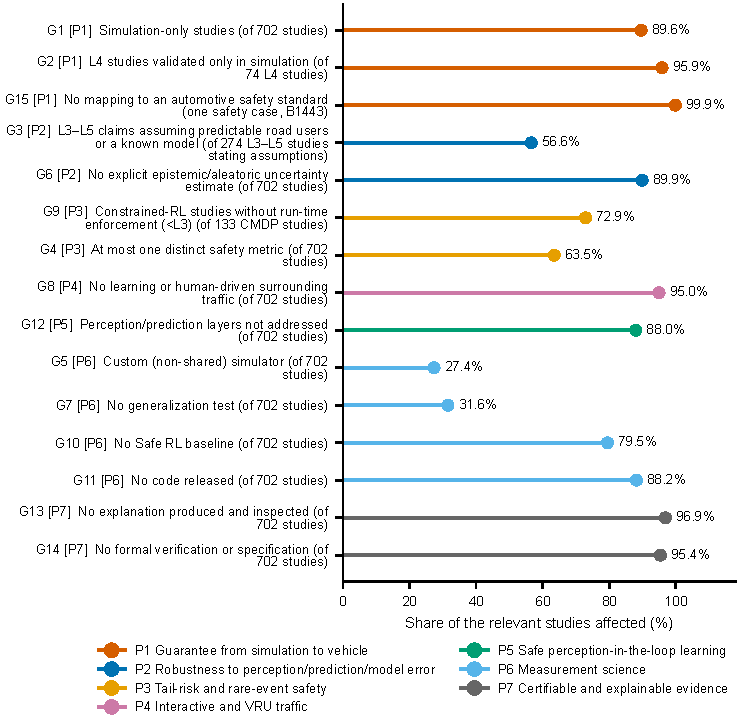
\includegraphics[width=\textwidth]{fig09_gaps}
\caption{Research-gap landscape. Each gap (G1--G15) is quantified by one indicator computed from the extraction database: the share of the relevant studies affected (denominator in parentheses). The core research problem (P1--P7) each gap feeds is given in square brackets and by color; P8 is supported by trend evidence (Fig.~\ref{fig:evolution}) rather than a single indicator.}\label{fig:gaps}
\end{figure}
%% BEGIN GENERATED tab13_gaps
\begin{sidewaystable}
\caption{Research gaps supported by the evidence, the indicator that quantifies each gap, and the core research problem it feeds}\label{tab:gaps}
\scriptsize
\setlength{\tabcolsep}{3pt}
\begin{tabularx}{\textheight}{@{}P{0.5cm} P{4.2cm} L P{0.6cm} P{4.4cm}@{}}
\toprule
ID & Gap & Evidence (computed from the extraction database) & Prob. & Illustrative study \\
\midrule
G1 & Simulation-to-reality and deployment gap & Simulation-only studies: 89.6\% (of 702 studies); 10 public-road studies, 0 deployments & P1 & \citealp{B0761} \\
G2 & Strong guarantees only in simple simulators (assurance--realism inversion) & L4 studies validated only in simulation: 95.9\% (of 74 L4 studies); 15 studies at L5 & P1 & \citealp{B0757} \\
G15 & Weak link to safety standards and target-hardware evidence & No mapping to an automotive safety standard: 99.9\% (of 702 studies); 19 HIL studies; one safety case & P1 & \citealp{B1443} \\
G3 & Guarantees conditional on idealized prediction, models and perception & L3--L5 claims assuming predictable road users or a known model: 56.6\% (of 274 L3--L5 studies stating assumptions); fragility shown under attack, model error and sensor faults & P2 & \citealp{A164} \\
G6 & Limited uncertainty modeling, especially perception & No explicit epistemic/aleatoric uncertainty estimate: 89.9\% (of 702 studies); sensor uncertainty in 10.4\% & P2 & \citealp{B0750} \\
G9 & Expected-value constraints do not cover rare catastrophic events & Constrained-RL studies without run-time enforcement ($<$L3): 72.9\% (of 133 CMDP studies); rare-event or tail-risk methods in a handful of studies & P3 & \citealp{B0658} \\
G4 & Narrow and inconsistent safety metrics; weak statistics & At most one distinct safety metric: 63.5\% (of 702 studies); collision the only safety metric in 30.5\%; no statistics in 45.2\% & P3 & \citealp{B1403} \\
G8 & Interactive and vulnerable-road-user scenarios under-served & No learning or human-driven surrounding traffic: 95.0\% (of 702 studies); pedestrian interaction in 7.3\% & P4 & \citealp{B1046} \\
G12 & Safe RL absent from perception and prediction; end-to-end safety unaddressed & Perception/prediction layers not addressed: 88.0\% (of 702 studies); image input in 4.6\%; end-to-end studies at L3+: 3 & P5 & \citealp{B1640} \\
G5 & No shared benchmark or evaluation protocol & Custom (non-shared) simulator: 27.4\% (of 702 studies); scripted traffic in 61.0\% & P6 & \citealp{B0930} \\
G7 & Narrow generalization testing & No generalization test: 31.6\% (of 702 studies); weather/friction 10, vehicle dynamics 25, traffic rules 0 & P6 & \citealp{B0754} \\
G10 & Weak comparative baselines & No Safe RL baseline: 79.5\% (of 702 studies); classical-controller baseline in 40.9\% & P6 & \citealp{B0308} \\
G11 & Reproducibility not improving & No code released: 88.2\% (of 702 studies); seeds reported in 22.5\% & P6 & \citealp{B1692} \\
G13 & Explainability unexamined & No explanation produced and inspected: 96.9\% (of 702 studies); no study evaluates explanations with users & P7 & \citealp{B0268} \\
G14 & Formal methods not scaling to learned driving policies & No formal verification or specification: 95.4\% (of 702 studies); formal-methods share 17.7\% / 5.6\% / 2.8\% / 2.6\% across the four periods & P7 & \citealp{B0937} \\
\botrule
\end{tabularx}
\footnotetext{Indicators as in Fig.~\ref{fig:gaps}. Problems P1--P8 are defined in Sect.~\ref{sec:gaps}. The illustrative study documents the gap or points to a partial answer.}
\end{sidewaystable}
%% END GENERATED tab13_gaps
%% BEGIN GENERATED tab14_roadmap
\begin{table}[!htbp]
\caption{Future research directions, each linked to the core problems (P) and gaps (G) it addresses and to studies that already point the way}\label{tab:roadmap}
\scriptsize
\setlength{\tabcolsep}{3pt}
\begin{tabularx}{\textwidth}{@{}P{0.9cm} P{0.5cm} L P{1.9cm} P{2.6cm}@{}}
\toprule
Horizon & ID & Direction & Addresses & Building on \\
\midrule
Short & R1 & Common safety evaluation protocol: several safety metrics with confidence intervals, violations during training and testing, TTC/PET distributions and intervention rates; Safe RL and classical baselines & P6; G4, G5, G10 & \citealp{B0308} \\
Short & R2 & Reproducibility minimum: code, seeds, simulator configurations and scenario files released with every safety claim & P6; G11 & \citealp{B0847} \\
Short & R3 & Report the safety-evidence level reached and every assumption the guarantee needs & P1, P2; G2, G3 & \citealp{B1116} \\
Medium & R4 & Perception- and prediction-aware certificates whose margins come from calibrated uncertainty (conformal, Gaussian-process, observer, robust or chance-constrained bounds), tested against noise and attacks & P2, P5; G3, G6, G12 & \citealp{B0750} \\
Medium & R5 & Uncertainty-triggered runtime assurance with verified fallbacks, evaluated on embedded hardware & P1, P2; G1, G6 & \citealp{A096} \\
Medium & R6 & Interactive, multi-agent and vulnerable-road-user safety with reactive or human traffic, communication loss and harm-weighted costs & P4; G8 & \citealp{B0882} \\
Medium & R7 & State-wise and tail-risk constraints and safety-critical scenario generation against the current policy & P3; G9 & \citealp{B0658} \\
Medium & R8 & Staged sim-to-real pipelines that carry the same safety layer from high-fidelity simulation through HIL and closed courses to supervised road trials & P1; G1, G7 & \citealp{A140} \\
Long & R9 & Compositional verification of the safety layer and run-time monitoring of its assumptions & P7; G14 & \citealp{B0937} \\
Long & R10 & Certification-oriented safety cases that map RL evidence to automotive standards, with the policy bounded by an assured supervisor & P7; G15 & \citealp{B1443} \\
Long & R11 & Offline, world-model, human-guided and foundation-model methods kept inside an independent safety envelope; explanations evaluated with users & P8; G13 & \citealp{B1584} \\
\botrule
\end{tabularx}
\end{table}
%% END GENERATED tab14_roadmap
\begin{figure}[!htbp]
\centering
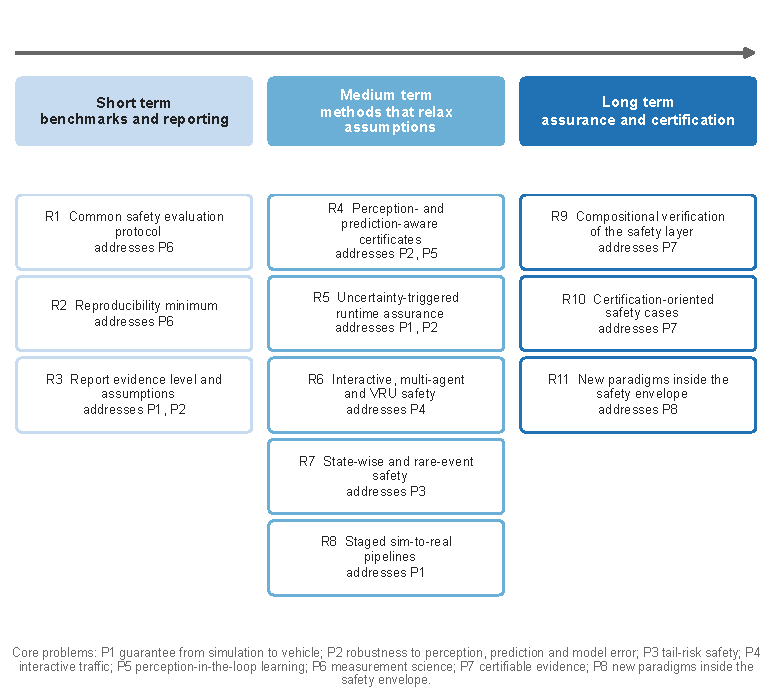
\includegraphics[width=\textwidth]{fig10_roadmap}
\caption{Research roadmap. Directions R1--R11 are grouped by horizon and linked to the core problems they address (details and building-block studies in Table~\ref{tab:roadmap}).}\label{fig:roadmap}
\end{figure}


%% =====================================================================
\section{Threats to validity}\label{sec:validity}
%% =====================================================================
\paragraph{Construct validity.} The search relied on vocabulary. Citation searching showed that none of the \nScopeCitN{} studies it added used Safe RL terminology in its title, and these studies relied on empirical evidence more often than database-search studies (Sect.~\ref{sec:biblio}). Studies that combined RL with a safety mechanism without using our terms may still have been missed, although the second query, which combines RL with control-theoretic and formal-method terms, and the title-only query reduce this risk, and the final strategy retrieved 36 of 38 known-relevant seed studies. ``Safety'' itself is defined operationally through the eligibility criteria; studies in which safety played no role in the method or evaluation were excluded, which may have removed some relevant performance-oriented work. The evidence levels and mechanism clusters are frameworks proposed by this review, not established standards, and other groupings are possible.

\paragraph{Internal validity.} Screening, extraction, and quality scoring were carried out with AI assistance under a written protocol and codebook, with validation scripts that enforce controlled vocabularies and documented coding rules. In the screening-consistency sample, initial agreement was low ($\kappa=\nConsKappaFwd$), mainly because the second screener first applied a broader reading of the criteria; all disagreements were resolved against the written criteria, and no record changed status (Sect.~\ref{sec:dedup}). The low agreement nonetheless shows that the explicit-safety criterion (IC2) involves judgment: a looser reading would add RL driving studies that handle safety only implicitly, for example through collision penalties, and would shift the corpus further toward empirical evidence, as the search-scope comparison in Sect.~\ref{sec:biblio} also suggests. Coding conventions for borderline cases are documented in the codebook (Supplementary S3), so that individual codes can be traced and re-examined. Coding of assumption themes uses transparent text rules and is approximate, and quality items partly overlap with the evaluation practices whose prevalence we report, which makes some sensitivity comparisons circular.

\paragraph{External validity.} Only English-language publications were included, and subscription databases were not queried directly, although their content is indexed by OpenAlex. Of the \nSoughtAll{} reports sought, \nNotRetrievedAll{} (\nNotRetrieved{} of \nSought{} from the database search and \nCitNotRetrieved{} of \nCitSought{} from citation searching) could not be retrieved: in the database search mainly from small publishers and from journals and book series outside the institutional subscription, and in citation searching mainly from publisher platforms that could not be accessed (ScienceDirect, SAGE, and Taylor \& Francis). Within the database search, the retrieval rounds differed in code release but hardly in safety evidence (Sect.~\ref{sec:biblio}), so the missing database reports are unlikely to change the main conclusions. The missing citation-search reports, if they resemble the retrieved ones, would add mostly empirical (L1) studies and slightly lower the shares of stronger evidence; this cannot be verified. Preprints were included when technically complete, and 2026 is a partial year. Citation searching added \nCitOnlyIncluded{} studies that the database queries missed, which shows the limits of keyword search in this field. Because only one round was run, and the citation search screened only records that passed an automated keyword filter, some relevant studies may still be missing.

\paragraph{Reporting bias.} The evidence is likely to be affected by reporting bias. Studies choose the scenarios, baselines, and metrics they report; failures of safety methods are rarely published; and claims of zero collisions in a finite number of episodes are far more common than reports of failure cases. Shares that depend on reported outcomes, such as the empirical safety of a method, are therefore more likely to overstate safety than to understate it. The structural findings (which mechanisms are used, whether they act at runtime, how and where they are evaluated, and whether the code is released) do not depend on the reported outcomes and are less affected.

\paragraph{Conclusion validity.} No meta-analysis was possible because the scenarios, metrics, and safety definitions differed across studies. All quantitative statements are therefore descriptive frequencies and cross-tabulations, generated by a script from the extraction database and released with this article.

%% =====================================================================
\section{Conclusion}\label{sec:conclusion}
%% =====================================================================
This review asked how Safe RL has been developed, evaluated and applied to make autonomous vehicles safer, and what separates it from real-world deployment. Across \nIncluded{} studies, the answer has three parts.

First, the field has converged on combining learning with explicit safety machinery, and it is this machinery, not the RL algorithm, that protects the vehicle. Reward shaping and expected-cost constraints, the most common mechanisms, rarely enforce safety on individual actions. Run-time interventions and control-theoretic certificates (shields, safety filters, runtime assurance, control barrier functions, MPC, and reachable sets) can, but only when they act at runtime: \nRtMechBelowP\% of the studies that use such a mechanism apply it only during training or leave it unevaluated, so having a safety layer is not the same as using one. Increasingly, these mechanisms allow RL to choose decisions, parameters, or bounded residuals, while a model-based layer maintains authority over hard constraints.

Second, the strength of safety evidence lags behind the sophistication of the methods used. In total, \nSimOnlyP\% of studies are simulation-only, nearly all formal guarantees are demonstrated only in simulation, most of them in low-fidelity simulators, and only \nLevLFiveN{} studies combine run-time or formal safety with a physical test and a safety analysis. The guarantees typically assume predictable road users, accurate models, and perfect perception, which are conditions that a real vehicle cannot provide. Safety is usually measured using a single metric, often without statistics, and code is rarely released. The deployment-readiness chain shows where the evidence stops: only \nRdyMediumPlusN{} studies reach Medium readiness or higher, and none reaches deployment. Objective-shaping methods stop at the guarantee; run-time and certificate methods stop at the evaluation; and runtime assurance and MPC hybrids travel the furthest.

Third, the evidence points to a clear path. In the short term, the field requires a shared safety evaluation protocol and explicit reporting of evidence levels and assumptions. In the medium term, it requires certificates built from calibrated uncertainty, uncertainty-triggered fallbacks, interactive and rare-event testing, and staged sim-to-real pipelines that carry one safety layer onto the vehicle. In the long term, it requires verification of the safety layer and its assumptions, and certification-oriented safety cases in which the learned policy is a performance component bounded by an assured supervisor.

These conclusions are based on the published, mostly English-language and indexed literature, which is likely to favor positive safety results, and on the evidence levels and readiness classes proposed by this review rather than established standards. They describe what studies report and demonstrate, not how safe the methods would be on public roads. Safe RL will contribute to deployed autonomous driving when the guarantee, its assumptions, and its evidence can be carried together from simulation to the road.

\backmatter

\bmhead{Supplementary information}
Supplementary material comprises the search strategy with per-source strings and hit counts (S1), the PRISMA 2020 checklist (S2), the extraction database and codebook (S3), the quality-assessment scores with their justifications (S4), the review protocol with its dated amendment log (S5), and the screening and full-text eligibility decisions (S6).

\section*{Declarations}
\begin{itemize}
\item Funding: \tbd % e.g. "This research received no specific grant from any funding agency." or the grant name and number
\item Conflict of interest/Competing interests: \tbd % e.g. "The authors declare that they have no competing interests."
\item Ethics approval and consent to participate: Not applicable.
\item Consent for publication: Not applicable.
\item Data availability: The search records, screening decisions, full-text eligibility decisions, extraction database (with quality scores and their justifications) and the codebook are provided as supplementary material.
\item Code availability: The scripts that compute every count, table and figure in this article from the extraction database are available from the corresponding author on reasonable request.
\item Materials availability: Not applicable.
\item Author contribution: \tbd % CRediT roles, e.g. A: conceptualization, methodology, investigation (screening, extraction), formal analysis, writing - original draft; B: validation (consistency checks), writing - review and editing, supervision
\end{itemize}

\bibliography{references,included_studies}

\end{document}
